% chapter Sensitivity Analysis of a Near-Field Transport Model
%\newacronym{QoI}{QoI}{Quantity of Interest}

% \section{Goals and Motivations}
% Cíle projektu budou:

% • Predikce vývoje napěťového stavu masivu a transportních parametrů (zejména
% permeability) v blízkosti chodeb po uzavření HÚ a dosažení plné saturace
% výplní zavážecích chodeb.

% • Aplikace metodiky pro hodnocení transportu v blízkém okolí ukládacích vrtů a
% zavážecích chodeb se zahrnutím puklinové sítě v hornině, změn v EDZ
% a vlivu bentonitu v zavážecí chodbě.

% • Hodnocení a snížení míry nejistot spojených s modelováním transportu
% v prostředí ukládacích vrtů, zavážecí chodby a EDZ s využitím vhodných
% statistických inferenčních metod.



Near-field contaminant transport is affected by both engineered and natural barriers, which give rise to substantial spatial heterogeneity in transport parameters. Consequently, predicted contaminant concentrations are subject to epistemic uncertainty stemming from incomplete knowledge of model parameters, as well as to aleatory uncertainty arising from the natural variability of transport properties such as porosity and permeability


The goal of this study is to perform a sensitivity analysis with respect to substantial known uncertainties and provide a basic comparison of their importance.
The sensitivity results can guide targeted probing and investigation methods, enabling a more efficient reduction of epistemic uncertainty.

The study builds on the methodology of \cite{BrezinaMethodology2023}. We consider a small segment of the storage access tunnel containing a single leaking \gls{WDP}, with explicit representation of the bentonite buffer and backfill geometry, an EDZ domain, and stochastically generated fractures in the surrounding rock mass. A single major conductive zone downstream acts as the main collector, transferring contamination to the top or bottom boundary. The maximum concentration over the top and bottom boundaries is used as a safety indicator and is the principal quantity of interest for the sensitivity analysis.

Compared with the methodology, we address the following new aspects:
\begin{itemize}
    \item The tunnel and \gls{WDP} geometry follow the vertical storage strategy and the latest design dimensions.
    \item All model parameters are site-consistent and based on experimental datasets from \URFBI and II.
    \item Bentonite seals and backfill domains are included in the model.
    \item A systematic sensitivity analysis is performed using Sobol indices.
\end{itemize}

The chapter is organised as follows. First, in Section~\ref{sec:transport_model}, we introduce the near-field transport model, including the detailed excavation
geometry, a random discrete fracture network, and the resulting concentration-based safety indicator.

Next, in Section~\ref{sec:hm_steady}, we present the hydro-mechanical modelling of the hydrostatic pressure distribution and the steady stress field after excavation and after \gls{DGR} closure. The goals are to
(i) obtain the long-term post-closure stress field under recovered hydrostatic pressure and swelling pressure, and
(ii) characterise stress-induced changes in permeability within the excavation-damaged zone (EDZ). The estimated EDZ extent
and the order of magnitude of permeability changes are then used in Section \ref{sec:sensitivity} to define the uncertainty ranges of the EDZ parameters.

Then, in Section~\ref{sec:sensitivity}, we apply variance-based sensitivity analysis to the transport model,
considering both epistemic uncertainty in key scalar parameters and aleatory uncertainty associated with the random fracture
network and numerical fluctuations. The chapter is concluded in Section~\ref{sec:tr_conclusions}.






\section{Transport model}
\label{sec:transport_model}
%%%%%%%%%%%%%%%%%%%%%%%%%%%%%%%%%%%%%%%%%%%%%%%%%%%%%%%%%%%%%%%%%%%%%%%%%%%%%%%%%%%%%%%
% safety indicator / QoI
% conceptual model  - geometry, regions
% DFM and numerical model
% fractures model
%
\subsection{Conceptual model and geometry}
In order to capture key transport domains in the scale of single access tunnel, we consider a~computational geometry
comprising the disposal wells $\Omega_w^i$, where the \Gls{WDP}s will be stored, the access tunnel with backfill $\Omega_b$, excavation influence zone $\Omega_e$, intact rock $\Omega_r$, and a fault zone $\Omega_f$, see \figref{fig:conceptual}. 
The fault zone $\Omega_f$ located close to the downstream boundary is represented as a discrete fracture extending vertically across the entire computational domain and acting as a hydraulic conductor connecting to the top and bottom boundary planes used for the evaluation of \gls{QoI}.

 Where applicable, the dimensions follow the technical solution of DGR 
 % \cite{HausmannovaTechnicke2023}.
  \cite{HausmannovaTechnicke2025rev} 
  % \cite{HausmannovaTechnicke2025rev}.

\begin{figure}[htb]
\centering
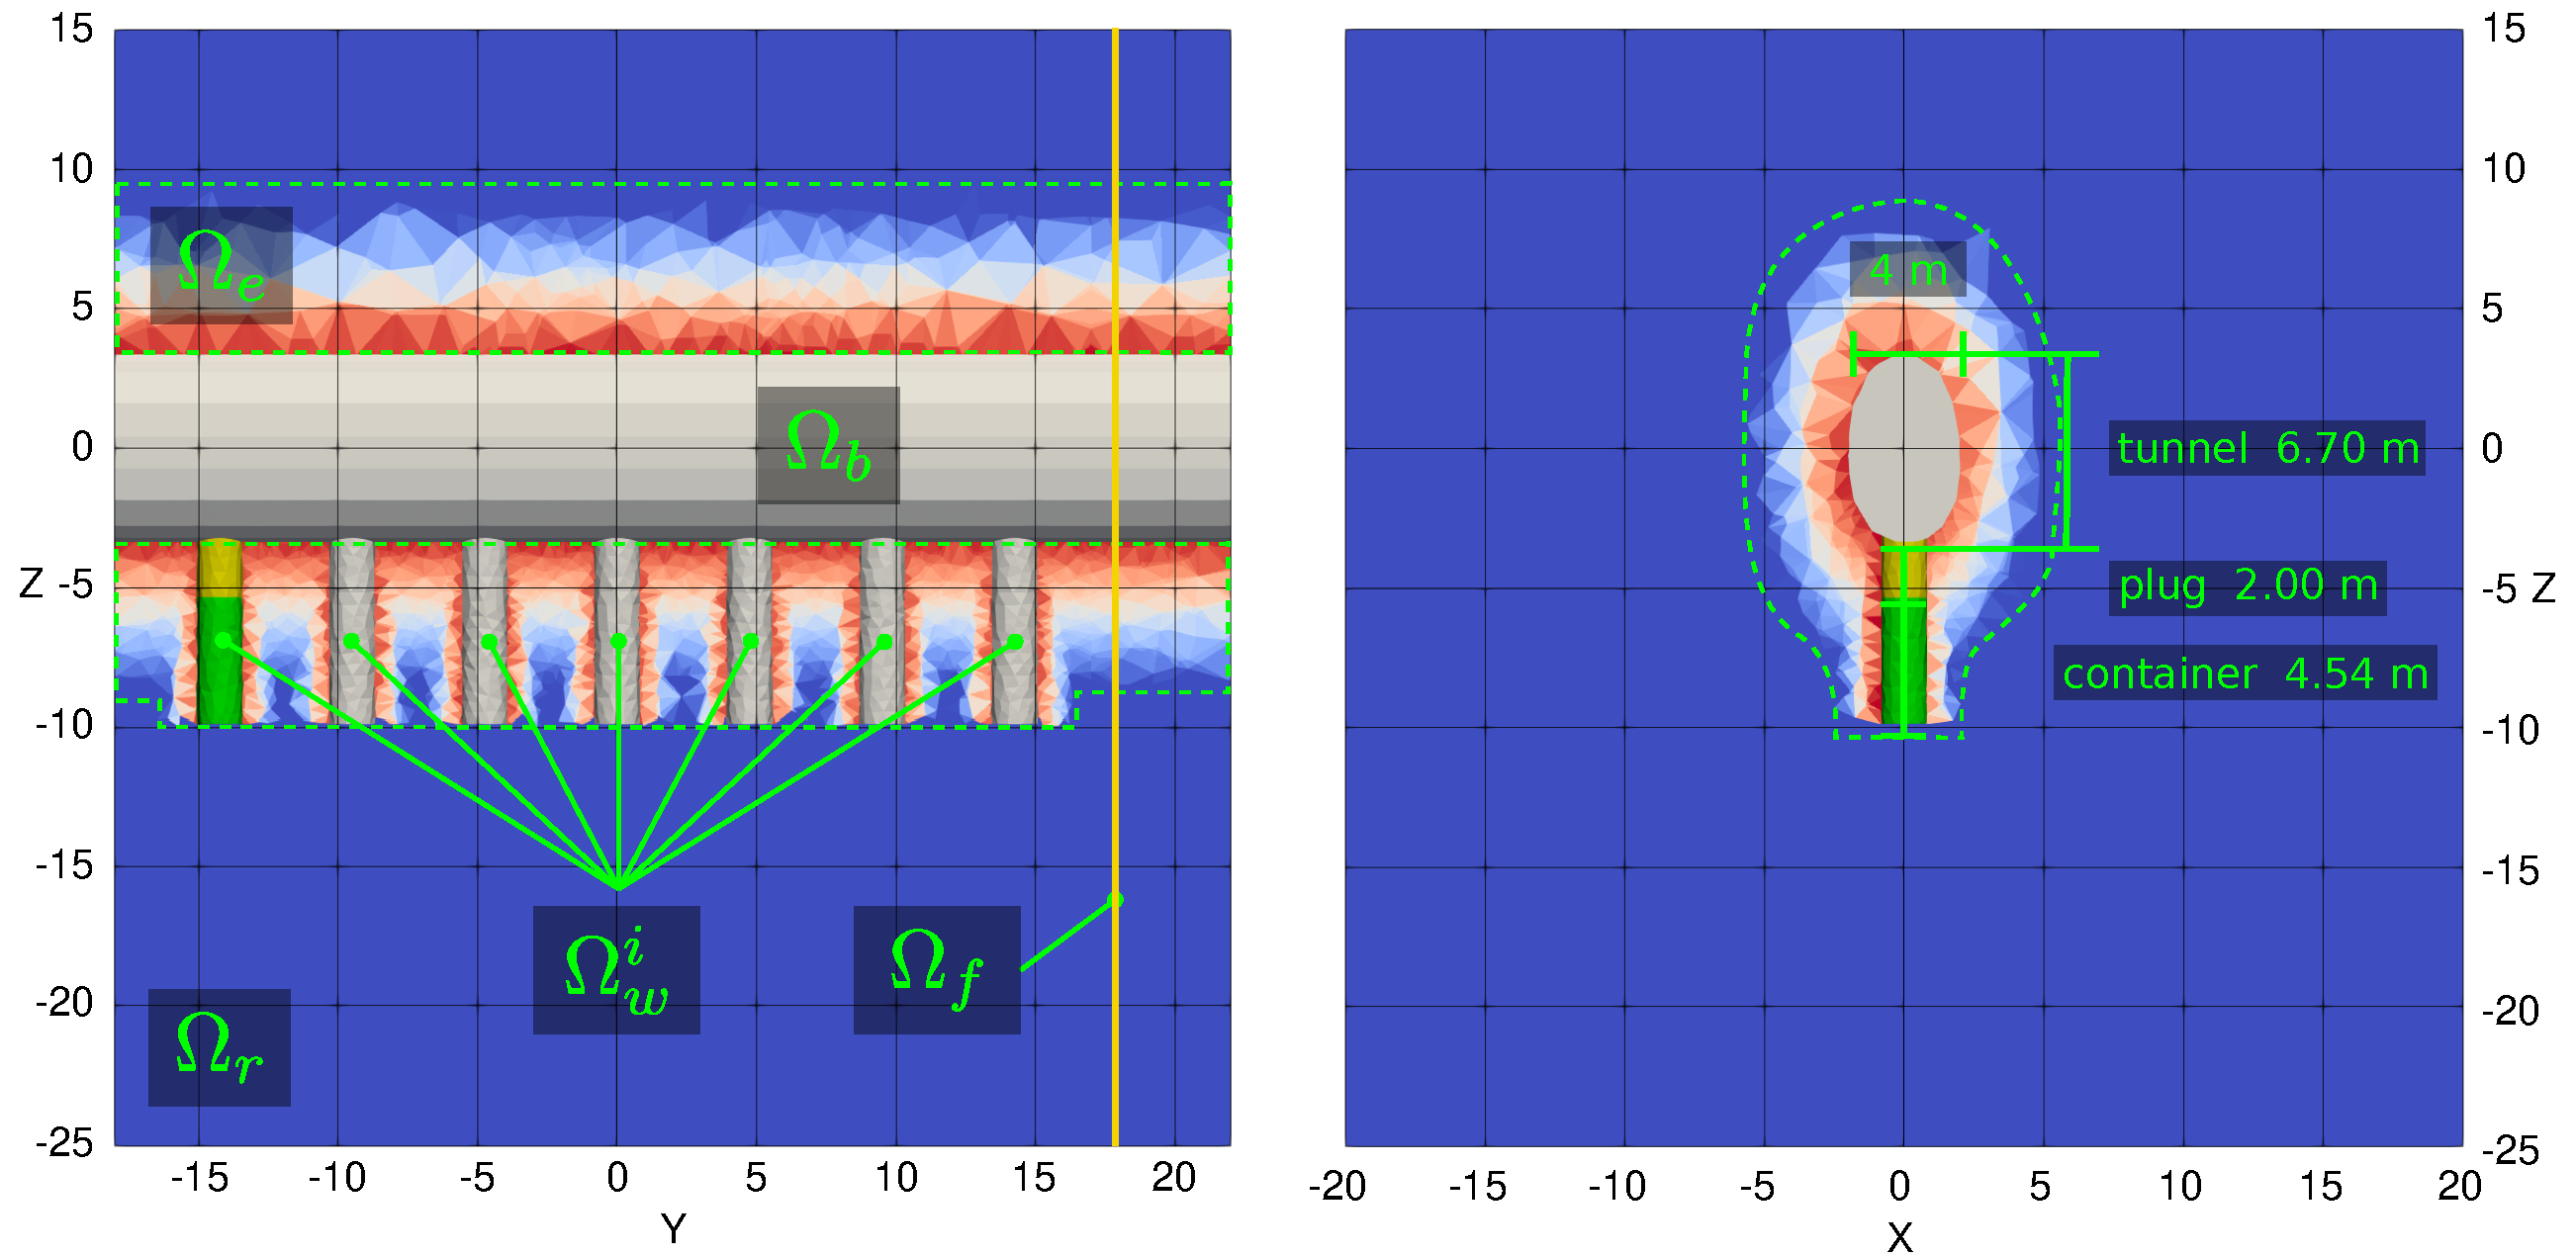
\includegraphics[width=\textwidth]{graphics_tr/cond_cut_edit.pdf}
\caption{Computational domains cuts in $xz$ and $yz$ planes domain with hydraulic conductivity field denoting the extent of the EDZ. Fractures are omitted.}
% TODO: smaller latex font
% \caption{TODO: Cut through the transport domain with fractures and permeability field denoting the extent of the EDZ}
\label{fig:conceptual}
\end{figure}

The disposal wells $\Omega_w^i$, $i=0,\dots, 6$, are represented by cylinders with dimensions following the \gls{WDP} design for VVER-440 waste.
Dimensions are, diameter $d_w=1.65\munit{m}$ and height $h_w=6.54\munit{m}$, including the $b_w=2\munit{m}$ spacer block. The actual waste package is not resolved, but the volumetric contamination source $f_w$ $\bunit{m^{-3}\cdot s^{-1}}$ is prescribed in the \gls{WDP} part below the spacer block. The source term is only applied to the most upstream well, $31\munit{m}$ from the fault zone. The volumetric source is proportional to the concentration difference over the whole volume of the source well:

\begin{equation}
\label{eq:pulse_source}
    f_w = \alpha_w\big(c_w(t) - c(t, \vc x)\big)
    \qquad \text{on $\Omega_w^0$}.
\end{equation}
To simplify interpretation of the results, we assume a 
unit 50-year concentration pulse in the waste package:
\[
c_w(t) = \chi_{(0,50)}(t).
\]
% c_w(t) ... bude jednickovy pulz v prvnim kroce 0-30 y

The coefficient $\alpha_w$ reflects the diffusion through the bentonite buffer:
\[
 \alpha_w = \frac{D_b}{ w}\frac{S}{V},
\]
where $D_b$ $\bunit{m^2\cdot s^{-1}}$ is the diffusion coefficient of bentonite,
$w=0.368\munit{{m}}$ is the buffer thickness, $S\approx 12.36 \munit{m}^2$ is the waste package surface (with $r=\frac{d_w}{2} - w=0.914\munit{m}$, 
$h=3.79\munit{m}$) and $V=2.97\munit{m^3}$
% PE:
% S = 0,914×3,79×3,14256 + 2*3,14256*0.25*0,914 = 12,32 m2
% V=4,54×0,25×3,14256×0,914×0,914 = 2,97 m3
is the whole source domain volume.
The buffer thickness above \gls{WDP}, $0.4\munit{m}$, and below, $0.35\munit{m}$, is approximated by $w$ for simplicity.



 
 All the well domains  $\Omega_w^i$ have transport properties common with the access tunnel domain $\Omega_b$ corresponding to the transport properties of the bentonite. The access tunnel $\Omega_b$ has a simplified smooth profile resulting from averaging the laserscan data from tunnels at \URFB
and vertically scaled to the design dimensions: height $6.7\munit{m}$, width $4\munit{m}$. Excavation of the access tunnel leads to increased permeability in the excavation disturbed zone $\Omega_e$. Original idea to use posterior data from inversion of the pore pressures experiment could not be implemented due to complex rock structure. The complex excavation induced changes in the transport properties were simplified to the geometrical interpolation between the maximal EDZ permeability $k_e$ and the permeability $k_r$ of the intact rock on the domain $
\Omega_r$ over the thickness of the EDZ $w_e$. See the histogram of hydraulic conductivity over mesh elements in \figref{fig:cond_histogram}.

The \Gls{DFM} approach combining 
a~heterogeneous continuum and a~stochastic \Gls{DFN} is applied in both rock domains $\Omega_e$ and $\Omega_r$. A~single major fault zone, represented by a~vertical fracture crossing the whole domain, is placed at the downstream end of the computational domain (vertical orange line in \figref{fig:conceptual} left).
It effectively transports
contamination to the (bottom) boundary where the safety indicator is evaluated.






\begin{figure}[htb]
\centering
% 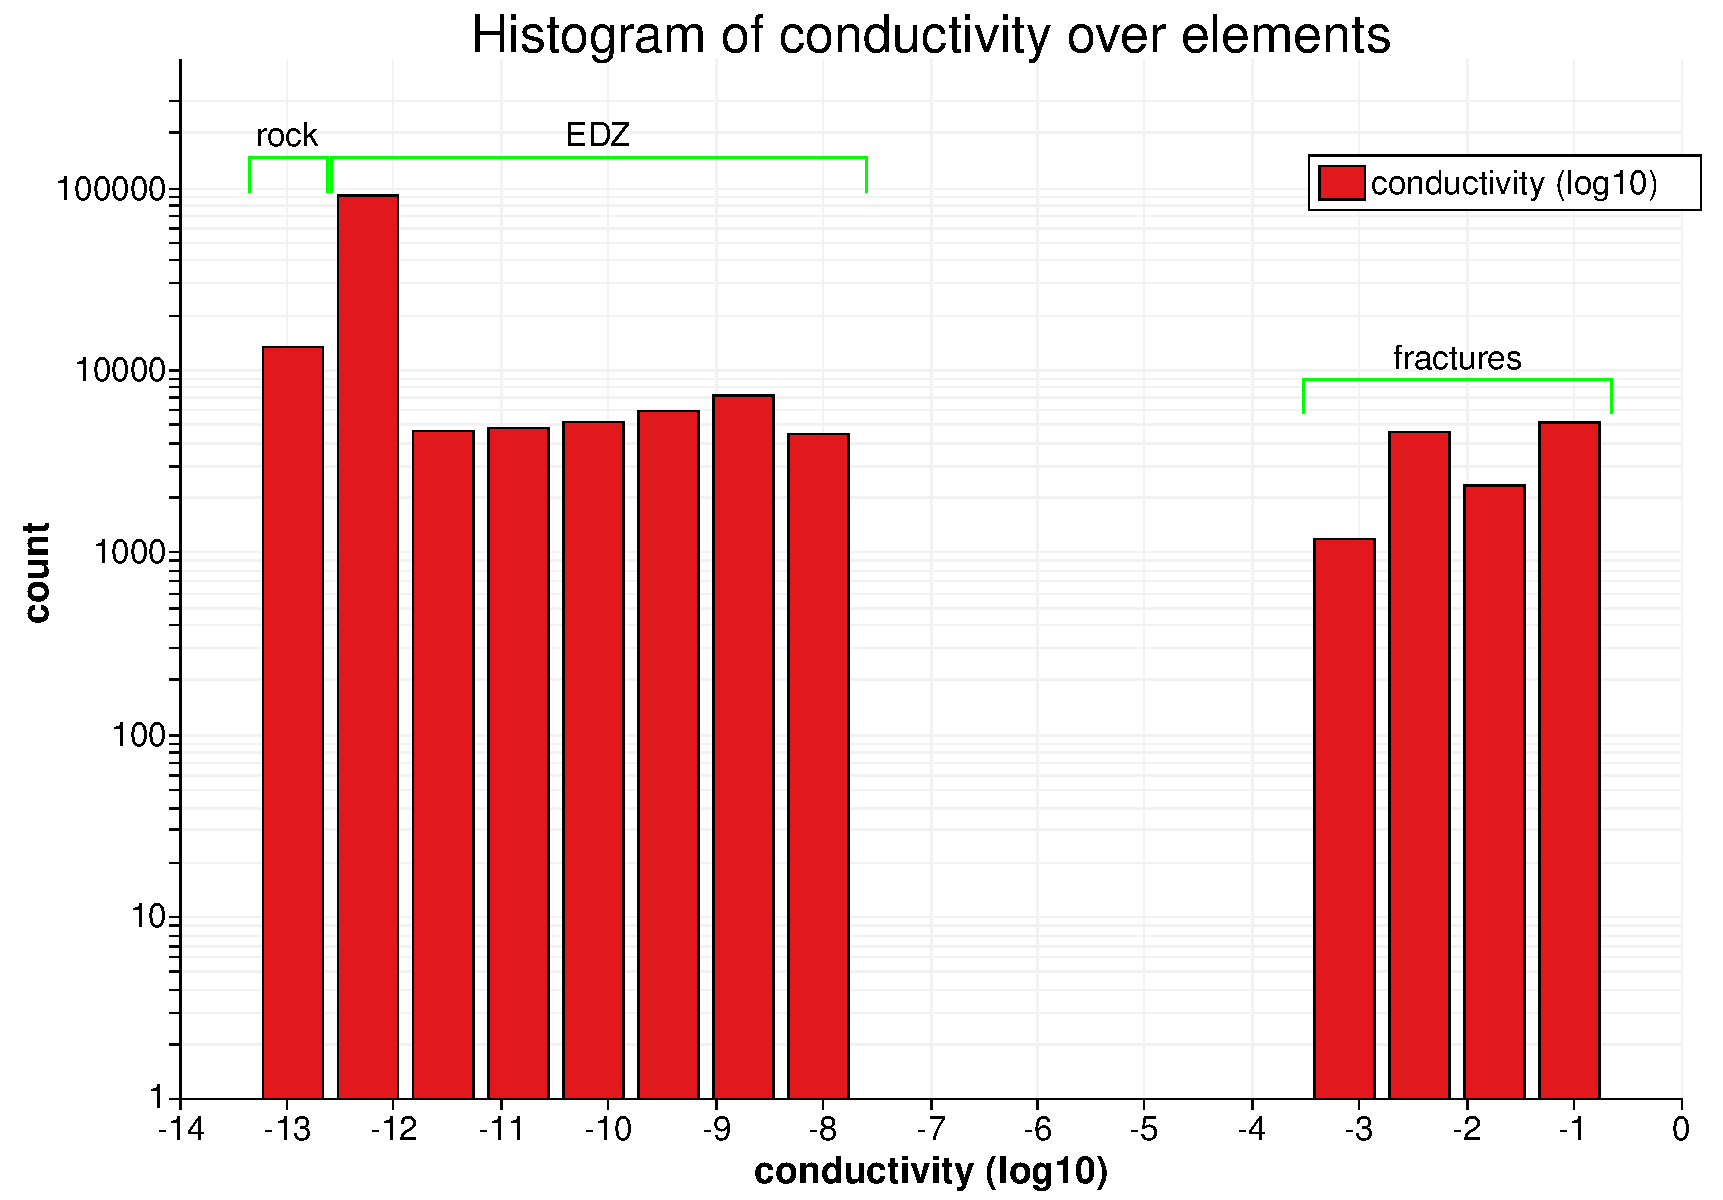
\includegraphics[width=0.75\textwidth]{graphics_tr/conductivity_hist_001_edit.pdf}
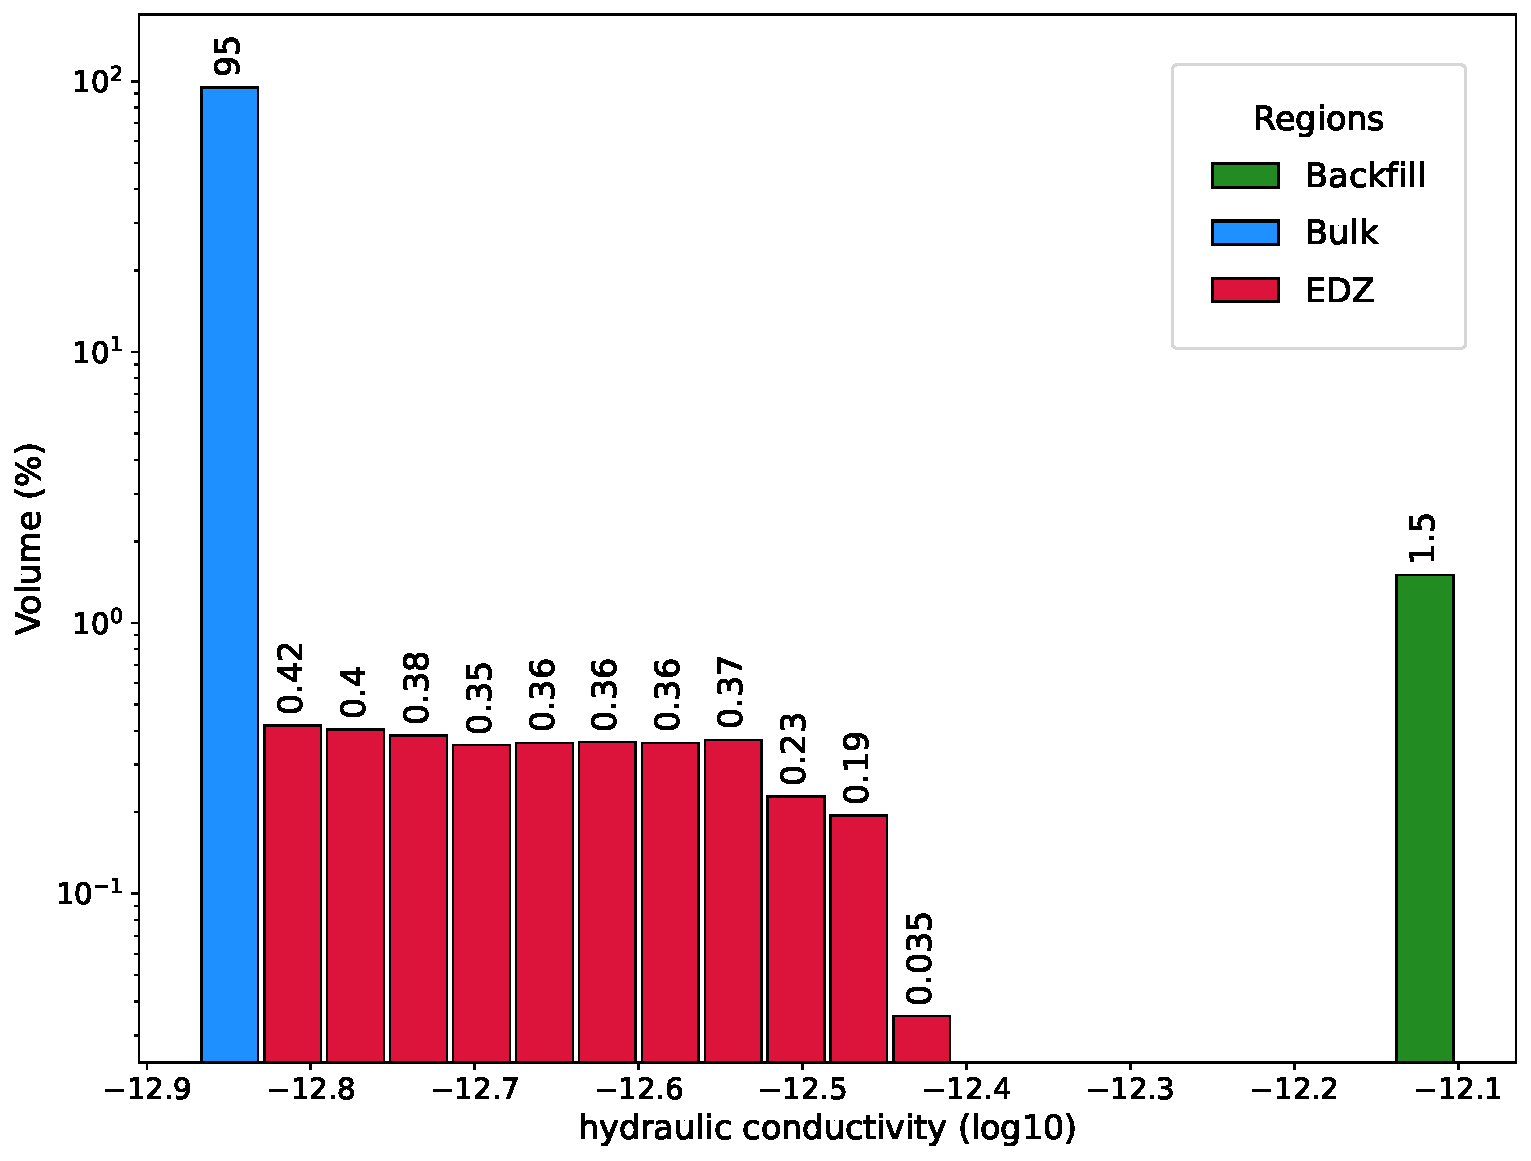
\includegraphics[width=0.75\textwidth]{graphics_tr/cond_hist.pdf}
\caption{Histogram of conductivity values (in $\log_{10}$ scale) over all computational mesh elements of a~randomly selected sample ($k_r=1.35\cdot10^{-13}\munit{m\cdot s^{-1}}$, $\tilde k_e=2.68$, $\tilde w_e=1.97$, $k_b=7.92\cdot10^{-13}$). We can clearly differentiate three domains: intact rock, EDZ and backfill.
}
\label{fig:cond_histogram}
\end{figure}


%%%%%%%%%%%%%%%%%%%%%%%%%%%%%%%%%%%%%%%%%%%%%%%%%%%%%%%%%%%%%%%%%%%%%%%%%%%%%%%%%%%%%%%
\subsection{Quantity of interest}
\label{sec:QoI}
Following the methodology by \cite{BrezinaMethodology2023}, we use a concentration-based safety indicator as the \Gls{QoI} for the sensitivity analysis. The decadic logarithm of the concentration field $c(t,\vc x)$ is evaluated on a grid of points $\vc X_i$, $i \in \mathcal I$, located on two horizontal planes near the top and bottom boundaries. The $99~\%$ percentile of these spatial values is used as a time-dependent QoI:
\[
    I(t) = Q_{0.99, i\in \mathcal I} \log_{10} c(t, \vc X_i).
\]
The aggregated (scalar) QoI is the $99~\%$ percentile over all space-time values:
\[
I  = Q_{0.99, i\in \mathcal I, j\in \mathcal J} \log_{10} c(t_j, \vc X_i),
\]
where $\mathcal J$ denotes the index set of discrete time steps $t_j$.

Example of a~DFN including a concentration cloud can be seen in \figref{fig:conc_cloud_fractures}.
In the same figure, two parallel planes near the top and bottom of the model domain are apparent. The computed concentration is interpolated onto these planes (2D structured grids of size $20\times20$), and the resulting values are used to determine 
the quantity of interest.

\begin{figure}[htb]
\centering
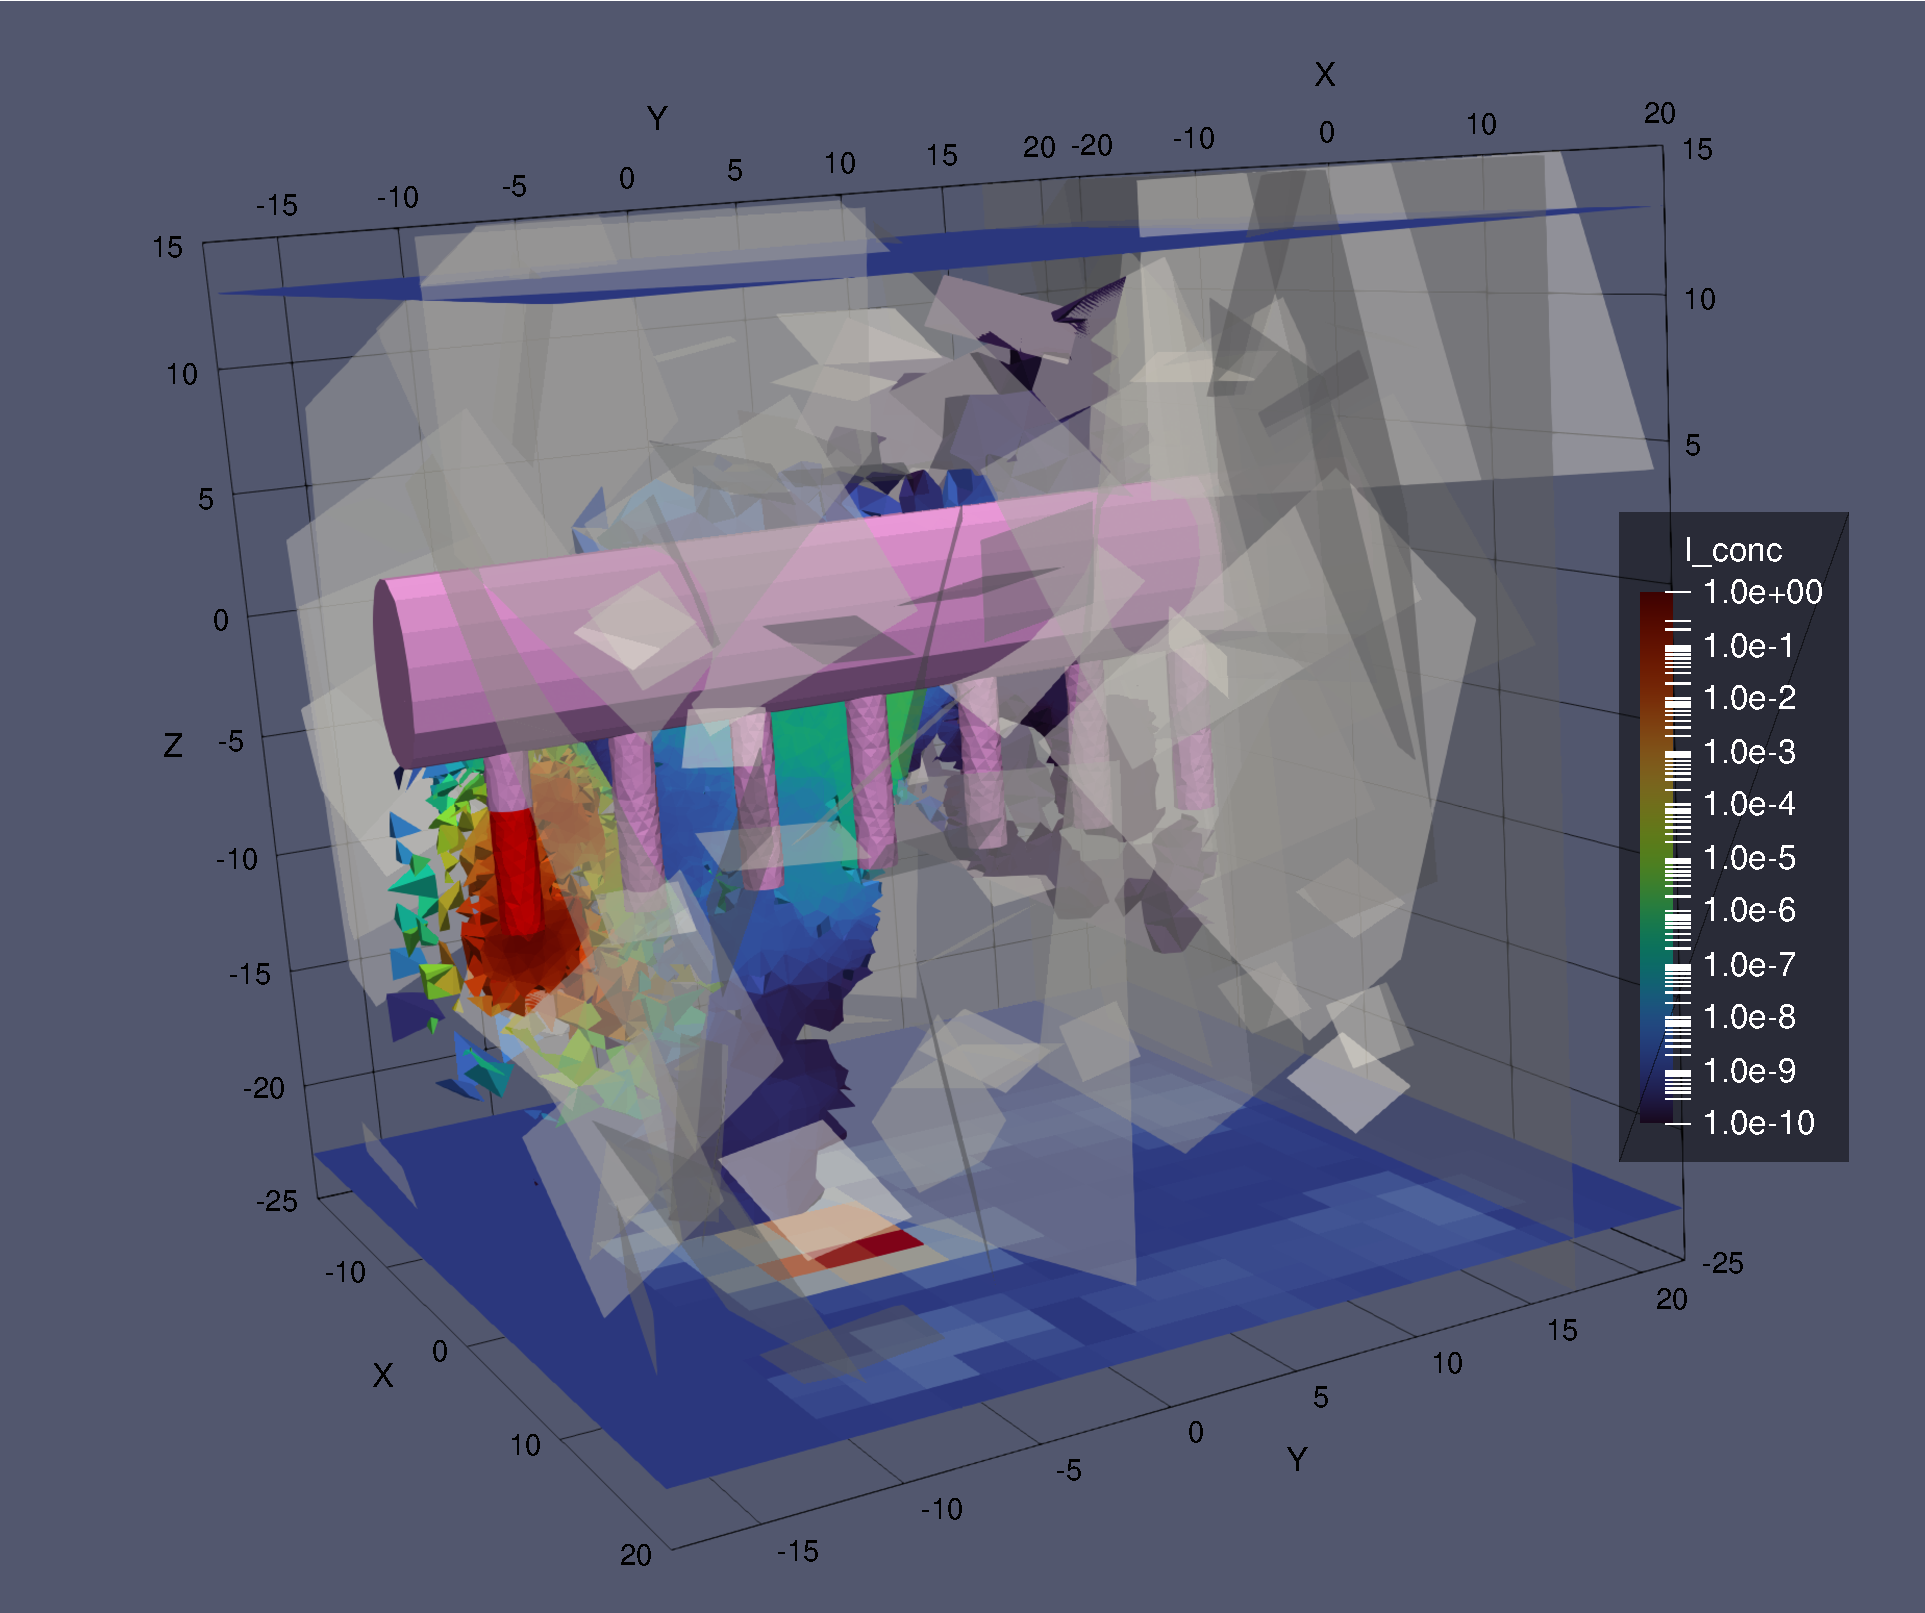
\includegraphics[width=0.75\textwidth]{graphics_tr/conc_cloud_001.pdf}
\caption{Example of the stochastic \gls{DFN} (transparent gray planes) in the computational domain at simulation time $500\,\munit{y}$. The concentration cloud is displayed in logarithmic color scale, together with the evaluation planes near the top and bottom boundaries.}
\label{fig:conc_cloud_fractures}
\end{figure}

\subsection{Advection-diffusion equations}
Contaminant transport is caused by groundwater flow, which is described by the continuity equation and Darcy's law for low velocities. For long-term steady-state conditions, the stationary form of the flow equations can be considered as:
\begin{equation}
    \label{eq:darcy_matrix}
    \div \vc v = 0, \quad \vc v = -\tn K \grad (p + z),
\end{equation}
where $\vc v$ $\bunit{m\cdot s^{-1}}$ is the Darcy (macroscopic) flow velocity, $\tn K$ $\bunit{m\cdot s^{-1}}$ is the hydraulic conductivity tensor, $p$ $\bunit{m}$ is the pressure head, and $z$ $\bunit{m}$ is the vertical component of the position vector. When modeling transport through the EDZ, the hydraulic conductivity tensor, which can be significantly heterogeneous and anisotropic, plays an important role.
% The influence of the EDZ on $\tn K$ will be described in Chapter \ref{sec:poroelasticity} using the poroelastic model.

After solving the equation \eqref{eq:darcy_matrix} with suitable boundary conditions and obtaining the velocity field $\vc v$, the time evolution of the concentration of the conservative tracer $c$ $\bunit{kg\cdot m^{-3}}$ can be described by the advection-diffusion equation:
\begin{equation}
   \label{eq:transport_matrix}
   \prtl_t (\theta c) + \div(\vc j) = f_w,\quad \vc j = \vc v c - \theta \tn D \grad c,
\end{equation}
where $\theta$ $\bunit{-}$ is the porosity, $\tn D$ $\bunit{m^2\cdot s^{-1}}$ is the diffusion and hydrodynamic dispersion tensor, hereafter referred to as the {\it dispersion tensor}. Diffusion is due to the chaotic motion of solution molecules, while dispersion is due to velocity field inhomogeneity at the microscopic level.
% , see  Section \ref{sec:transport_multiscale}.
For the case of an isotropic medium, the dispersion tensor is given:
\begin{equation}
  \label{eq:dispersion_tn}
  \tn D = \tn D_e + \abs{\vc u}\Big(\alpha_T \tn I + (\alpha_L - \alpha_T)\frac{\vc u \otimes \vc u}{\abs{\vc u}^2}\Big),
\end{equation}
where
\begin{itemize}
 \item $\tn D_e = d_e \tn I$ is the molecular diffusion tensor, which for simplicity, we consider to be isotropic with a~coefficient of effective diffusion $d_e$ $\bunit{m^2\cdot s^{-1}}$, on the order of $10^{-9}$ for pure water,
%$[-]$ is the tortuosity according to \cite{millington_permeability_1961},
 \item $\alpha_L$ and $\alpha_T$ $\bunit{m}$ are the longitudinal and transverse dispersion coefficients,
 \item $\vc u$ is the pore velocity, $\vc u = \vc v / \theta$.
\end{itemize}

The contaminant volumetric source $f_w$ (right hand side in \eqref{eq:transport_matrix}) is constrained in time and space to the single pulse in the leaking  \gls{WDP} described by  \eqref{eq:pulse_source}.

Radioactivity decay and sorption strongly influence the evolution of the specific radionuclides' concentration. To simplify the calculations and especially the interpretation of the results, the influence of these phenomena is not considered in this study.
% The Flow123d simulator implements both phenomena in full generality. We show below that the simplification is acceptable for relative comparisons of WDP positions in the case of homogeneous $\theta$ porosity and sorption.


%%%%%%%%%%%%%%%%%%%%%%%%%%%%%%%%%%%%%%%%%%%%%%%%%%%%%%%%%%%%%%%%%%%%%%%%%%%%%%%%%%%%%%%
\subsection{Vector calculus for DFM}
\label{sec:vek_pocet_dfm}
The DFM setting combines processes in the rock matrix with processes on a lower-dimensional fracture network. The resulting model is inherently *mixed-dimensional*: the governing equations live on manifolds of different dimension and are coupled through interface terms. Most ambiguities arise in the coupling terms (traces, normal fluxes, and sign conventions). We therefore fix a systematic mixed-dimensional vector calculus, following \cite{BrezinaMethodology2023} and consistent with \cite{flow123d}. The purpose is clarity and reproducibility: once the operators and interface mappings are set, the weak formulation and discretization follow without ad-hoc conventions.

We denote $\Omega_m \subset \Real^3$ as the matrix region and $\Omega_f=\Cup_{i=1}^{n_{fr}}\mathcal F_i$ as the fracture region, assuming that the individual fractures $\mathcal F_i$ have a~polygonal shape.
%$\mathcal F_i: D_i to \Real^3$ are parametrically defined polygons.
% \sy{[Standa: For the purposes of this report, I think it is not necessary to state that fractures are parametrically defined. Also, consider introducing the notation $\Omega=\Omega_m\cup\Omega_f$, where the symbol $\Omega$ would be used for the definition of continuous models, e.g., in section 2.1, which is currently missing.]}
% \jb{It is good to realize that quantities on fractures are functions of only two parametric coordinates.}
For simplicity, we will not discuss fracture intersections further; however, the implementation used in the Flow123d simulator accounts for them. For a~given scalar, vector, or tensor quantity $p=(p_m, p_f)$, we denote $p_m$ as the function of the quantity in $\Omega_m$ and $p_f$ as the function defining the quantity in $\Omega_f$ (in fact, the function is defined on the parametric domains $D_i$). For each point $\vc x \in \Omega_f$ on an individual fracture, we denote $\vnu(\vc x)$ as the normal vector, also defining its orientation. We further distinguish the positive and negative sides of the plane $\vnu^+ = \vnu$ and $\vnu^-=-\vnu$. The quantity $p$ can be discontinuous in the normal direction to the fracture, hence for $p_m$, we define its value on the sides of the fracture: $p_m^+$, $p_m^-$. The fracture thickness field is denoted as $\delta(\vc x)$.

To simplify the notation of equations on fractures, we now introduce semi-discrete differential operators. For a~scalar quantity $p$, $p_f$ is a~function of two variables, and its tangential gradient $\grad_t p_f$ is a~tangential vector to $\Omega_f$. The semi-discrete gradient then approximates the normal component using the difference of traces:
$$
\fgrad p = \grad_t p_f + \grad_\nu p,\qquad 
\grad_\nu p = \frac{1}{2}\Big(\Delta^+ p\vnu^+  + \Delta^- p\vnu^-\Big),
$$
where the normal component is approximated by the sum of differences across the sides of the fracture:
$$
\qquad \Delta^\pm p = \frac{2}{\delta}\Big(p_m^\pm - p_f\Big).
$$
We further define the semi-discrete gradient on the positive and negative sides of the fracture plane:
$$ \fgrad^\pm p = \grad_t p_f + \Delta^\pm p\vnu^\pm. $$
This definition allows the formal extension of notation for fracture intersections.
% \todo{It appears that equations can indeed be written with these summed operators, but for the writing of the Neumann boundary condition, which forms the link, we still need to introduce $\fgrad^\pm$.}

In the same manner, we introduce the gradient for a~vector field $\vc v=(\vc v_m, \vc v_f)$:
$$
\fgrad \vc v = \grad_t \vc v_f + \grad_\nu \vc v,\qquad 
\grad_\nu \vc v = \frac{1}{2}\Big(\Delta^+\vc v \otimes\vnu^+  + \Delta^- \vc v\otimes\vnu^-\Big),
$$
Similarly, we then introduce the semi-discrete divergence of a~vector field:
$$
\fdiv \vc v = \div_t \vc v_f + \div_\nu \vc v,\qquad
\div_\nu \vc v = \frac{1}{2}\Big(\Delta^+ \vc v \cdot \vnu^+  + \Delta^- \vc v \cdot \vnu^-\Big)
$$
Here, the tangential divergence $\div_t \vc v_f$ is the divergence of the tangential component of the field $\vc v_f$. Similarly, we introduce the divergence for a~tensor quantity $\vc\sigma = (\vc\sigma_m, \vc\sigma_f)$:
$$
\fdiv \vc\sigma = \div_t \vc\sigma_f + \div_\nu \vc\sigma,\qquad
\div_\nu \vc\sigma = \frac{1}{2}\Big(\Delta^+ \vc\sigma \vnu^+  + \Delta^- \vc\sigma \vnu^-\Big).
$$


%%%%%%%%%%%%%%%%%%%%%%%%%%%%%%%%%%%%%%%%%%%%%%%%%%%%%%%%%%%%%%%%%%%%%%%%%%%%%%%%%%%%%%%
\subsection{Transport equations for DFM description}
\label{sec:transport_DFN}

For the DFM description, equation \eqref{eq:darcy_matrix} is considered only in the matrix region $\Omega_m$. In the fracture network $\Omega_f$, the flow is described by the equation:
\begin{equation}
    \label{eq:darcy_fracture}
    \fdiv (\delta \vc v_f) = 0, \quad \vc v_f = -\tn K_f \fgrad (p + z).
\end{equation}
Here, $\tn K_f(\vc x)$ is the 3D conductivity tensor describing the material of the fracture network. The coupling between the regions is given by the balance of volumetric flux at the interfaces between the matrix and the fracture, which represents a~Neumann boundary condition for equation \eqref{eq:darcy_matrix} on $\Omega_m$. A~separate condition must be considered for each side of the fracture:
\begin{equation}
    \vnu^{\pm} \cdot \vc v_m^\pm = \vnu^{\pm} \cdot \vc v_f^\pm =  
    -\vnu^\pm \cdot \left(\tn K_f \fgrad^\pm (p + z)\right)
    \quad \text{on }\Omega_f.
\end{equation}
For the flow model, we consider a~Dirichlet boundary condition for the piezometric head $P = p + z$, which is interpolated from the regional flow model at the model location.

Similarly, for the DFM description of transport, we consider 
equation \eqref{eq:transport_matrix} only for the matrix $\Omega_m$,
while in the fractures $\Omega_f$, the transport equation takes the form:

\begin{equation}
   \label{eq:transport_fr}    
   \prtl_t (\delta\theta c_f) + \fdiv \,\vc j = 0, \quad  
   \vc j_f = \vc v_f c_f - \delta \theta \tn D \fgrad c.
\end{equation}
The coupling between the regions, similar to flow, is given by the balance of the tracer mass flux:
\begin{equation}
    \vnu^{\pm} \cdot \vc j_m^\pm  = \vnu^{\pm} \cdot \vc j_f^\pm  \quad \text{on }\Omega_f.
\end{equation}
At the outer boundary of the model, a~zero mass flux is considered at the inflow part of the boundary, and a~zero diffusive flux is considered at the outflow part of the boundary.

\def\rmin{\underline r}
\def\rmax{\overline r}
\subsection{Stochastic model of fracture network}
As Darcy flow in crystalline rock is primarily attributed to fractures, discrete fracture network (DFN) models are commonly employed by \cite{deDreuzy2012Influence}. Our DFM approach 
applies the same stochastic model of the fractures, where, however, just a small range of the largest fractures is discretized explicitly, while smaller-scale fractures are represented by upscaled heterogeneous material fields. In particular, we adopt the DFN parametrization 
from SKB report by \cite{Ohman_Site_2010}.
\begin{enumerate}
\item Based on evidence from nature, \cite{Bonnet_Scaling_2001}, we assume a truncated power-law distribution of the fracture sizes:
\begin{equation}
    \label{pow_law}
    f_s \sim C r^{-\alpha},
    \qquad
    C = \frac{1-\alpha}{\rmax^{1-\alpha} - \rmin^{1-\alpha}},
\end{equation}
where $\alpha$ represents the characteristic exponent, while $\rmin$ and $\rmax$ denote the minimum and maximum lengths of a fracture, respectively. The $\rmin$, $\rmax$ are rather arbitrary parameters providing a scale window where the power-law is assumed. 

\item Poisson process is assumed for the centers of the fractures. The density parameter
$P_{32}$  $[m^{-1}]$ is the average total surface area of the fracture of size $r\in(\rmin, \rmax)$ within a unit volume. Alternatively, dimensionless and scale-independent density could be used to better describe the connectivity of DFN, see \cite{Adler1999} for details.

\item  
The distribution of orientations is modeled by Fisher distribution. Five families of fractures with significantly different orientations are considered.


\item We adopt the power-law model for fracture transmissivity from \cite{Ohman_Site_2010} in a dimensionless form,
\[
    T = \delta K_f = a\left(\frac{r}{r_0}\right)^{b},
\qquad r_0 = 1\,\mathrm{m},
\]
where $T$ is the fracture transmissivity $[\,\mathrm{m^2\,s^{-1}}\,]$, $\delta$ is the hydraulic aperture
$[\,\mathrm{m}\,]$, $K_f$ is the fracture hydraulic conductivity $[\,\mathrm{m\,s^{-1}}\,]$,
and $r$ is the fracture radius $[\,\mathrm{m}\,]$.

Using the cubic law with a constriction factor $f_K$ $[-]$,
\begin{equation}
    \label{eq:k_frac}
    K_f = f_K \frac{g \rho_w}{12\mu}\,\delta^{2},
\end{equation}
where $g$ is the gravitational acceleration $[\,\mathrm{m\,s^{-2}}\,]$,
$\rho_w$ is the water density $[\,\mathrm{kg\,m^{-3}}\,]$, and
$\mu$ is the dynamic viscosity of water $[\,\mathrm{Pa\,s}]$.
Substituting \eqref{eq:k_frac} into $T=\delta K_f$ yields
aperture:
\begin{equation}
    \label{eq:k_frac_1}
    \delta = \alpha \left(\frac{r}{r_0}\right)^{\beta},
    \qquad
    \alpha = \left(\frac{12\mu\,a}{f_K g \rho_w}\right)^{\!1/3},
    \qquad
    \beta = \frac{b}{3}.
\end{equation}
Here $\beta$ is dimensionless and $\alpha$ has units $[\,\mathrm{m}\,]$, as expected for an aperture.


\end{enumerate}

For simplicity, we assume uncorrelated fractures with positions determined by a Poisson process and independent orientations. See 
\cite{Sahimi20110420, Liu2016} for more general models.
% Additionally, we consider the cubic law for fracture hydraulic conductivity:



% \paragraph{(To be moved) Péclet number including mechanical dispersion.}
% In steady saturated conditions, the solute flux is written as
% \[
% \mathbf{J}=\mathbf{q}\,C \;-\; n D_e \nabla C \;-\; n \mathbf{D}_{\mathrm{disp}}\nabla C,
% \qquad \mathbf{q}=-k\nabla h,
% \]
% with a longitudinal dispersion closure
% \[
% \mathbf{D}_{\mathrm{disp}} \approx \alpha_L|\mathbf{q}|\,\mathbf{e}_q\mathbf{e}_q^{\mathsf T}
% \quad (\alpha_T \ll \alpha_L).
% \]
% For one-dimensional transport along the mean flow direction, the total macroscopic spreading
% coefficient is
% \[
% D_{\mathrm{tot}} \equiv D_e + \alpha_L |\mathbf{q}|.
% \]
% A convenient advection--spreading indicator is then
% \[
% \mathrm{Pe}_{\mathrm{tot}}=\frac{|\mathbf{q}|\,L_C}{n\,D_{\mathrm{tot}}}
% =\frac{|\mathbf{q}|\,L_C}{n\,(D_e+\alpha_L|\mathbf{q}|)}.
% \]
% Here $L_C$ is the characteristic length of the concentration gradient in the problem at hand
% (e.g.\ thickness of a concentration boundary layer, width of a source zone, or a representative
% transport length over which the gradient is established), and should be chosen consistently with the
% model setup rather than automatically set equal to the full domain size.

\subsection{Boundary conditions}
The steady Darcy flow is driven by a Dirichlet boundary condition imposed on the outer boundary of the bulk domain. We prescribe a homogeneous gradient of the piezometric head,
\[
p(x,y,z) = 0.05\,(-y + 0.1z),
\]
which induces a gently decreasing mean velocity field parallel to the tunnel
(in $y$  direction). The resulting velocity magnitude is on the order of $10^{-11}$, comparable to the groundwater velocity at the repository domain in the hydrological model of the test locality \textquote{Kraví hora}. To avoid unrealistically high fluxes along fractures (in particular the large collecting fracture), we exclude fractures from the boundary condition enforcement.

The advection--diffusion equation is driven by an inflow boundary condition: the diffusive flux is set to zero on the entire boundary, and the concentration is set to zero on the inflow portion. Because the problem is diffusion-dominated, the zero diffusive-flux condition can be viewed as a conservative approximation, as it prevents outward diffusive loss and thus tends to increase the resulting concentration of the safety indicator.


\subsection{Heterogeneous fields}
\label{sec:parameters}

The model includes matrix parameters defined as spatially variable fields. Rock and bentonite are represented as separate domains. Bentonite is treated as relatively homogeneous, whereas the rock mass is heterogeneous due to (i) excavation-induced effects caused by stress redistribution and (ii) sub-element-scale fractures that introduce random variability. We address the former via \gls{EDZ} parametrization; the latter requires a non-Gaussian stochastic representation and is the subject of ongoing research.

\def\edzRelThick{{\color{red}\tilde{w}_e}}
\def\edzPerm{{\color{red}\tilde{k}_e}}
\def\iPerm{{\color{blue}k_r}}
\def\edzPor{{\color{red}\tilde{\theta}_e}}
\def\iPor{{\color{blue}\theta_r}}

\paragraph{EDZ fields}
In Section \ref{sec:hm_steady}, we study the expected permeability changes induced by excavation. However, because the homogeneous model used there does not match the experimental data described in Chapter \ref{ch:inversion}, we neglect the potentially significant angular variability associated with the orientation of the maximum initial stress. Instead, we adopt a simplified model that considers only radial variability, and we use the permeability range predicted by the HM model to prescribe uncertainty (discussed later in Section \ref{sec:parameters}).

The scalar permeability $k(\vc x)$ is interpolated on a logarithmic scale (i.e., using geometric progression) between the most perturbed permeability $k_e=\edzPerm\,\iPerm$ at the tunnel wall and the intact rock permeability $\iPerm$ at the outer boundary of the EDZ:
\begin{equation}
    \label{eq:edz_perm}
    \log k(\vc x) = (1-t)\,\log(k_e) + t\,\log(\iPerm),
    \qquad
    t=\frac{d(\vc x)-1}{\edzRelThick-1}.
\end{equation}
Here $d(\vc x)$ denotes the distance from the tunnel axis, normalized by the tunnel radius, so that $d=1$ at the tunnel wall. The parameter $\edzRelThick$ defines the outer boundary of the EDZ as a multiple of the tunnel radius.

Similarly, we prescribe the spatially variable porosity as
\begin{equation}
    \label{eq:edz_por}
    \theta(\vc x) = (1-t)\,\theta_e + t\,\theta_r,
    \qquad
    \theta_e = \edzPor\,\iPor.
\end{equation}

The red parameters $\edzRelThick$, $\edzPerm$, and $\edzPor$ characterize the EDZ, while the blue parameters correspond to intact rock.

\paragraph{Dispersion}
Dispersion is an apparent spreading caused by spatial variability in the velocity field, which in turn reflects heterogeneity in permeability. Although we do not explicitly model random spatial heterogeneity in the conductivity (permeability) field, its macroscopic effect can be represented through an effective dispersion.

Using first-order stochastic theory for macroscopic dispersion \cite{Zech_Evidence_2023}, the longitudinal dispersivity is proportional to the variance of $\ln K$ and to the integral scale $I_h$:
\begin{equation}
    \alpha_L = \sigma_{\ln K}^2\, I_h .
\end{equation}
In our case, we take $\sigma_{\ln K}^2$ to be the same variance used to represent uncertainty in the bulk permeability. The integral scale is bounded above by the characteristic size of the largest unresolved fractures (approximately $5\,\mathrm{m}$) and below by the mesh size (approximately $0.5\,\mathrm{m}$). Following a common rule of thumb, we set the transverse dispersivity to one tenth of the longitudinal value.

%\paragraph{Dispersivity.}












% \pe{
% \subsection{Numerical scheme and HPC computation}

% Numerical solutions of transport problems are carried out using the Flow123d software. In particular, the flow equations \eqref{eq:darcy_matrix} and \eqref{eq:darcy_fracture} are solved by a mixed-hybrid method employing zero-order Raviart–Thomas elements for the discretization of the velocity field and piecewise-constant elements for the discretization of pressure head. Flux continuity is enforced by Lagrange multipliers on element faces. The computational domain is partitioned into simplicial elements such that the 2D fracture elements coincide with the faces of the adjacent 3D elements. The discretized problem then admits the algebraic representation

% \begin{equation}
% \label{eq:flow_alg_mh} 
% \begin{bmatrix}
% \tn F^{\vc v\vc v} & \tn B^{\vc v p} & \tn B^{\vc v\lambda}\\
% (\tn B^{\vc v p})^\top & \tn O & \tn O\\
% (\tn B^{\vc v\lambda})^\top & \tn O & \tn O
% \end{bmatrix}
% %
% \begin{bmatrix}
% \uu^{\vc v}\\ 
% \uu^p\\
% \uu^\lambda
% \end{bmatrix} = 
% %
% \begin{bmatrix}
% \vc 0\\
% \vc f^p\\
% \vc 0
% \end{bmatrix}, 
% \end{equation}

% where $\uu^{\vc v}$, $\uu^p$, and $\uu^\lambda$ denote the degrees of freedom associated with the velocity field, the pressure head at element centroids of the computational mesh, and the Lagrange multipliers, respectively. The vector $\vc f^p$ represents the discretized source term in the mass balance. The matrices $\tn F^{\vc v\vc v}$ and $\tn B^{\vc vp}$ are assembled locally on an element-by-element basis, which enables an efficient evaluation of the Schur complement. Consequently, the linear system \eqref{eq:flow_alg_mh} can be reduced to a system for $\uu^\lambda$ with a symmetric positive definite matrix, which is solved using the preconditioned conjugate gradient method.

% The transport equations \eqref{eq:transport_matrix} and \eqref{eq:transport_fr} are solved using the discontinuous Galerkin method (DGM). We typically employ first- or second-order elements. For improved robustness with respect to the advection-to-diffusion (dispersion) ratio, a non-symmetric variant of DGM is adopted, leading to the algebraic system

% $$ \tn T\uu^c = \vc f^c $$
% with a generally non-symmetric matrix. The system is solved by the $BiCGStab$ method with suitable preconditioning.

% }
\subsection{Numerical scheme and HPC computation}

The numerical simulations of flow and transport are performed with the \emph{Flow123d} software. The Darcy flow equations \eqref{eq:darcy_matrix} and \eqref{eq:darcy_fracture} are discretized by a mixed--hybrid finite element method: the velocity field is approximated using lowest-order Raviart--Thomas (RT0) elements, while the pressure head is represented by piecewise-constant  elements. Flux continuity across element interfaces is enforced by Lagrange multipliers defined on element faces. The computational mesh consists of simplices, and it is constructed so that 2D fracture elements coincide with faces of the adjacent 3D bulk elements. The resulting discrete problem can be written in the block form:
\begin{equation}
\label{eq:flow_alg_mh} 
\begin{bmatrix}
\tn A_{\vc v\vc v} & \tn B_{\vc v p} & \tn B_{\vc v\lambda}\\
\tn B_{\vc v p}^\top & \tn O & \tn O\\
\tn B_{\vc v\lambda}^\top & \tn O & \tn O
\end{bmatrix}
%
\begin{bmatrix}
\uu^{\vc v}\\ 
\uu^p\\
\uu^\lambda
\end{bmatrix} = 
%
\begin{bmatrix}
\vc 0\\
\vc f^p\\
\vc 0
\end{bmatrix}, 
\end{equation}
where $\uu^{\vc v}$, $\uu^p$, and $\uu^\lambda$ denote the degrees of freedom associated with the velocity field, the pressure head at mesh element centroids, and the Lagrange multipliers, respectively. The vector $\vc f^p$ represents the discrete source term in the mass balance. The matrices $\tn A_{\vc v\vc v}$ and $\tn B_{\vc v p}$ are assembled only locally on an element-by-element basis, which allows for an efficient per-element construction of the Schur complement. Consequently, the saddle-point system \eqref{eq:flow_alg_mh} can be reduced to a system for $\uu^\lambda$ with a symmetric positive definite matrix, which is solved using a CG method with an algebraic multigrid preconditioning.

The transport equations \eqref{eq:transport_matrix} and \eqref{eq:transport_fr} are discretized using the discontinuous Galerkin method (DGM), typically with first- or second-order polynomial approximation. To improve robustness across a wide range of advection-to-diffusion ratios, we employ a non-symmetric DGM variant, which leads to a nonsymmetric algebraic system. solved using the GMRES method with ILU preconditioning.


\section{Influence of bentonite backfill on the hydraulic and mechanical properties of the near field}
\label{sec:hm_steady}
A hydro-mechanical simulation was performed to assess the impact of excavation and  bentonite backfilling on the permeability and mechanical stress in the surrounding rock.
We analyzed the influence of the relaxation time, the magnitude of the swelling pressure, and the orientation of the access tunnel.

The computational domain corresponds to the geometry of the conceptual model (depicted in Fig. \ref{fig:conceptual}); however, in contrast to the transport model, the tunnel and the disposal wells were excluded.
A poro-elastic model was used with rock parameters identical to those used in the HM model in Chapter \ref{ch:model_comparison}.
In particular, the hydraulic conductivity was assumed to be dependent on the mechanical stress via the relation \eqref{eq:conductivity_relation}.


The simulation period was 200 years to capture the following key time points (see also Fig.~\ref{fig:hm_bentonit_time}):
\begin{itemize}
    \item Initial state prior to excavation;
    \item 1 year and 100 years after excavation of the access tunnel and disposal wells;
    \item 1 year and 100 years after backfilling the tunnel and disposal wells with bentonite, considering three levels of swelling pressure: 1.5~MPa (baseline design value), 2.5~MPa (upper bound for backfill based on reported dry densities), and 6~MPa (upper-range value for highly compacted bentonite in the \gls{WDP} buffer).
\end{itemize}
The 100-year time point represents an order-of-magnitude timescale for bentonite hydration.

\begin{figure}[h]
    \centering
    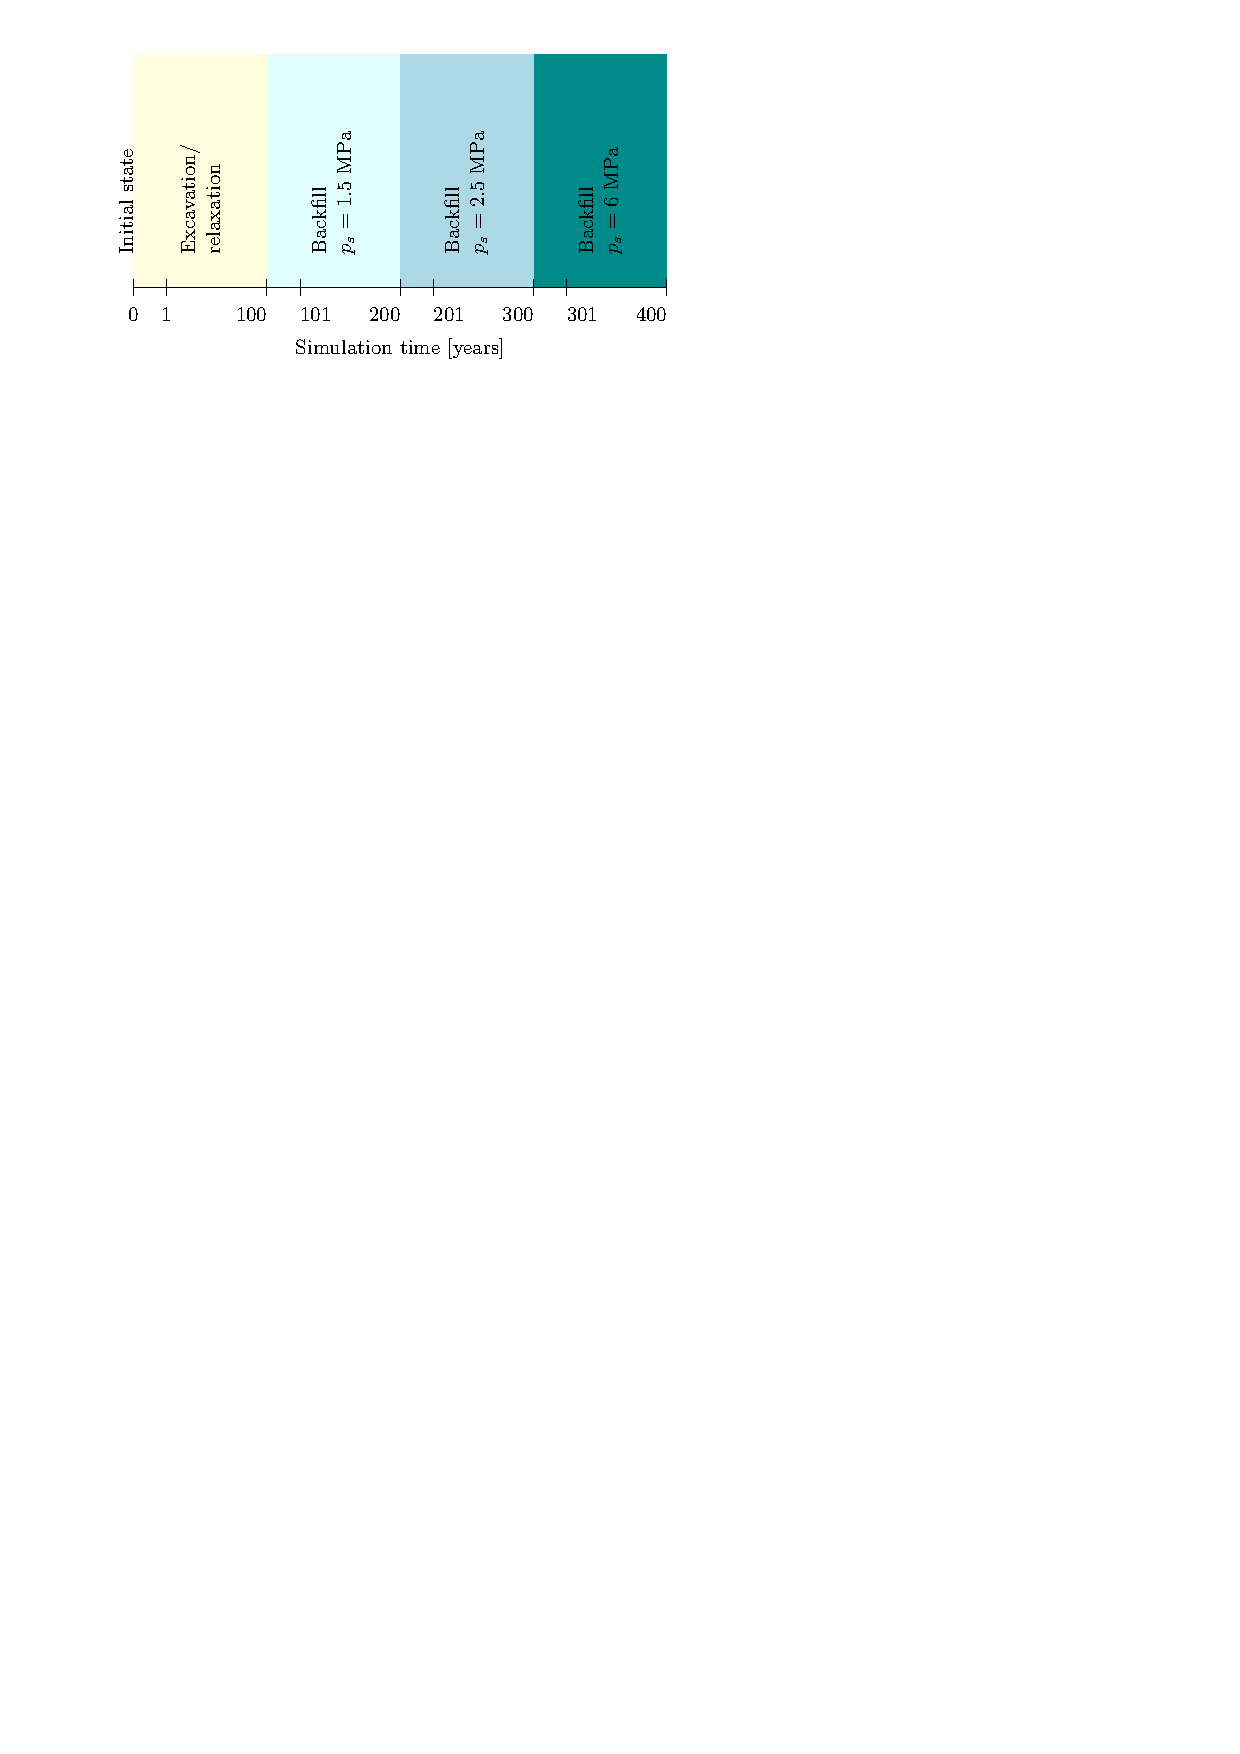
\includegraphics[width=0.75\textwidth]{graphics/hm_bentonit/time_points.pdf}
    \caption{HM model of storage facility: Simulation time interval and its division into epochs.}\label{fig:hm_bentonit_time}
\end{figure}

Two orientations of the access tunnel were considered, namely parallel and orthogonal to the direction of the maximal in-situ stress.

\subsection{Results and observations}

% We evaluate the change in principal rock parameters before and after filling by bentonite.

In the geometric configuration with the maximal in-situ stress in the direction of access tunnel, the following changes were observed:
\begin{itemize}
\item Hydraulic conductivity in the intact rock was \SI{2.94e-13}{\meter\per\second}.
After excavation, its values in the vicinity of the tunnel and the disposal wells  ranged between $[\num{9.1e-15}, \num{2.02e-11}]$ \unit{\meter\per\second}.
With bentonite backfill, the range progressively narrowed with increasing swelling pressure, ultimately reaching $[\num{9.83e-15}, \num{1.21e-11}]$ \unit{\meter\per\second}.
The highest conductivity was observed on the sides of the access tunnel; its value decreased by $40~\%$ due to backfilling.
We also examined values of hydraulic conductivity averaged through the direction of the tunnel axis. Using logarithmic mean values, the range was $[\num{1.14e-14}, \num{2.96e-12}]$ \unit{\meter\per\second}; with bentonite backfill this range narrowed to $[\num{1.59e-14}, \num{1.91e-12}]$ \unit{\meter\per\second}. The reduction in the maximum conductivity was then $35~\%$.

\item Piezometric head: After excavation, the range of the piezometric head was approximately $[-8,40]$ \unit\meter. During each backfilling epoch, the piezometric head gradually returned towards the initial value of 40 \unit{\meter}.

\item Displacement: The largest deformation changes occurred at the tunnel sides. The difference in displacement between excavated and backfilled states remained below 0.36 \unit{\milli\meter}.

\item Stress: The range of mean stress decreased with increasing swelling pressure. The maximum mean stress dropped from \SI{55.3}{\MPa} after excavation to \SI{49.9}{\MPa} at the end of simulation, corresponding to a reduction of $10~\%$.
Similarly the von Mises stress dropped from \SI{106}{\MPa} to \SI{81.9}{\MPa}, i.e. by $23~\%$.
\end{itemize}

When the orientation of the access tunnel is orthogonal to the maximal in-situ stress, a similar overall behaviour is observed, with some minor differences compared to the parallel case, which are highlighted below:
\begin{itemize}
\item Hydraulic conductivity ranges were approximately two orders of magnitude larger than in the parallel case. After excavation, the averaged values ranged between $\num{2.41e-14}$ and $\num{1.85e-10}]$ \unit{\meter\per\second}. 
With bentonite backfill, the range narrowed to $[\num{1.75e-14}, \num{1.19e-10}]$.
The maximum conductivity on the tunnel sides decreased by $35~\%$.

\item Piezometric head: The maximum value one year after excavation was higher, reaching $61$ \unit\meter. Otherwise, the response was qualitatively similar to that observed in the parallel case.

% \item Displacement: Highest deformation changes occur on tunnel sides. The difference in displacement between excavated and filled epoch are below 0.38 \unit{\milli\meter}.

\item Stress magnitudes were approximately twice as large as in the parallel configuration. The maximum mean stress decreased from \SI{117}{\MPa} after excavation to \SI{109}{\MPa} at the end of simulation, corresponding to a reduction of $7~\%$.
Similarly the von Mises stress dropped from \SI{235}{\MPa} to \SI{207}{\MPa}, i.e. by $12~\%$.
\end{itemize}

The described changes in principal fields are illustrated in Figures \ref{fig:range_conductivity}-\ref{fig:range_von_mises}.
In particular, Fig. \ref{fig:range_conductivity_box} shows the changes in the hydraulic conductivity during simulation epochs as well as the difference between the parallel and orthogonal case.
Similarly, Fig. \ref{fig:range_mean_stress_box} and \ref{fig:range_von_mises_box} depict the changes in the mean stress and the von Mises stress, respectively.

\begin{figure}
\centering
\begin{subfigure}{\textwidth}
    \centering
    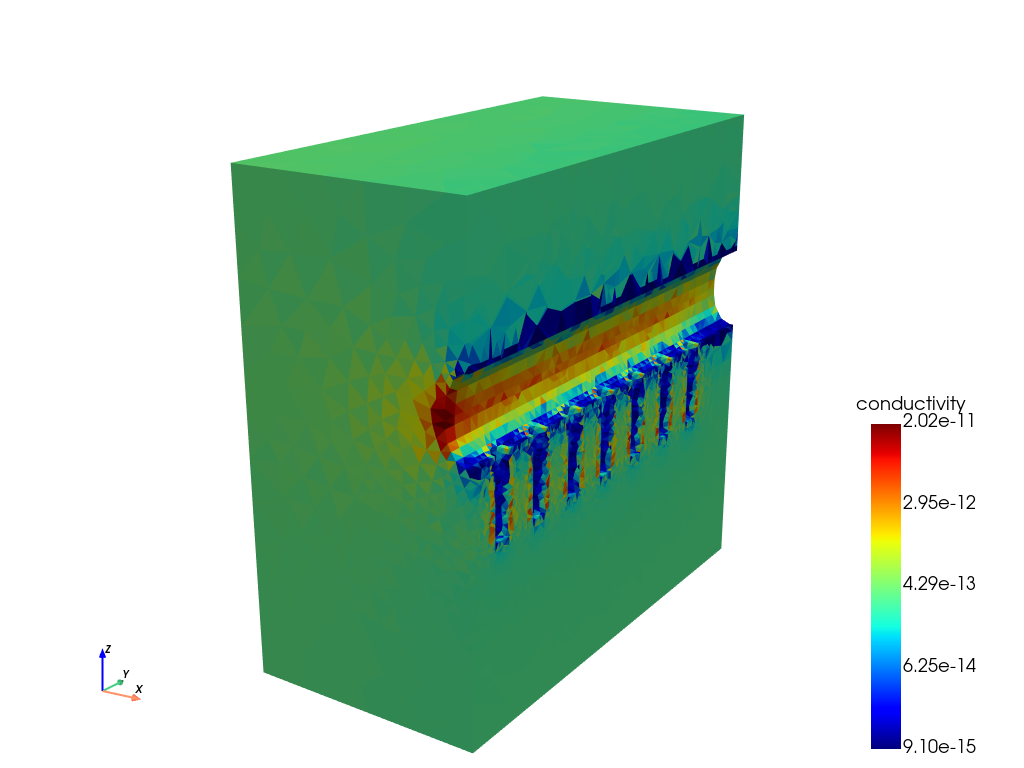
\includegraphics[width=0.49\textwidth]{graphics/hm_bentonit/parallel/plots/conductivity.100.0.png}
    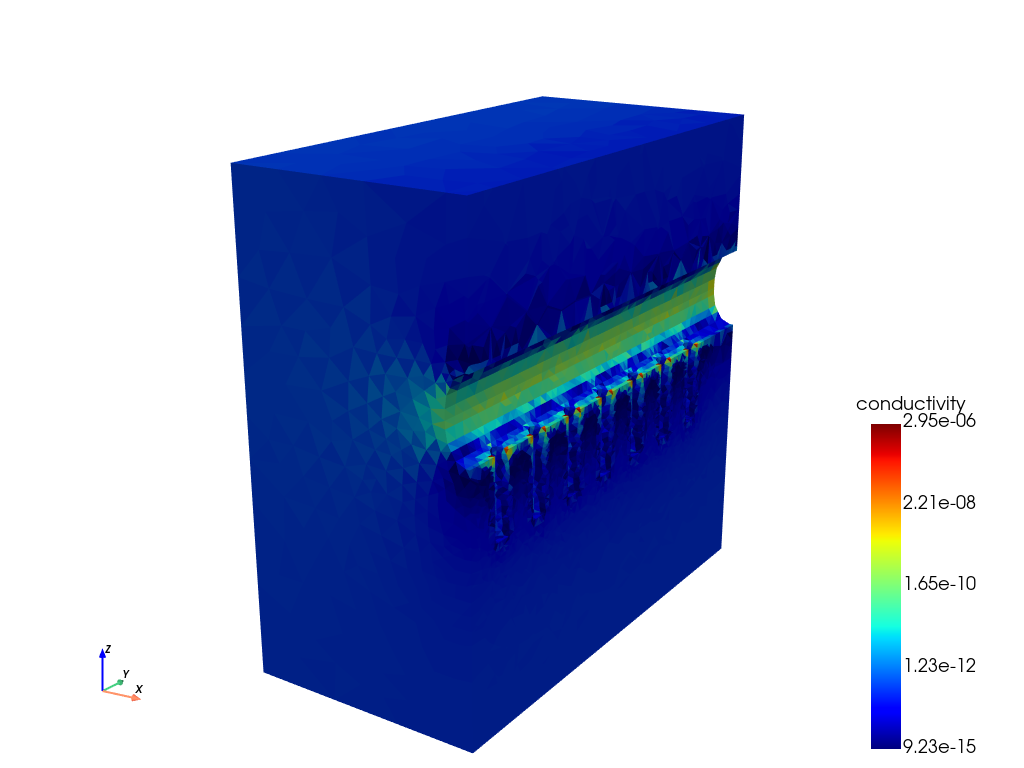
\includegraphics[width=0.49\textwidth]{graphics/hm_bentonit/orthogonal/plots/conductivity.100.0.png}
    \caption{Hydraulic conductivity 1 year after excavation. Left: parallel case; Right: orthogonal case.}
\end{subfigure}
\begin{subfigure}{\textwidth}
    \centering
    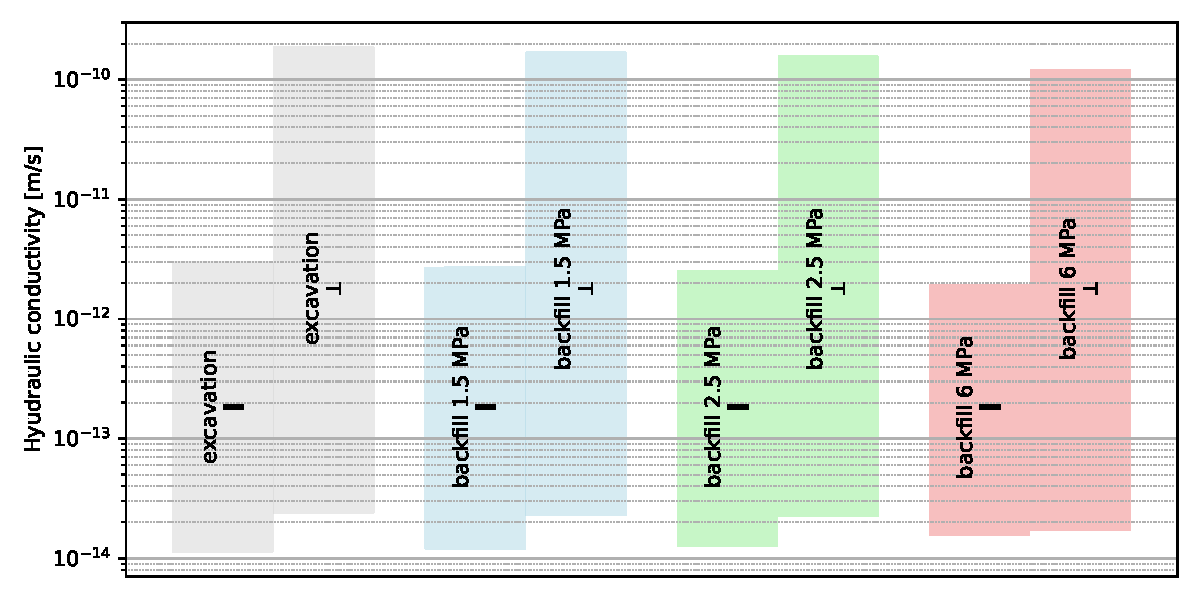
\includegraphics[width=\textwidth]{graphics/hm_bentonit/box_ranges/conductivity slice.box.pdf}
    \caption{Range of hydraulic conductivity during simulation epochs ($\parallel$ - parallel case, $\perp$ - orthogonal case). The ranges were taken from averaged values along the tunnel axis.}\label{fig:range_conductivity_box}
\end{subfigure}
\caption{Hydraulic conductivity: comparison of parallel and orthogonal orientation of the tunnel with respect to the direction of maximal in-situ stress.}\label{fig:range_conductivity}
\end{figure}

\begin{figure}
\centering
\begin{subfigure}{\textwidth}
    \centering
    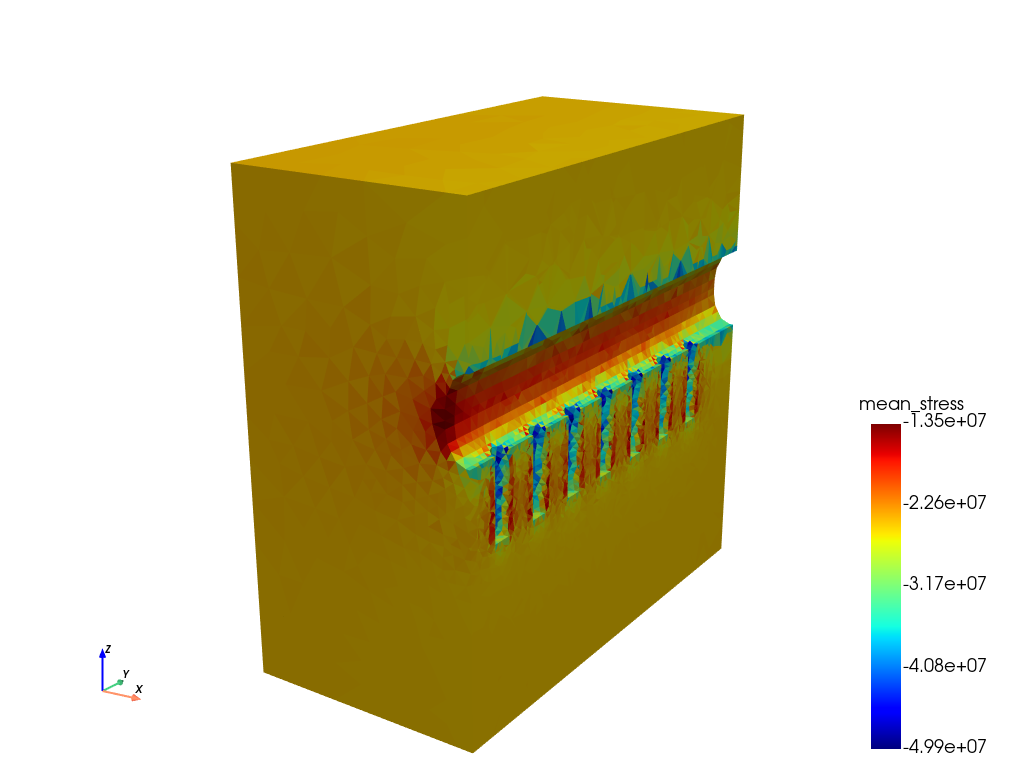
\includegraphics[width=0.49\textwidth]{graphics/hm_bentonit/parallel/plots/mean_stress.400.0.png}
    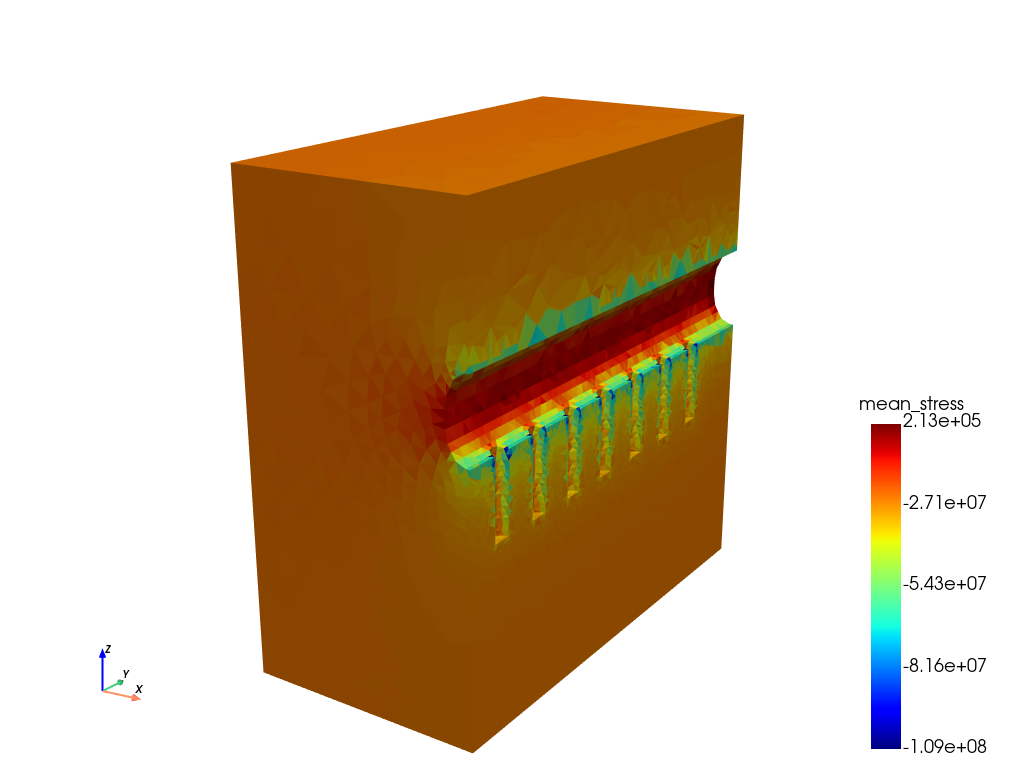
\includegraphics[width=0.49\textwidth]{graphics/hm_bentonit/orthogonal/plots/mean_stress.400.0.png}
    \caption{Mean stress at final state ($p_s=6$ \unit\MPa). Left: parallel case; Right: orthogonal case.}
\end{subfigure}
\begin{subfigure}{\textwidth}
    \centering
    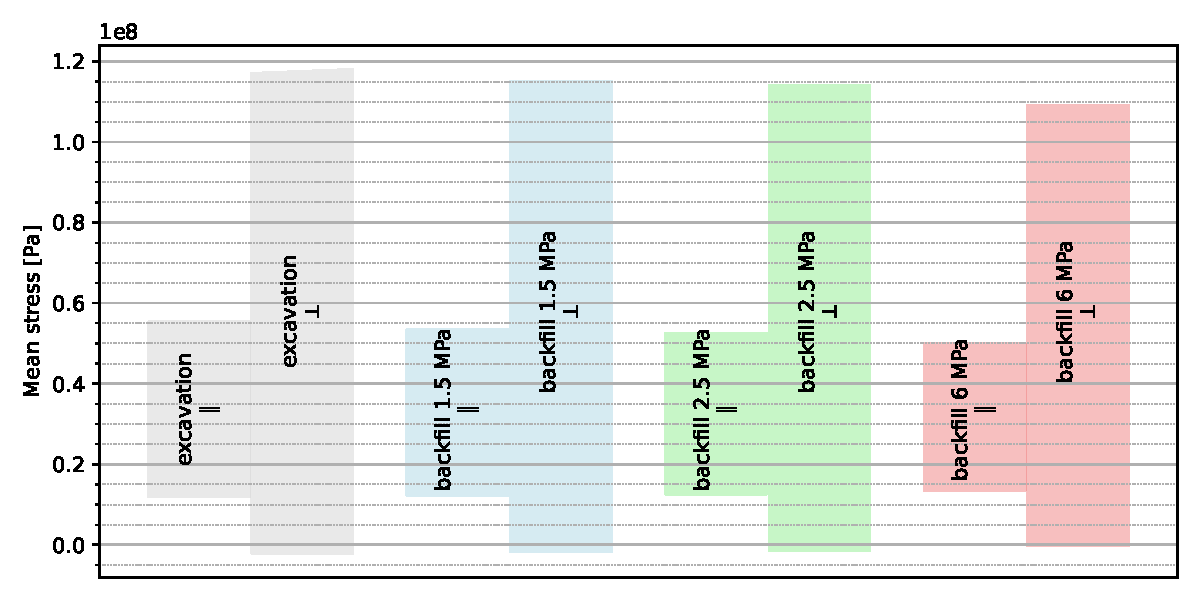
\includegraphics[width=\textwidth]{graphics/hm_bentonit/box_ranges/mean stress.box.pdf}
    \caption{Range of mean stress during simulation epochs ($\parallel$ - parallel case, $\perp$ - orthogonal case).}\label{fig:range_mean_stress_box}
\end{subfigure}
\caption{Mean stress: comparison of parallel and orthogonal orientation of the tunnel with respect to the direction of maximal in-situ stress.}\label{fig:range_mean_stress}
\end{figure}

\begin{figure}
\centering
\begin{subfigure}{\textwidth}
    \centering
    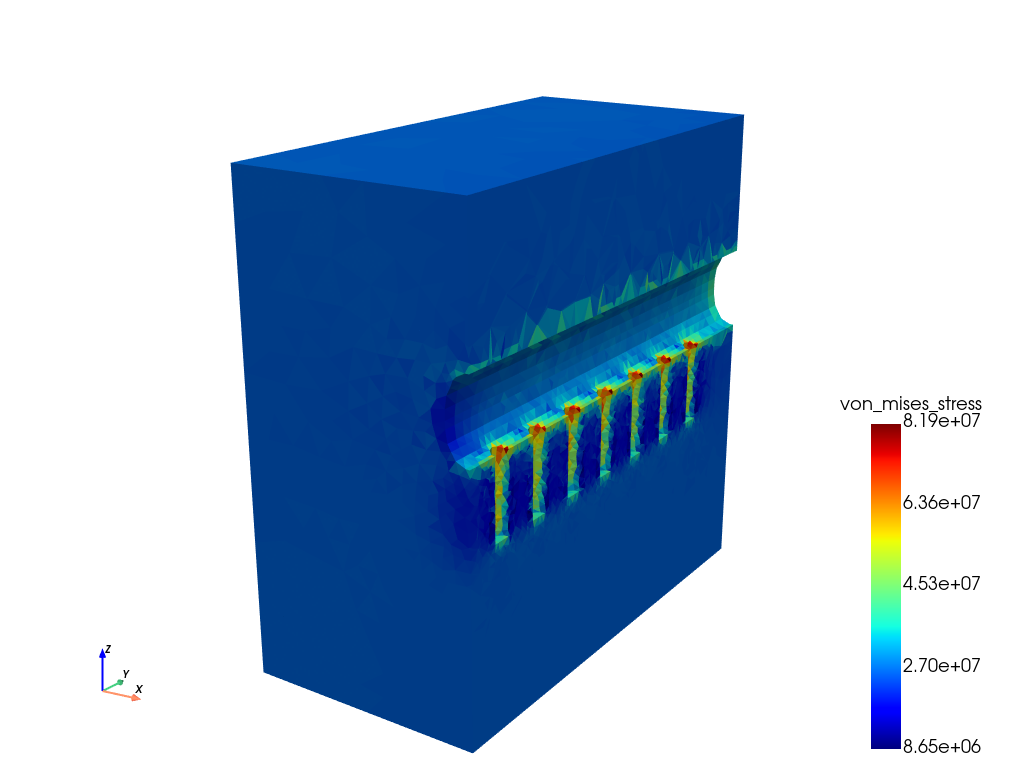
\includegraphics[width=0.49\textwidth]{graphics/hm_bentonit/parallel/plots/von_mises_stress.400.0.png}
    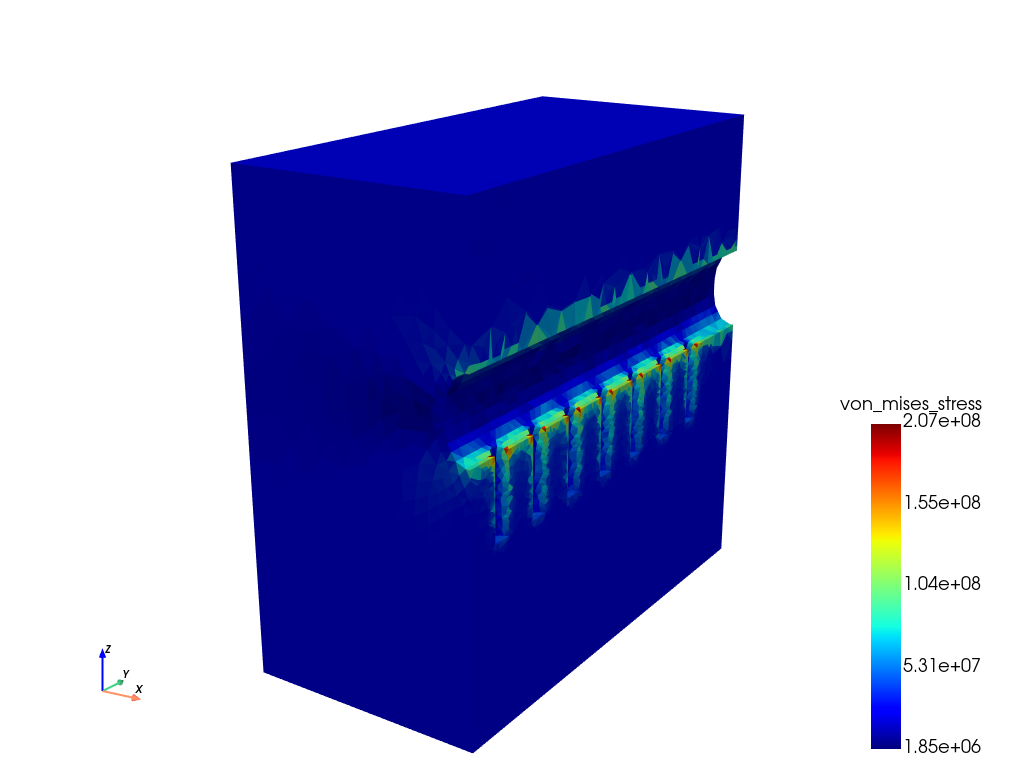
\includegraphics[width=0.49\textwidth]{graphics/hm_bentonit/orthogonal/plots/von_mises_stress.400.0.png}
    \caption{Von Mises stress at final state ($p_s=6$ \unit\MPa). Left: parallel case; Right: orthogonal case.}
\end{subfigure}
\begin{subfigure}{\textwidth}
    \centering
    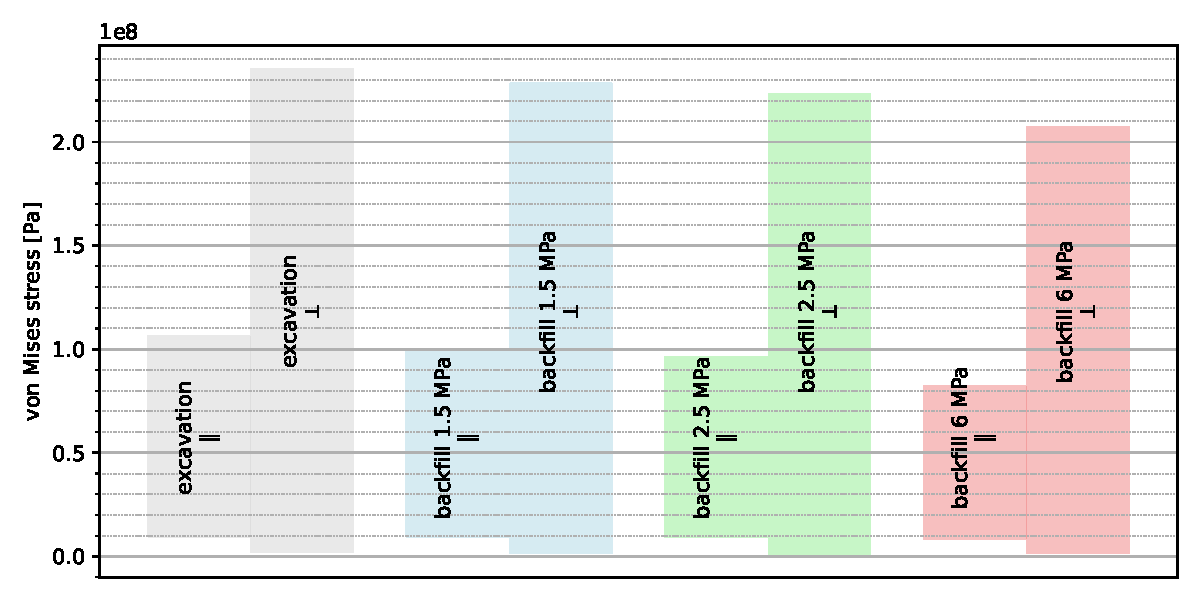
\includegraphics[width=\textwidth]{graphics/hm_bentonit/box_ranges/von mises stress.box.pdf}
    \caption{Range of von Mises stress during simulation epochs ($\parallel$ - parallel case, $\perp$ - orthogonal case).}\label{fig:range_von_mises_box}
\end{subfigure}
\caption{Von Mises stress: comparison of parallel and orthogonal orientation of the tunnel with respect to the direction of maximal in-situ stress.}\label{fig:range_von_mises}
\end{figure}




\section{Sensitivity analysis}
\label{sec:sensitivity}

This section introduces the grouped Sobol framework used for the sensitivity analysis, then specifies the stochastic distributions of the model parameters, and finally interprets the simulation results. In the results part, we first summarize transport features common to all cases, namely the role of dispersion and the advection-to-diffusion balance, and only then discuss the individual case studies.

\subsection{Variance-based sensitivity analysis}
Our quantity of interest (QoI) $Y$ is the safety indicator produced deterministically by the transport model.
Hence, $Y=f(\mathbf{X})$ is a function of the uncertain model parameters $\mathbf{X}=(X_1,\dots,X_D)$.
Assuming independence of the input parameters, the total variance of $Y$ can be decomposed into contributions
caused by individual parameters and by their interactions.

Importantly, variance-based sensitivity analysis does \emph{not} require any smoothness or continuity of $f$.
This allows us to use a single parameter as a seed for a pseudo-random generator and, in this way, generate
a (high-dimensional) vector of random inputs. We can then quantify the aggregate impact of uncertainty coming
from this parameter group. Ultimately, such a vector may represent one realization of an entire random fracture
network or a random field, i.e.\ a~representation of aleatory uncertainty.

\paragraph{ANOVA variance decomposition.}
Under the independence assumption, the Hoeffding--Sobol (functional ANOVA) decomposition holds in $L^2$:
\begin{equation}
f(\mathbf{X}) = f_0 + \sum_{i=1}^D f_i(X_i) + \sum_{1\le i<j\le D} f_{ij}(X_i,X_j) + \cdots + f_{1\cdots D}(X_1,\dots,X_D),
\end{equation}
with $f_0=\mathbb{E}[Y]$ and orthogonality conditions ensuring uniqueness, e.g.
$\mathbb{E}[f_u(\mathbf{X}_u)\,|\,X_k]=0$ for any $k\in u$. Consequently, the variance decomposes as
\begin{equation}
\Var(Y) = \sum_{i=1}^D V_i + \sum_{1\le i<j\le D} V_{ij} + \cdots + V_{1\cdots D},
\end{equation}
where $V_u=\Var\!\big(f_u(\mathbf{X}_u)\big)$ is the partial variance contributed by the subset $u\subseteq\{1,\dots,D\}$.

\paragraph{Sobol sensitivity indices: definitions and interpretation.}
The \emph{first-order} (main-effect) Sobol index of $X_i$ measures the fraction of output variance explained by varying
$X_i$ alone:
\begin{equation}
S_i = \frac{V_i}{\Var(Y)}.
\end{equation}
The \emph{second-order} index quantifies the additional variance due to interaction between $X_i$ and $X_j$ beyond their main effects:
\begin{equation}
S_{ij} = \frac{V_{ij}}{\Var(Y)}.
\end{equation}
The \emph{total-effect} index measures the overall contribution of $X_i$, including all its interactions with other inputs:
\begin{equation}
S_{T_i} = \frac{\sum_{u\ni i} V_u}{\Var(Y)},
\end{equation}
The exact indices satisfy inequalities:
$0\le S_i\le S_{T_i}\le 1$, and
\begin{equation}
\sum_{i=1}^D S_i \le 1.
\end{equation}
In particular, $S_{T_i}-S_i$ is a useful diagnostic of how
strongly $X_i$ interacts with other parameters. If $S_{T_i}$ is small, then $X_i$ can often be fixed (or simplified) with minimal impact on $\Var(Y)$. Higher-order indices, while theoretically possible, are usually not considered in practice because they are prohibitively computationally demanding.

\paragraph{Estimation of Sobol indices and computational cost.}
Sobol indices are typically estimated by Monte Carlo sampling. A common choice is the Saltelli sampling scheme \cite{Saltelli_Variance_2010} based on two
independent sampling matrices $A,B\in\mathbb{R}^{N\times D}$ and $D$ \textquote{mixed} matrices $A_B^{(i)}$ obtained by replacing the
$i$-th column of $A$ with the $i$-th column of $B$. This leads to a structured set of model evaluations of size
\begin{equation}
N \times (2D+2).
\end{equation}
In practice, one often takes $N\gtrsim 10^3$ to obtain sufficient precision for the dominant indices, whereas
substantially larger $N$ may be needed to estimate second-order indices reliably.

In our computations, a \emph{single} full model evaluation takes about $30$ minutes. For $D=6$ parameters, the full Saltelli
design therefore requires tens of thousands of model evaluations, which in our case translates into approximately one day on
$400$ CPUs. This cost makes a naive extension to many more parameters infeasible.



\paragraph{Towards reduced computational complexity.}
To make the approach tractable, we group inputs into a small number of physically meaningful parameter groups and compare the variance
contributions \emph{between groups} (grouped Sobol indices), rather than attempting to resolve all individual parameters at once.

Unfortunately the standard surrogate-model acceleration techniques (e.g.\ polynomial chaos expansions) are not directly applicable 
due to highly non-smooth and convoluted nature of the model function $f(\vc X)$ due to aleatory uncertainty encoded via pseudo-random seeds.

To reduce the cost of sensitivity analysis by at least two orders of magnitude, we are developing variance-reduction and
multi-fidelity strategies, in particular numerical homogenization ideas \cite{Spetlik_Convolutional_2026} and multi-level Monte Carlo (MLMC) estimators \cite{Giles2015}.

\subsection{Stochastic model parameters}
% The following summary is based on the data from technical reports of SÚRAO from several research projects studying \URFBII.

\subsubsection{Types of parameter distributions}
To describe the distributions of the independent model parameters $X_i$, we specify a probability distribution for each parameter. Where applicable, each distribution is characterized by
(i) a \emph{location} parameter (e.g. a mean) that sets the typical magnitude of sampled values, and
(ii) an \emph{uncertainty scale} parameter (e.g., a standard deviation) that quantifies sample variability.
We use following four distribution types.

\paragraph{Lognormal distribution}
Many transport-model parameters (e.g., hydraulic conductivity, diffusivity, \dots) are assumed to be lognormally distributed.
For lognormal variables, the arithmetic mean and standard deviation are often not the most informative descriptors.
Following previous work \cite{tz_design}, we therefore use the geometric mean \Gls{GM} as the location parameter,
which has the same physical unit as the quantity $Q$:
\[
\gm(Q) = \exp\!\Big(\mathrm{mean}\big(\log(Q)\big)\Big).
\]
As an uncertainty descriptor, we use the confidence-interval factor \Gls{CIF}:
\[
\cif(Q) = \exp\!\Big(3 \cdot \std\big(\log(Q)\big)\Big).
\]
The \Gls{CIF} admits a convenient interpretation: the (approximate) $99~\%$ confidence interval of $Q$ is
\[
\conf(Q,99\%) \approx \gm(Q)\,\Big[\cif^{-1}(Q),\, \cif(Q)\Big].
\]

\paragraph{Truncated normal distribution}
Porosity is modeled using a truncated normal distribution with mean as the location parameter,  a truncation interval $(q_{\min}, q_{\max})$, and standard deviation as the scale parameter.
All distribution parameters have the same unit as the modeled quantity.

\paragraph{Bayesian posterior distribution}
The parameters $(p_{30}, m, \alpha)$ of the DFN fracture families are not independent and are therefore sampled jointly.
We draw these parameters as tuples from the empirical population of posterior samples obtained by Bayesian inversion.
Hence, the distribution is represented by this finite set of samples.


\paragraph{Seed}
Aleatory uncertainties (fracture-network realization and computational mesh generation) are represented via the seed of a
pseudorandom number generator driving the corresponding random processes.
The seed is obtained by applying a hash function to a random value drawn from the uniform distribution on $(0,1)$.
The hash is applied to decorrelate the seed from the raw sample value produced by the same pseudorandom generator, ensuring reproducible yet effectively independent realizations.

%JB: continue here

\subsubsection{Model parameter distributions}

\paragraph{Aleatory parameters}
The transport model (Section~\ref{sec:transport_model}) is subject to two sources of aleatory uncertainty:
(i) the random discrete-fracture network, representing geological uncertainty, and
(ii) numerical uncertainty arising from the construction of the computational mesh.

For simplicity, we neglect spatial heterogeneity of the material parameters (caused by unresolved small-scale fractures). We therefore use spatially constant material parameters, with variability inferred from the observed in-situ spatial variability. This choice likely overestimates the sensitivity to these parameters, because true spatial variability would be partly smoothed by diffusive transport processes and mixing. Other sources of numerical uncertainty (e.g., time stepping and numerical diffusion) are neglected; based on numerical experiments, their contribution appears to be small.


\paragraph{DFN parameters}
The DFN is represented by five fracture families, with parameters inferred from mapping of fracture outcrops on the excavation walls at \URFB, as described in \cite{ZunaEtal2024FractureConnectivityBukovURF}.
Bayesian inversion was used to obtain joint posterior distributions of the fracture-size parameters $(p_{30}, \alpha)$.
The posterior samples (as yet unpublished) provided by Tomáš Janda and Petr Kabele (ČVUT) are shown in Figure~\ref{fig:fr_size_distr}.

\begin{table}[ht]
    \caption{Fisher distribution parameters of fracture populations.}
    \label{tab:fisher_params}  
    \centering
    \begin{tabular}{crrrrr}
    \toprule
    Population & Dip $\bunit{^o}$ & Strike $\bunit{^o}$ & Concentration & $r_{min}$ $\bunit{m}$ & $r_{max}$ $\bunit{m}$\\
    \midrule
    1 & 85.319 & 97.048  & 18.348 & 0.531 & 500 \\
    2 & 23.856 & 28.219  & 12.967 & 0.614 & 500 \\
    3 & 36.774 & 191.725 & 10.816 & 0.455 & 500 \\
    4 & 86.231 & 147.934 & 13.914 & 0.565 & 500 \\
    5 & 89.010 & 221.857 & 15.435 & 0.587 & 500 \\
    \bottomrule
    \end{tabular}
\end{table}

The Fisher-distribution parameters for fracture orientations were obtained using classical inversion.
The inferred orientation parameters are summarized in the Tab.~\ref{tab:fisher_params} and visualized in~\figref{fig:fr_fisher}.

Fracture aperture and hydraulic conductivity are related to the fracture size $r$ via \eqref{eq:k_frac} and \eqref{eq:k_frac_1}.
Since site-specific data are not available to calibrate the power-law parameters $a$ and $b$, we fix $b=3$ and use a common distribution of $a$
for all five fracture families. The geometric mean and variance of $a$ are derived from repository-scale values reported in \cite{Ohman_Site_2010}.
A summary of the DFN parameters is given in Table~\ref{tab:param_dfn_edz}.



\begin{figure}[!htb]
     \centering
     \begin{subfigure}[b]{0.325\textwidth}
         \centering
         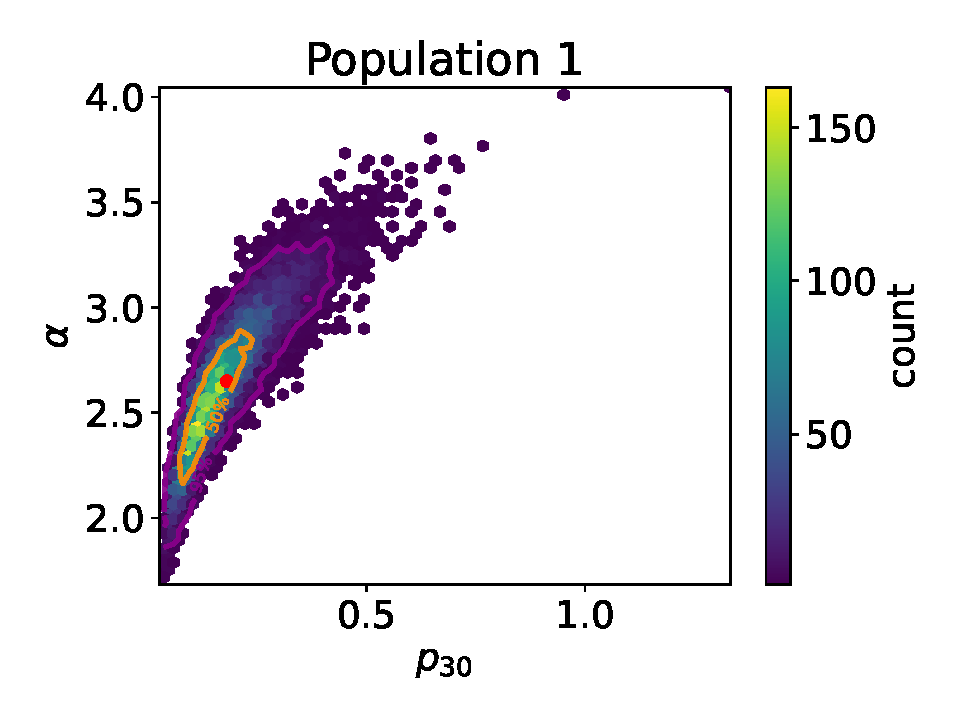
\includegraphics[width=\textwidth]{graphics_tr/fr_pop_1.pdf}
         % \caption{$y=x$}
         % \label{fig:y equals x}
     \end{subfigure}
     \hfill
     \begin{subfigure}[b]{0.325\textwidth}
         \centering
         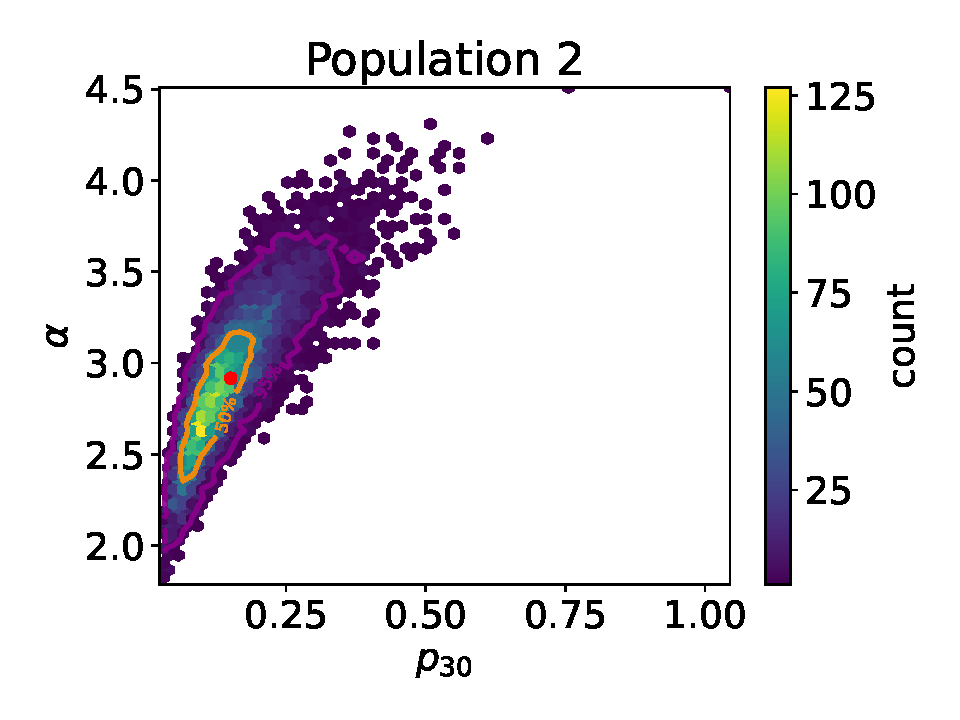
\includegraphics[width=\textwidth]{graphics_tr/fr_pop_2.pdf}
         % \caption{$y=3\sin x$}
         % \label{fig:three sin x}
     \end{subfigure}
     \hfill
     \begin{subfigure}[b]{0.325\textwidth}
         \centering
         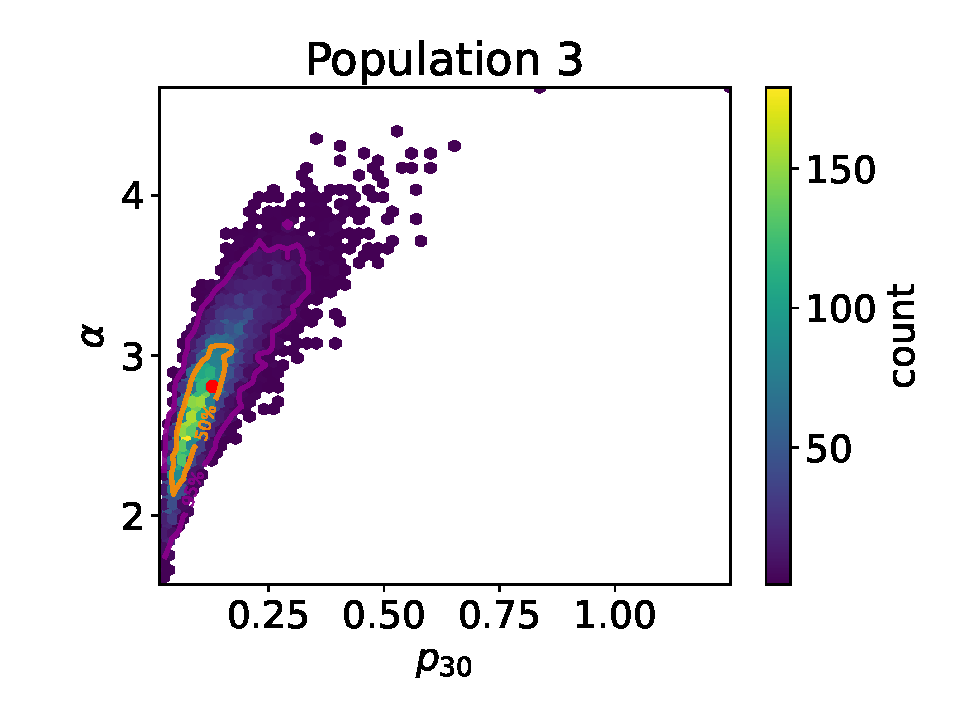
\includegraphics[width=\textwidth]{graphics_tr/fr_pop_3.pdf}
         % \caption{$y=5/x$}
         % \label{fig:five over x}
     \end{subfigure}

     \begin{subfigure}[b]{0.325\textwidth}
         \centering
         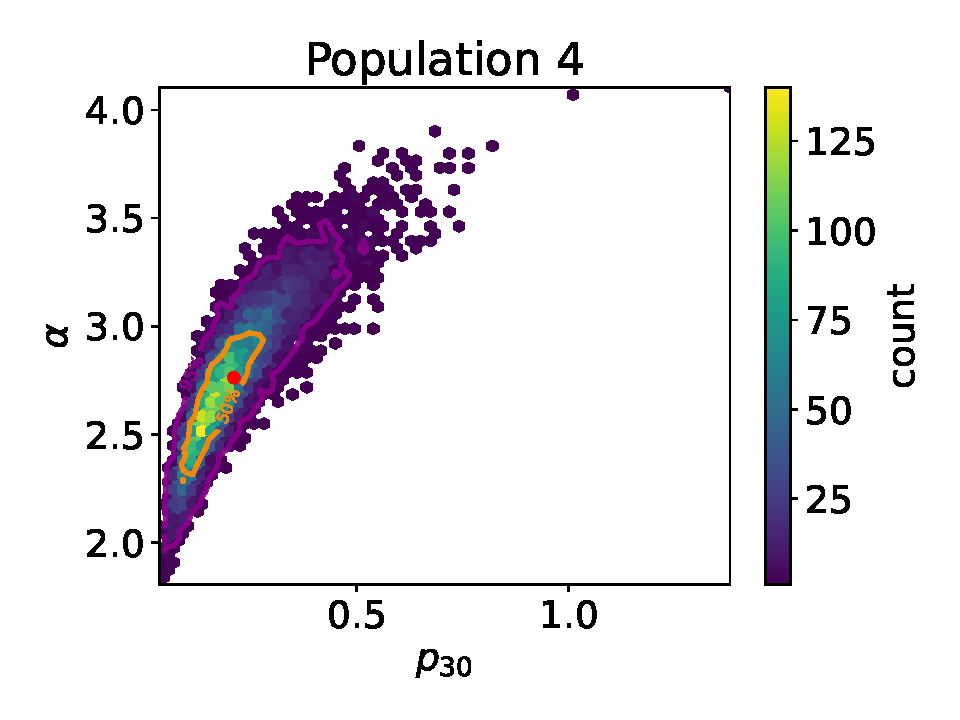
\includegraphics[width=\textwidth]{graphics_tr/fr_pop_4.pdf}
         % \caption{$y=x$}
         % \label{fig:y equals x}
     \end{subfigure}
     \hfil
     \begin{subfigure}[b]{0.325\textwidth}
         \centering
         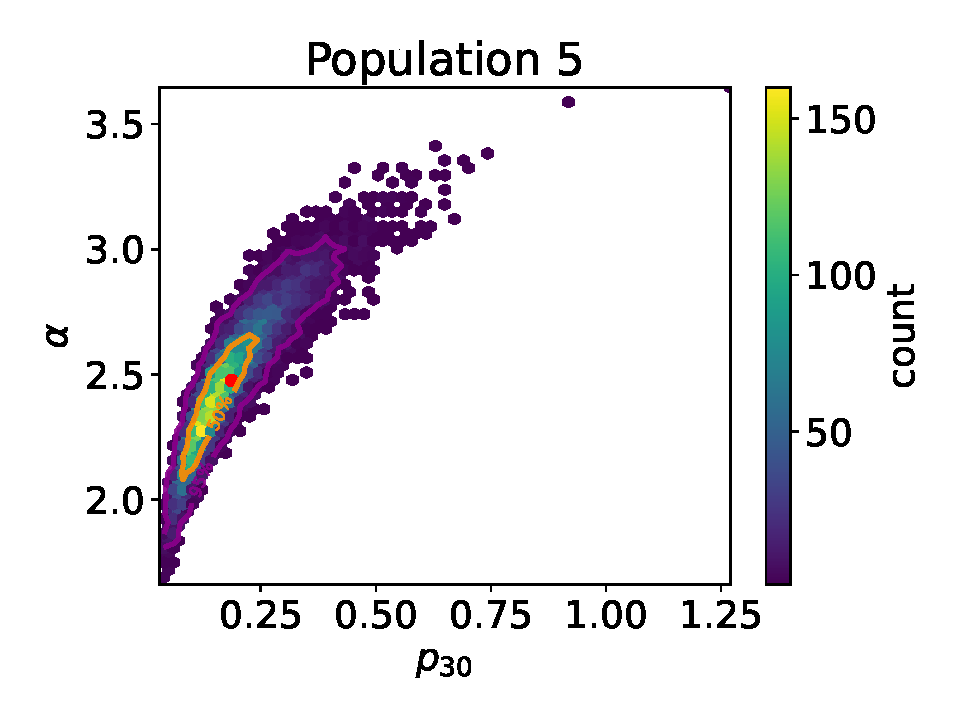
\includegraphics[width=\textwidth]{graphics_tr/fr_pop_5.pdf}
         % \caption{$y=3\sin x$}
         % \label{fig:three sin x}
     \end{subfigure}
        \caption{Posterior distributions of fracture size parameters $(p_{30}, \alpha)$ resulting from the Bayesian inversion per fracture population.}
        \label{fig:fr_size_distr}
\end{figure}



\begin{figure}[!htb]
     \centering
     \begin{subfigure}[b]{0.325\textwidth}
         \centering
         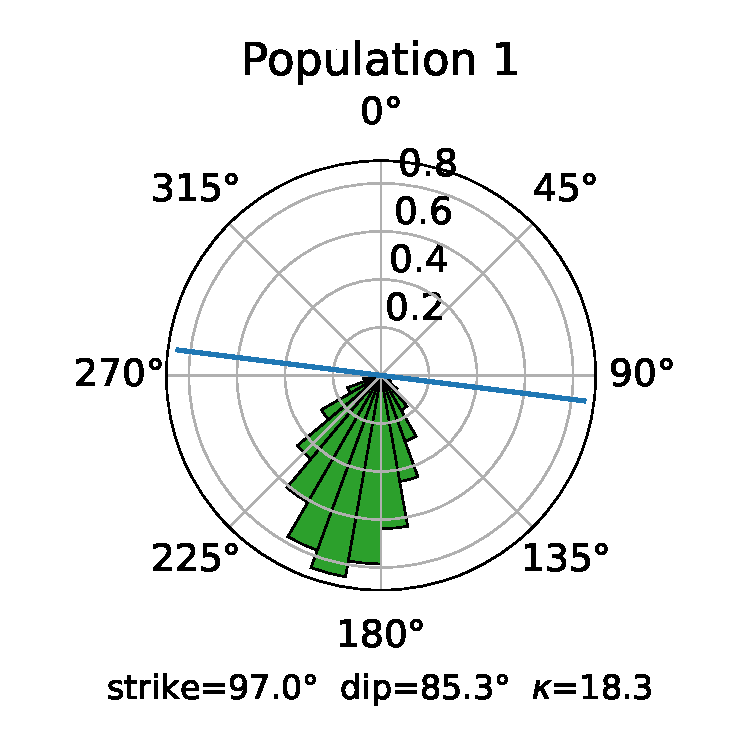
\includegraphics[width=\textwidth]{graphics_tr/fr_rose_1.pdf}
         % \caption{$y=x$}
         % \label{fig:y equals x}
     \end{subfigure}
     \hfill
     \begin{subfigure}[b]{0.325\textwidth}
         \centering
         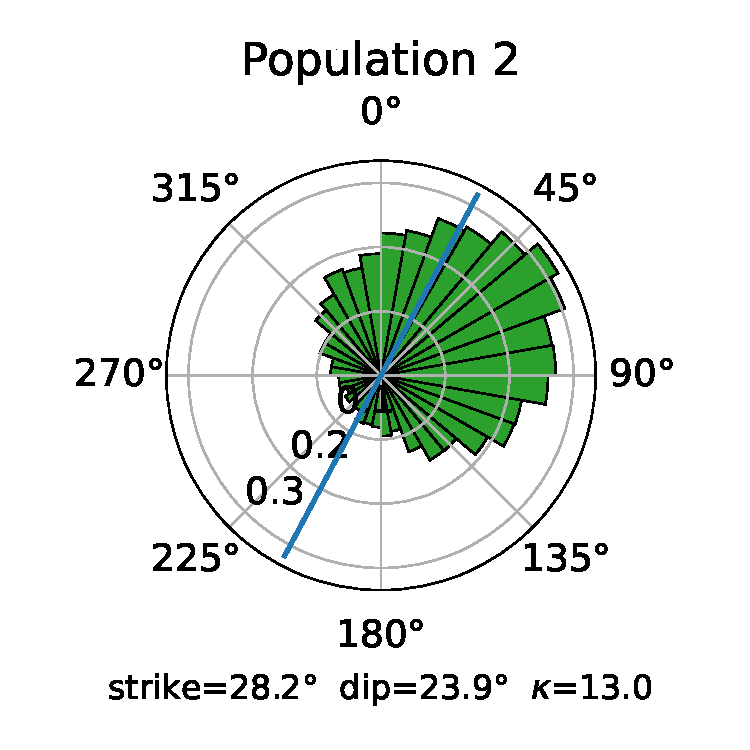
\includegraphics[width=\textwidth]{graphics_tr/fr_rose_2.pdf}
         % \caption{$y=3\sin x$}
         % \label{fig:three sin x}
     \end{subfigure}
     \hfill
     \begin{subfigure}[b]{0.325\textwidth}
         \centering
         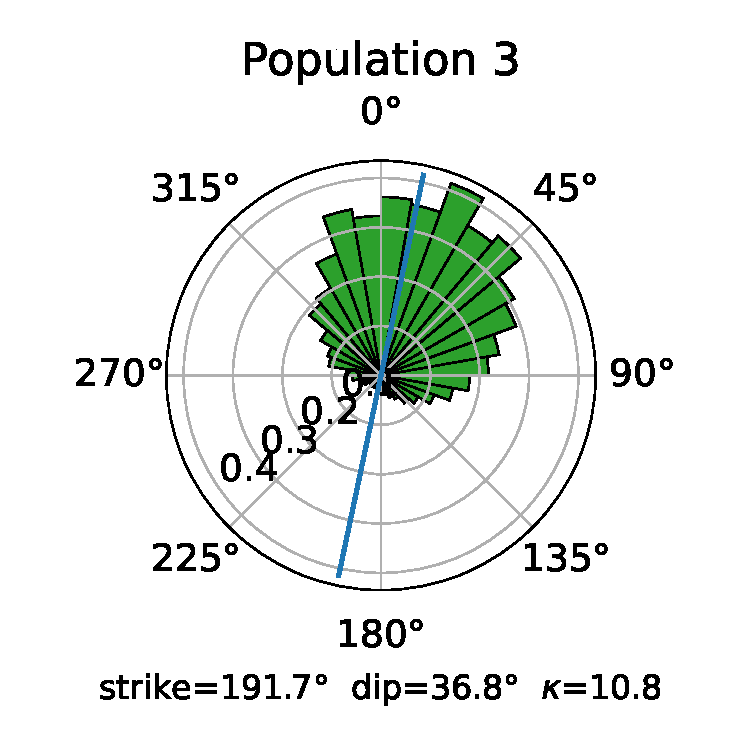
\includegraphics[width=\textwidth]{graphics_tr/fr_rose_3.pdf}
         % \caption{$y=5/x$}
         % \label{fig:five over x}
     \end{subfigure}

     \begin{subfigure}[b]{0.325\textwidth}
         \centering
         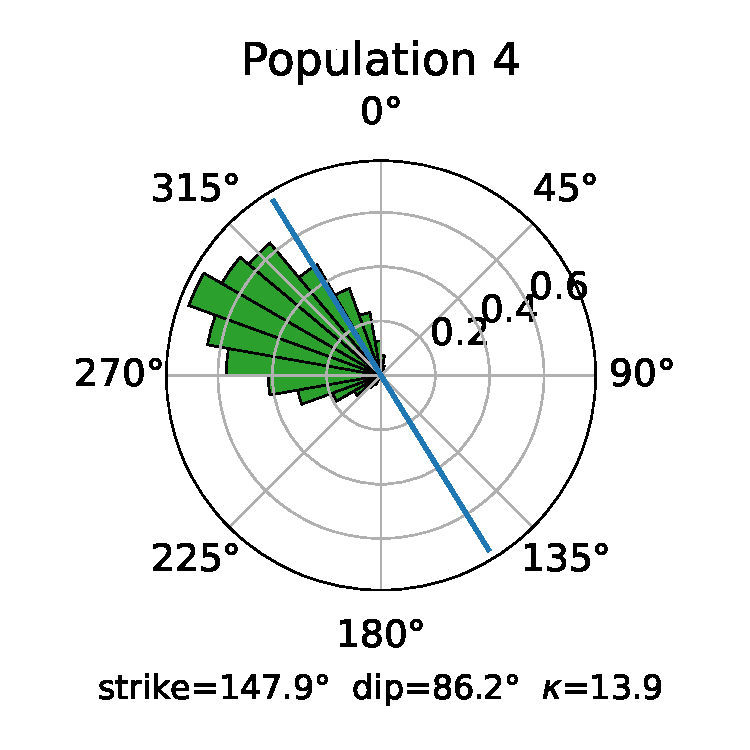
\includegraphics[width=\textwidth]{graphics_tr/fr_rose_4.pdf}
         % \caption{$y=x$}
         % \label{fig:y equals x}
     \end{subfigure}
     \hfil
     \begin{subfigure}[b]{0.325\textwidth}
         \centering
         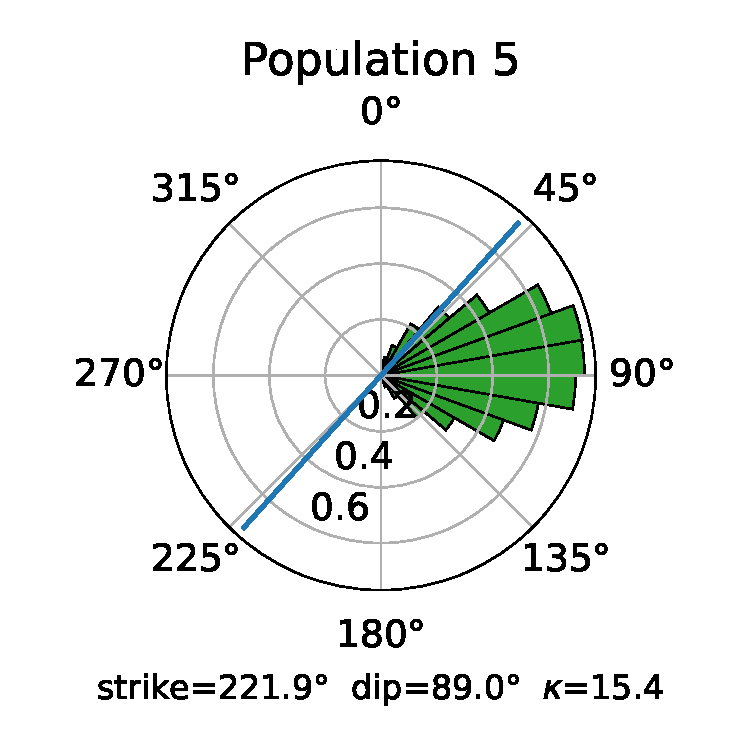
\includegraphics[width=\textwidth]{graphics_tr/fr_rose_5.pdf}
         % \caption{$y=3\sin x$}
         % \label{fig:three sin x}
     \end{subfigure}
        \caption{Strike rose diagrams of fracture orientation by von Mises-Fisher distribution per fracture population.}
        \label{fig:fr_fisher}
\end{figure}

\paragraph{EDZ parameters}
Based on the analysis in Section~\ref{sec:hm_steady}, we set the outer EDZ boundary to
$\edzRelThick = 1.5$--$2.5$ times the tunnel size. The conductivity scaling factor is sampled as
$\edzPerm \in [0.1,\,100]$ (see \figref{fig:range_conductivity_box}), and the porosity scaling factor as
$\edzPor \in [0.35,\,2.15]$.
A summary of the EDZ parameters is provided in Table~\ref{tab:param_dfn_edz}.

\paragraph{Matrix properties}
For both the backfill and rock-matrix domains, we prescribe hydraulic conductivity~$k$, porosity~$\theta$,
effective diffusion coefficient~$d_e$, and longitudinal dispersivity~$\alpha_L$.
For the backfill, mean values and sampling ranges are taken directly from Section~\ref{sec:transport_pellets}.
For diffusion, we use the mean value representative of neutral species and cations, while accounting for the larger
variability typical of anion-like tracers.

Rock-matrix properties are based on the review in Section~\ref{chapter:review}.
The conductivity distribution follows Section~\ref{sec:hydro_cond}, in particular the analysis of samples from borehole~V--12.
The porosity distribution spans the values reported in Section~\ref{sec:storativity}, and the effective diffusivity distribution
is based on measurements from borehole~V--12 samples reproduced in Section~\ref{sec:review_diffusion}.

The dispersivity distribution is derived from the relation $\alpha_L = I_h\,\Var(\ln K)$, consistent with the macrodispersivity model introduced in Section~\ref{sec:transport_pellets}, especially equation~\eqref{eq:dispersivity}.
% var(ln(k))=0.477 for std_log10(k)=0.3
The integral scale $I_h$ is sampled from $0.5$--$5\,\mathrm{m}$, ranging from the computational element size ($0.5\,\mathrm{m}$)
up to the characteristic size of the smallest discrete fractures ($5\,\mathrm{m}$).



\begin{table}[ht]
    \caption{Summary of DFN and EDZ parameters.}
    \label{tab:param_dfn_edz}
    \hfill
    \begin{minipage}[t]{0.45\textwidth}
        \centering
        \footnotesize
        \renewcommand{\arraystretch}{1.25}
        \begin{tabular}{ccccc}
        \toprule
        \multicolumn{5}{c}{DFN} \\
        \toprule
        $X^*$ & distr. & mean & unit & var \\
        \midrule
        $(p_{30}$, $\alpha)^{(i)}$ & Bayes & -- & -- & -- \\
        % mean_log10: -8.22, std_log10: 0.6
        %$a^{(i)}$ & logN & $0.6$& $\munit{m^2\cdot s^{-1}}$ & $63$ \\
        $a^{(i)}$ & logN & $6\cdot10^{-9}$& $\munit{m^2\cdot s^{-1}}$ & $63$ \\  
        % 9.3E-9 geometric mean of repository level values for 6 families in Ohman 2010
        % mean log_10 = -8.03, std log_10 = 0.61 ; there must be some confustion since this
        % match the values reported above.
        
        
        
        % $b^{(i)}$ & logN & $19$& MPa & $2.5$ \\
        $b^{(i)}$ & -- & $3$ & -- & -- \\
        \bottomrule
        \end{tabular}
        $^*$ We denote by $(\cdot)^{(i)}$ the parameters respective to one of the fracture population family, $i=0,\ldots,4$.
    \end{minipage}
    \hspace{2em}
    \begin{minipage}[t]{0.45\textwidth}
        \centering
        \footnotesize
        \renewcommand{\arraystretch}{1.25}
        \begin{tabular}{ccccc}
        \toprule
        \multicolumn{5}{c}{EDZ} \\
        \toprule
        $X$ & distr. & mean & unit & var \\
        \midrule
        \(\tilde{w}_e\) & tr. N & $2, [1.5,3]$ & -- & $0.15$ \\
        % mean_log10: 0.5, std_log10: 0.5
        \(\tilde k_e\) & logN & $3.16$ & -- & $31.6$ \\
        % 1.25, 0.3, 0.35, 2.15
        \(\tilde \theta_e\) & tr. N & $1.25, [0.35,2.15]$ & -- & $0.3$ \\
        \bottomrule
        \end{tabular}
    \end{minipage}
    \hfill
\end{table}

\begin{table}[ht]
    \caption{Summary of intact rock and bentonite backfill transport parameters.}
    \label{tab:param_matrix_backfill}
    \centering
    \begin{minipage}{0.44\textwidth}
        \centering
        \footnotesize
        \setlength{\tabcolsep}{4pt}
        \renewcommand{\arraystretch}{1.25}
        \begin{tabular}{@{}ccccc@{}}
        \toprule
        \multicolumn{5}{c}{Matrix} \\
        \toprule
        $X$ & dist. & mean & unit & var \\
        \midrule
        % mean_log10: -12.698970004336019, std_log10: 0.1
        $d_r$ & logN & $2 \cdot 10^{-13}$ & 
        $\munit{m^2\cdot s^{-1}}$ & $2.00$ \\
        % mean_log10: -12.522878745280337, std_log10: 0.3
        \(k_r\) & logN & $3 \cdot 10^{-13}$ & $\munit{m\cdot s^{-1}}$& $7.94$ \\
        % 0.008, 0.002, 0.001, 0.014
        \(\theta_r\) & tr. N & $0.008,\,[0.001,0.014]$ & -- & $0.002$ \\
        % mean_log10: -0.3010299956639812, std_log10: 0.15
        \(\alpha_{Lr}\) & logN & $0.5$ & $\munit{m}$ & $2.82$ \\
        \bottomrule
        \end{tabular}
    \end{minipage}
    \hfill
    \begin{minipage}{0.44\textwidth}
        \centering
        \footnotesize
        \setlength{\tabcolsep}{4pt}
        \renewcommand{\arraystretch}{1.25}
        \begin{tabular}{@{}ccccc@{}}
        \toprule
        \multicolumn{5}{c}{Backfill} \\
        \toprule
        $X$ & dist. & mean & unit & var \\
        \midrule
        % mean_log10: -11.0, std_log10: 0.3
        $d_b$ & logN & $10^{-11}$ & 
        $\munit{m^2\cdot s^{-1}}$ & $7.94$ \\
        % mean_log10: -12.397940008672037, std_log10: 0.26
        \(k_b\) & logN & $3\cdot10^{-13}$ & $\munit{m\cdot s^{-1}}$& $6.03$ \\
        % [0.51, 0.02, 0.45, 0.57]
        \(\theta_b\) & tr. N & $0.51,\,[0.45,0.57]$ & -- & $0.02$ \\
        % mean_log10: -1.08, std_log10: 0.15
        \(\alpha_{Lb}\) & logN & $0.083$ & $\munit{m}$ & $2.82$ \\
        \bottomrule
        \end{tabular}
    \end{minipage}

\end{table}





\FloatBarrier







%%%%%%%%%%%%%%
% TODO:
% - research of similar analysis
% - grafy: menší font popisků, sladit barvy, errorbars v grafech Sobol indexů
\subsection{Results}

\paragraph{Dispersion.}
The average velocities in the rock matrix and backfill are of the same order, $\sim 10^{-14}$, which corresponds to dispersivities of about $5\cdot 10^{-15}$ (rock matrix) and $8\cdot 10^{-16}$ (backfill). In the rock matrix, dispersion is roughly two orders of magnitude smaller than the effective diffusivity. 
Given that both parameters are uncertain, a non-negligible contribution from dispersion cannot be fully ruled out. Locally higher velocities may occur, in particular along \emph{matrix bridges} (short matrix connections between fractures).
In the backfill, by contrast, dispersion is about four orders of magnitude smaller than diffusivity, and large spatial variability in velocity or parameters is unlikely; its impact is therefore negligible.

\paragraph{Advection vs. diffusion.}
For an element length scale $L \approx 0.5\,\mathrm{m}$, the local Peclet number is
\[
\mathrm{Pe}=\frac{vL}{D_{\mathrm{eff}}}\approx \frac{(10^{-14})(0.5)}{5\cdot 10^{-13}} \approx 10^{-2}.
\]
This implies strongly diffusion-dominated transport ($\mathrm{Pe}\ll 1$) on the element scale in the rock matrix and, even more so, in the backfill. Locally higher velocities may occur (up to $10^{-11}$), in particular along matrix bridges and in major fractures, where advection may become more relevant.

\paragraph{Sensitivity analyses.}
We perform four global sensitivity analyses that differ in how the uncertain inputs are represented. Uncertainties are grouped by the part of the system they affect (bulk rock, backfill, EDZ, and the DFN when present). In addition to physical parameters, we treat the DFN realization (via a random DFN seed) and the computational mesh (via a random meshing seed) as aleatory sources of variability.

\emph{Case 0} is the reference setup and includes the DFN. 
\emph{Case 1} is a DFN-free control case (transport in matrix/backfill only), providing a conservative baseline. 
\emph{Case 2} follows \emph{Case 0} but refines the DFN-related grouping by separating geometric (population) and transport (transmissivity) parameters.
\emph{Case 3} follows \emph{Case 0} but assumes higher bulk-rock conductivity and dispersivity in order to represent the possible effect of unresolved small-scale fractures.

Because DFN realizations randomize the geometry, some runs fail during fracture-induced volume fragmentation, mesh generation, or the algebraic solve (slow convergence/divergence). Table~\ref{tab:sample_counts} reports the number of successful Saltelli samples and the corresponding wall time on 180 CPUs.

\begin{table}[ht]
    \caption{Sample count of computed cases.}
    \label{tab:sample_counts}
    \centering
    \footnotesize
    \renewcommand{\arraystretch}{1.25}
    \begin{tabular}{crcrr}
    \toprule
    Case & \makecell[c]{Saltelli\\ samples} & \makecell[c]{Parameter\\ groups} & \makecell[c]{Model\\ Evaluations} & Time [h:m] \\
    \midrule
    0 & 1497 / 2048 & 6 & 27132 / 28672 & 60:01\\
    1 & 2038 / 2048 & 4 & 20470 / 20480 & 10:42\\
    2 & 1495 / 2048 & 6 & 27123 / 28672 & 70:10\\
    3 & 755 / 1024 & 6 & 13590 / 14336 & 47:10\\
    \bottomrule
    \end{tabular}
\end{table}


%%%%%% Case 00
%%%%%%%%%%%%%%%%%%%%%%%%%%%%%%%%%%%%%%%%%%%%%%%%%%%%%%%%%%%%
\FloatBarrier
\subsubsection{Case 0}
The reference case comprises six parameter groups representing the main sources of uncertainty:
\begin{enumerate}
    \item bulk rock: $k_r$, $\theta_r$, $d_r$, $\alpha_{Lr}$
    \item backfill: $k_b$, $\theta_b$, $d_b$, $\alpha_{Lb}$
    \item EDZ: $\tilde k_e$, $\tilde \theta_e$, $\tilde w_e$
    \item DFN parameters: $(p_{30}, \alpha)^{(i)}$, $a^{(i)}$
    \item DFN realization (seed)
    \item meshing seed
\end{enumerate}


\figref{fig:case_00_conc} summarizes the time evolution of the \gls{QoI} $I(t)$ (defined in Section~\ref{sec:QoI}). The top panel shows selected quantiles together with an estimated probability density function (PDF). The bottom panel shows the 20 lowest (red) and 20 highest (blue) trajectories, overlaid with a colormap representation of the PDF for a tightened range of the log concentrations. The breakthrough time is on the order of $2\,\munit{ky}$, but varies widely—from about $0.11\,\munit{ky}$ to several $100\,\munit{ky}$. The peak concentration reaches approximately $\num{1e-6}$. At $t=10\,\munit{ky}$, the concentration spans roughly ten orders of magnitude across samples, whereas by the final time ($640\,\munit{ky}$) the spread narrows to about two orders of magnitude. A similar level of variability is observed for the maximum concentration over time.


The estimated Sobol indices produced by the sensitivity analysis are displayed in \figref{fig:case_00_sobol}. 
Reading the figure from right to left, the total-effect indices (ST) for the aggregated quantity $\max I(t)$ 
identify two dominant sources of uncertainty: the \gls{DFN} parameter group and the particular \gls{DFN} realization. A smaller additional contribution is associated with meshing; however, its first-order effect is negligible, its S2 estimates have large error bars, and its apparent importance decreases as the number of samples increases. 

For the aggregated quantity $\max I(t)$, the only clearly significant first-order contribution is the \gls{DFN} seed, while the S1 index of the \gls{DFN} parameter group is the second largest but only marginally significant. The corresponding second-order indices remain too uncertain for firm conclusions, although they suggest a possible interaction between the bulk-rock, bentonite, and \gls{EDZ} material groups.

The time-dependent Sobol indices indicate a marked change after about $100\,\munit{ky}$, when the \gls{QoI} in the majority of realizations has already approached its late-time tail regime. At late times, the set of indices selected as significant for the aggregated QoI drops toward zero and may even attain negative estimates due to sampling error. This effect is most likely caused by sampling error, since it does not appear in Case~2, which has an almost identical parameterization. The time-resolved plot further suggests interaction of the \gls{DFN} seed with all three material groups, whereas the \gls{DFN} parameter group does not show a similarly clear interaction with the backfill material group within the present estimation accuracy.


% Decreasing the uncertainty in DFN parameters is the only option. However, fitting DFN parameters to the larger datasets of outcrops may be counterproductive, better analysis of the outcrop dataset must be performed to decide whether the uncertainty is primarily epistemic, space variability or truly aleatory.

    
\begin{figure}[!htb]
    \centering
    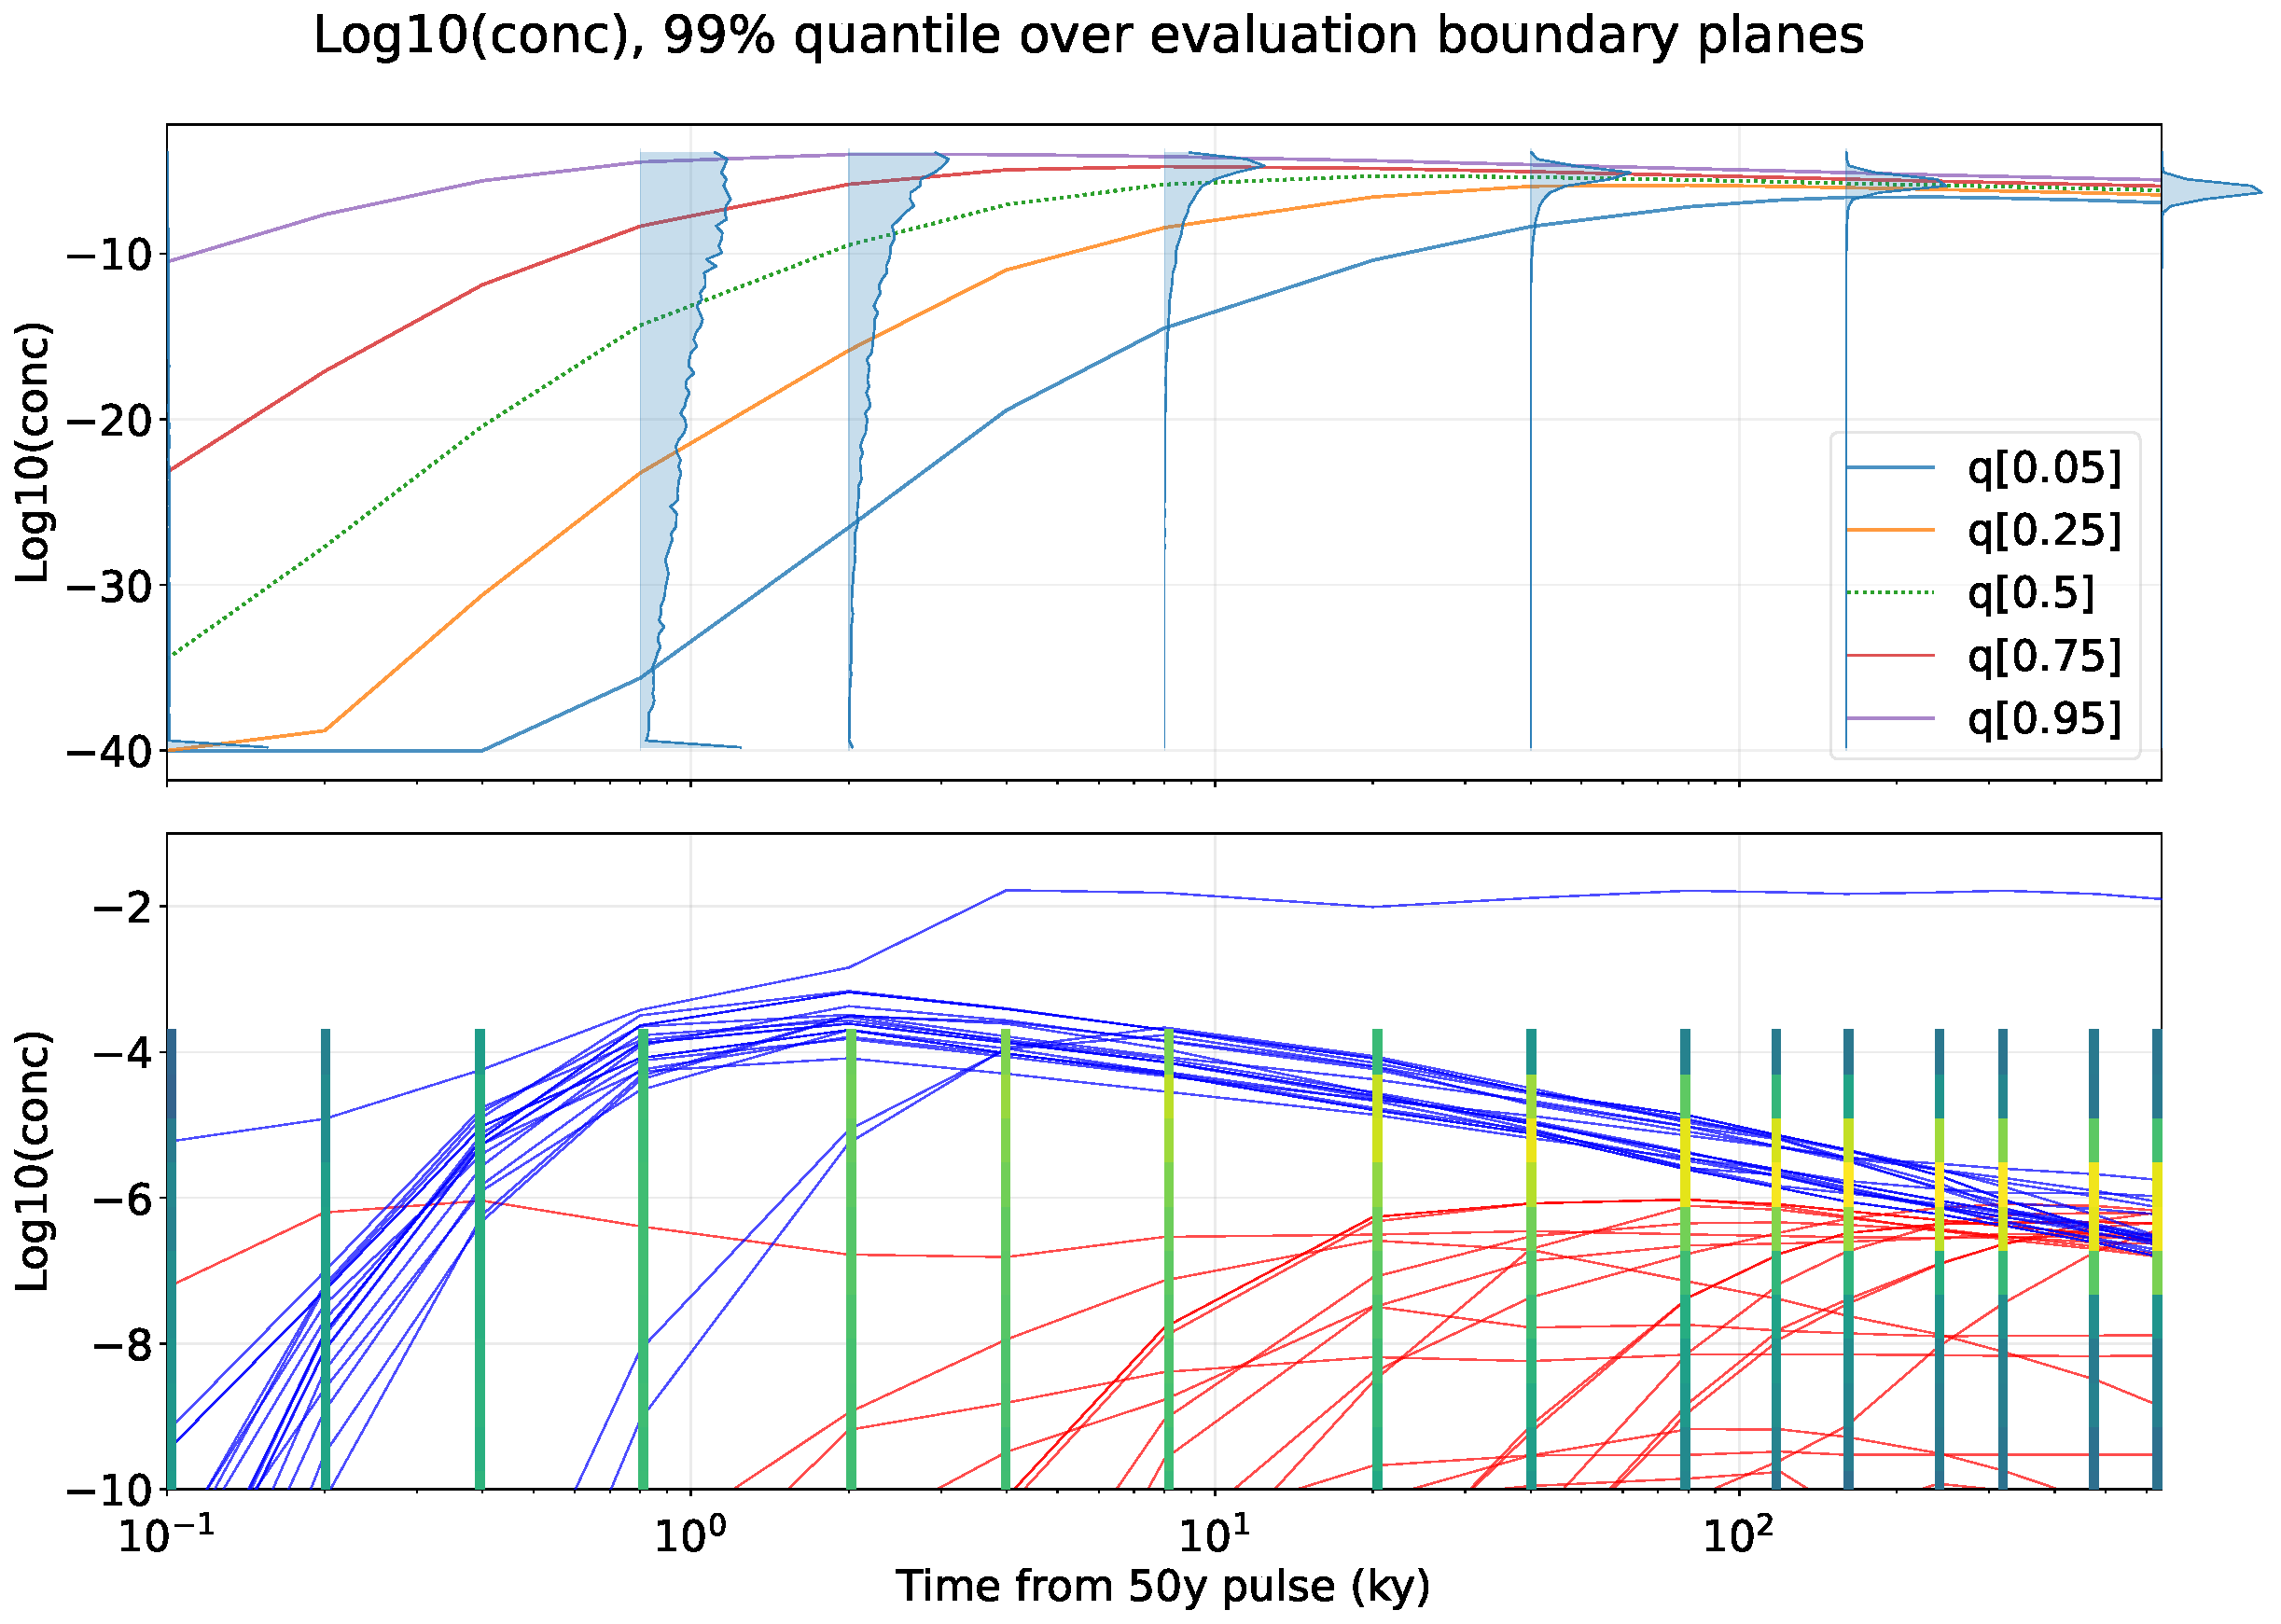
\includegraphics[width=0.9\textwidth]{graphics_tr/results/case_00a_hist_conc_over_time.pdf}
    % workdir_41d_test_ot_2048
    \caption{\textbf{Case 0}. Time-dependent density function of \gls{QoI} up to $\num{640e3}$ years. PDF and selected quantiles  (top), 20 smallest (red) and 20 largest (blue) samples, and a colormap representation of the density function.}
    \label{fig:case_00_conc}
\end{figure}
\begin{figure}[!htb]
    \centering
    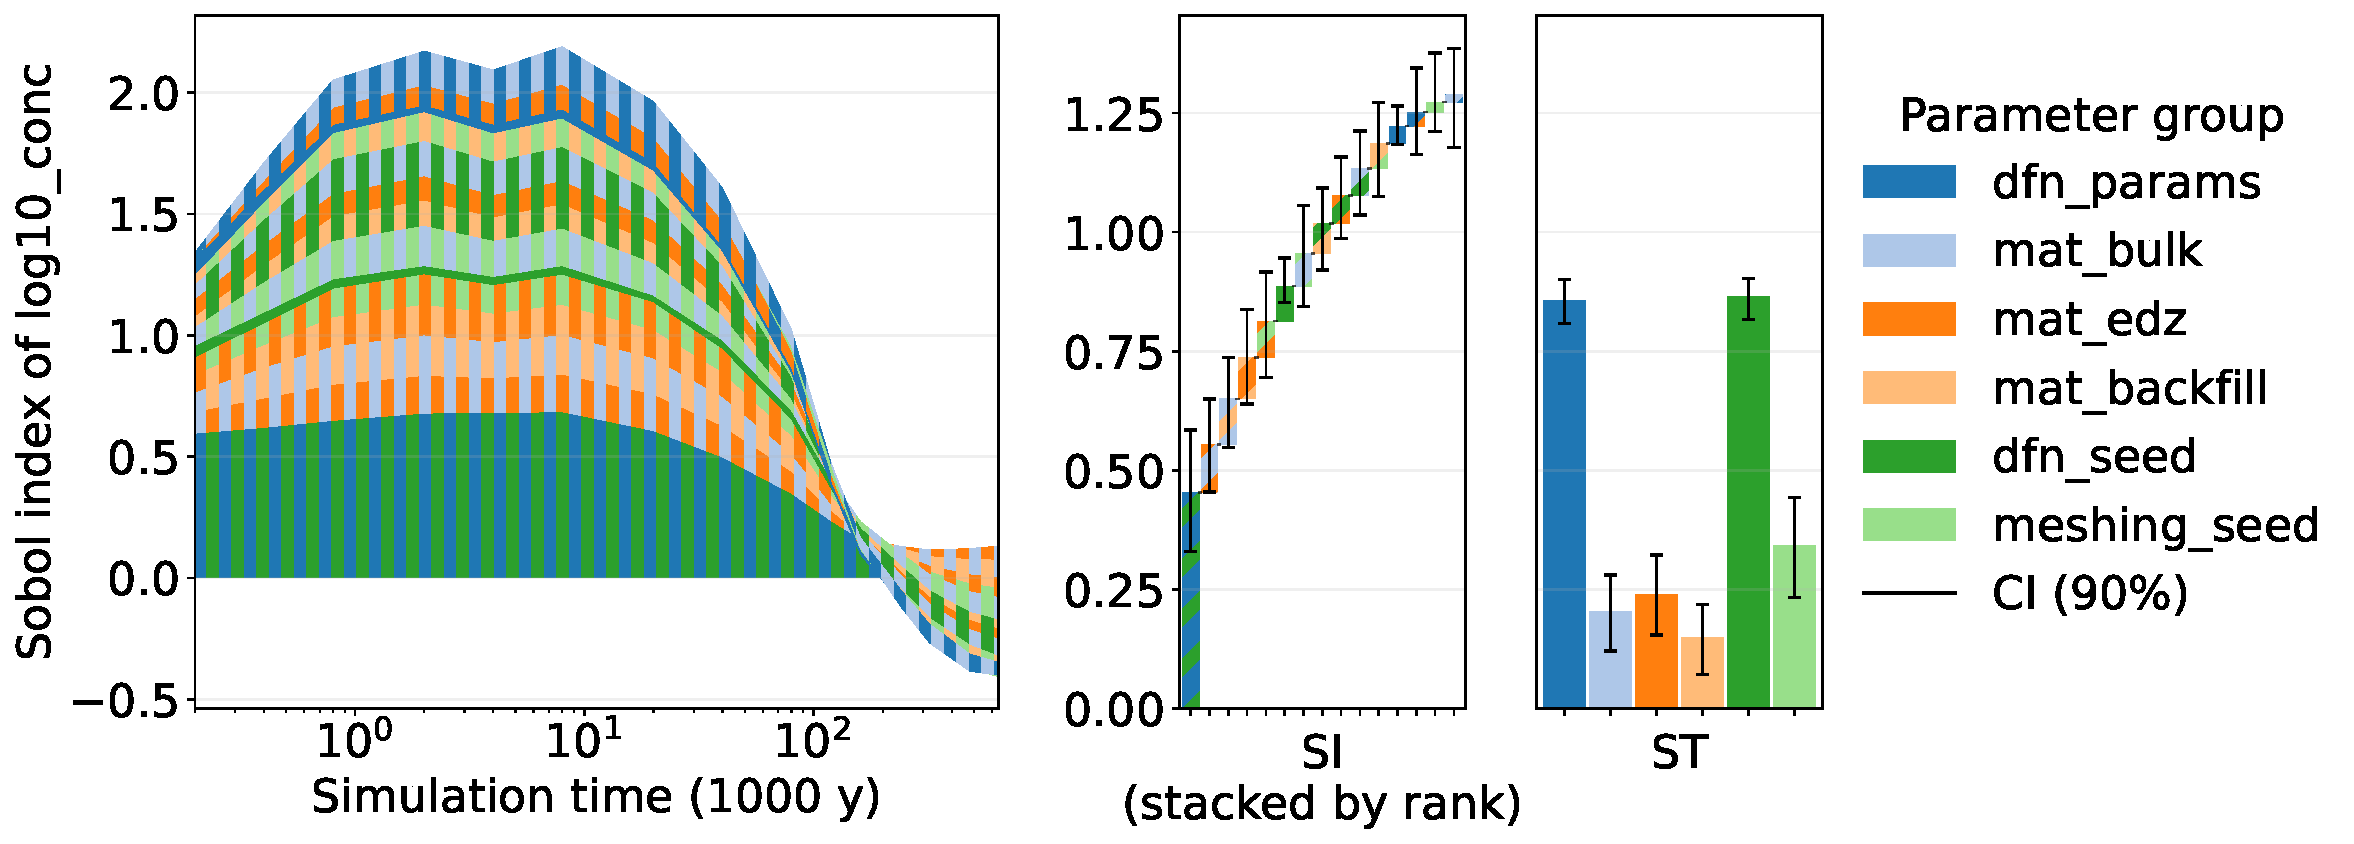
\includegraphics[width=0.9\textwidth]
    {graphics_tr/results/case_00a_sobol_agg_over_time.pdf}
    % workdir_41d_test_ot_2048
    \caption{\textbf{Case 0}. Sobol indices for $I(t)$ (left) and for $I=\max I(t)$ (right). Plain colors mark S1 indices, while stripes indicate S2 indices for pairs of parameter interactions. The S1 and S2 indices are stacked by rank, whereas the total-effect indices ST follow the parameter order. Error bars indicate estimated $90\%$ confidence intervals. Note that the estimated sums of Sobol indices may exceed the theoretical limit of 1 due to sampling error.
    }\label{fig:case_00_sobol}
\end{figure}
% \begin{figure}[!htb]
%     \centering
%     \includegraphics[width=0.9\textwidth]
%     {graphics_tr/results/case_00_sobol_agg_table.pdf}
%     % workdir_41d_test_ot_2048
%     \caption{\pe{\textbf{Case 1}. Table of Sobol indices.}}\label{fig:var_01_sobol_table}
% \end{figure}



%%%%% Case 01
%%%%%%%%%%%%%%%%%%%%%%%%%%%%%%%%%%%%%%%%%%%%%%%%%%%%%%%%%%%%
\FloatBarrier
\subsubsection{Case 1}
In this case, the DFN is omitted and transport proceeds only through the rock matrix and the backfill, providing the most conservative scenario. As shown in \figref{fig:case_1_conc}, the \gls{QoI} increases only slowly. The breakthrough time is approximately $100\,\munit{ky}$ and its variability is small compared with the DFN cases. Consistent with the slower contaminant migration, the variance of the \gls{QoI} also decreases more slowly over time.

The sensitivity analysis includes the following parameter groups:
\begin{enumerate}
    \item bulk rock: $k_r$, $\theta_r$, $d_r$, $\alpha_{Lr}$
    \item backfill: $k_b$, $\theta_b$, $d_b$, $\alpha_{Lb}$
    \item EDZ: $\tilde k_e$, $\tilde \theta_e$, $\tilde w_e$
    \item meshing seed
\end{enumerate}

The first-order Sobol indices (S1) are close to the corresponding total-effect indices (ST), indicating weak interaction effects, see \figref{fig:case_1_sobol}. The dominant contributions to output variability come from the bulk-rock and EDZ parameter groups, while the influence of the backfill parameters declines in time and its total effect is least significant. The contribution of numerical uncertainty due to meshing, as well as the remaining variance attributable to interactions, is negligible.


\begin{figure}[!htb]
    \centering
    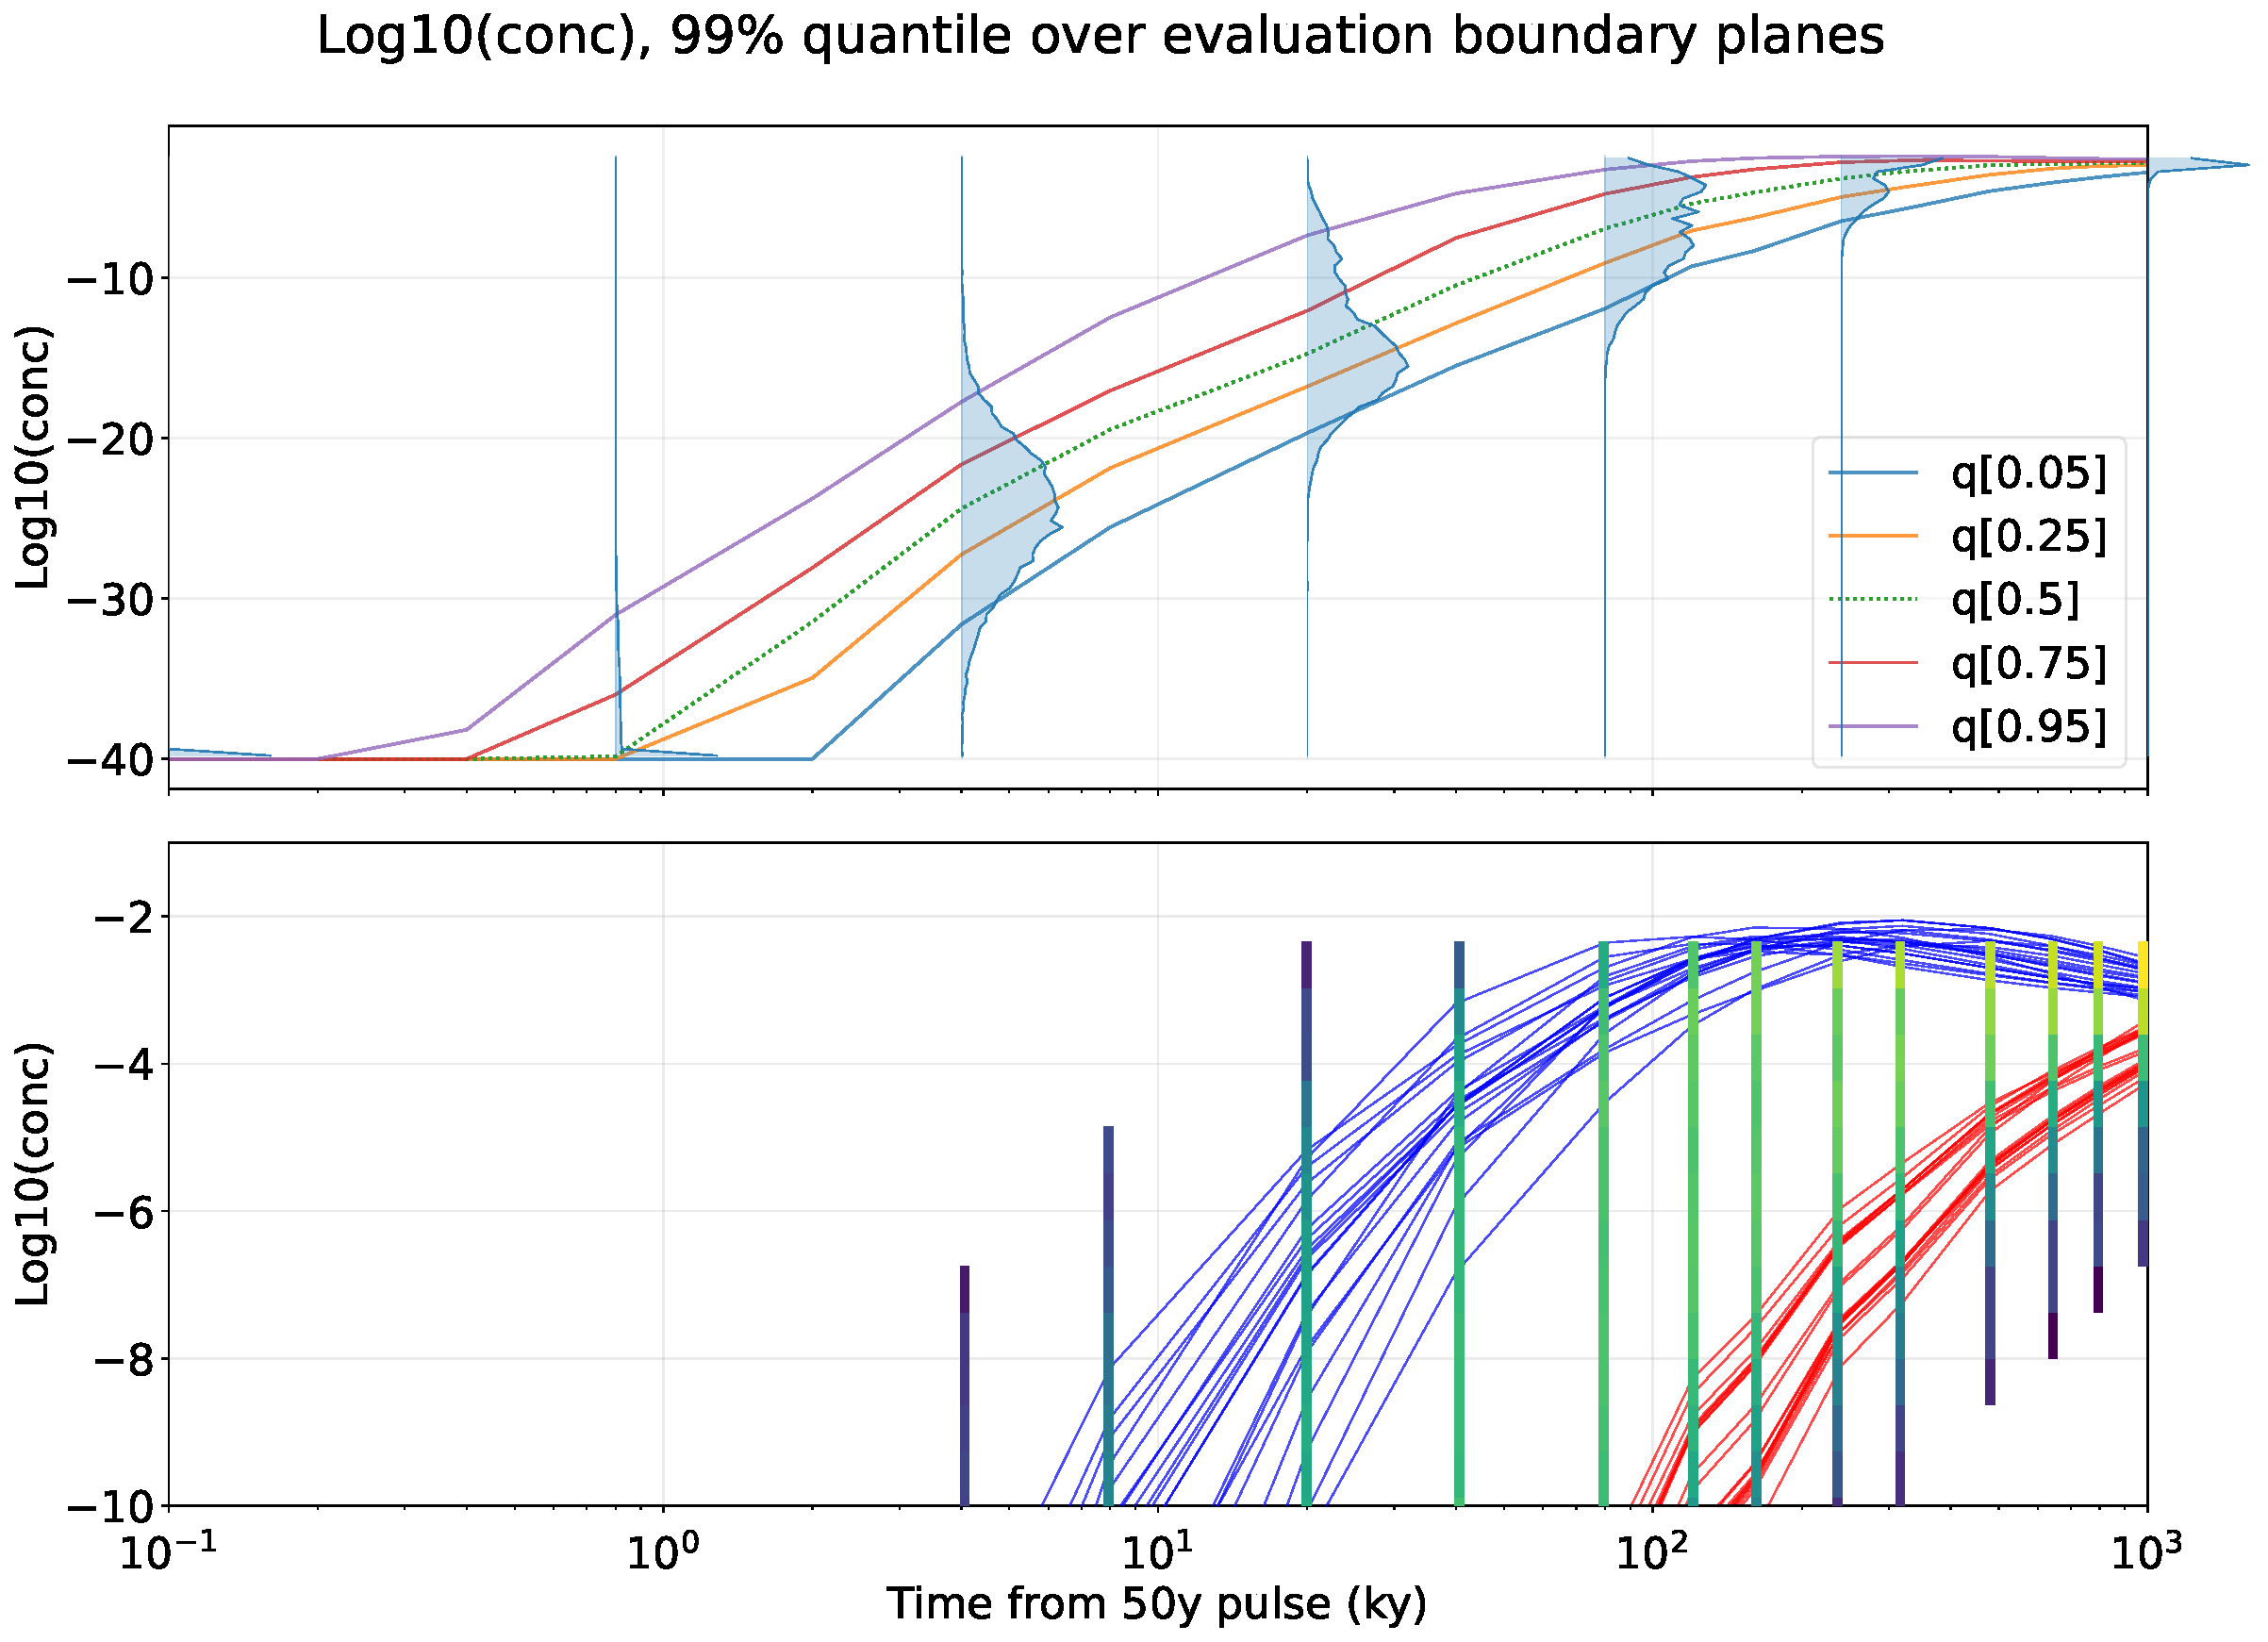
\includegraphics[width=0.9\textwidth]{graphics_tr/results/case_1a_hist_conc_over_time.pdf}
    % workdir_40b_test_ot_2048
    \caption{\textbf{Case 1}. Concentration indicator value over time up to $10^6$ years.}\label{fig:case_1_conc}
\end{figure}
\begin{figure}[!htb]
    \centering
    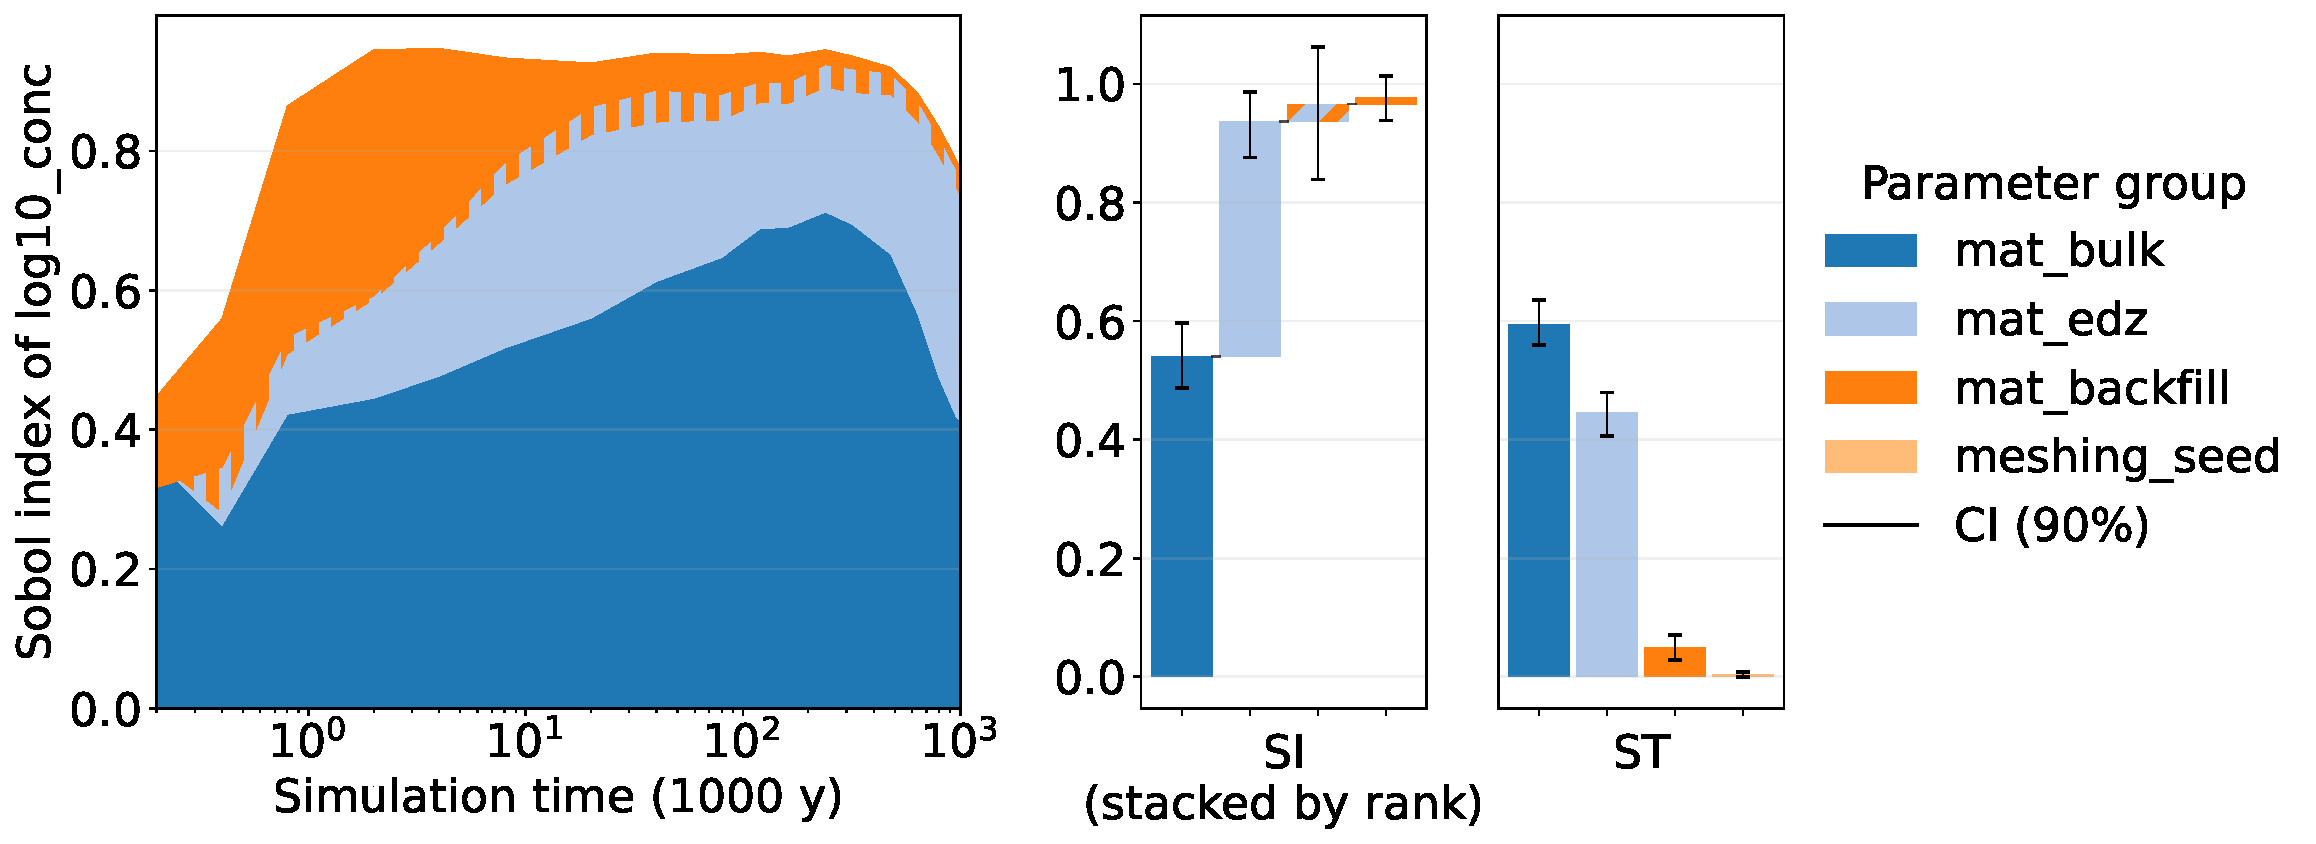
\includegraphics[width=0.9\textwidth]
    {graphics_tr/results/case_1a_sobol_agg_over_time.pdf}
    % workdir_40b_test_ot_2048
    \caption{\textbf{Case 1}. Sobol indices for $I(t)$ (left) and for $I=max I(t)$ (right).}\label{fig:case_1_sobol}
\end{figure}
% \begin{figure}[!htb]
%      \centering
%      \includegraphics[width=0.9\textwidth]
%      {graphics_tr/results/case_1a_sobol_agg_table.pdf}
%      % workdir_40b_test_ot_2048
%      \caption{\textbf{Case 1}. Table of Sobol indices.}\label{fig:var_00_sobol_table}
% \end{figure}


%%%%%% Case 02b
%%%%%%%%%%%%%%%%%%%%%%%%%%%%%%%%%%%%%%%%%%%%%%%%%%%%%%%%%%%%
\FloatBarrier
\subsubsection{Case 2}
We consider a variant of \emph{Case 0} with a refined treatment of DFN uncertainty. The DFN parameters are split into (i) geometric descriptors of the network (\emph{DFN population}) and (ii) fracture transmissivity parameters (\emph{DFN transport}). To reduce computational costs, the bulk-rock and backfill parameters are merged into a single group denoted \emph{material parameters}.

The sensitivity analysis includes the following parameter groups:
\begin{enumerate}
    \item material parameters (\verb|mat_BB|): $k_r$, $\theta_r$, $d_r$, $\alpha_{Lr}$, $k_b$, $\theta_b$, $d_b$, $\alpha_{Lb}$
    \item EDZ: $\tilde k_e$, $\tilde \theta_e$, $\tilde w_e$
    \item DFN population: $(p_{30}, \alpha)^{(i)}$
    \item DFN transport: $a^{(i)}$
    \item DFN realization (seed)
    \item meshing seed
\end{enumerate}

The time evolution in \figref{fig:case_02_conc} closely follows Case~0. Figure~\ref{fig:case_02_sobol} is also qualitatively similar, but with several clear differences.
The estimated total-effect indices remain close to those of Case~0; however, the separated group of fracture-transport parameters now contributes about $5~\%$ of the output variability.
The output variance is again driven primarily by interaction effects between the DFN population parameters and the particular DFN realization.
The contribution of numerical uncertainty due to meshing is more pronounced, and the interaction between the DFN realization seed and the meshing seed is significant.
Within the DFN parameterization, the geometric group (\emph{DFN population}) dominates, whereas the transmissivity group (\emph{DFN transport}) contributes only a small share of the variance. However, the former group is based on Bayesian inversion with a comparatively well-characterized uncertainty representation, while the latter uses a rough estimate derived from Forsmark site case studies, so its uncertainty may be underestimated.


\begin{figure}[!htb]
    \centering
    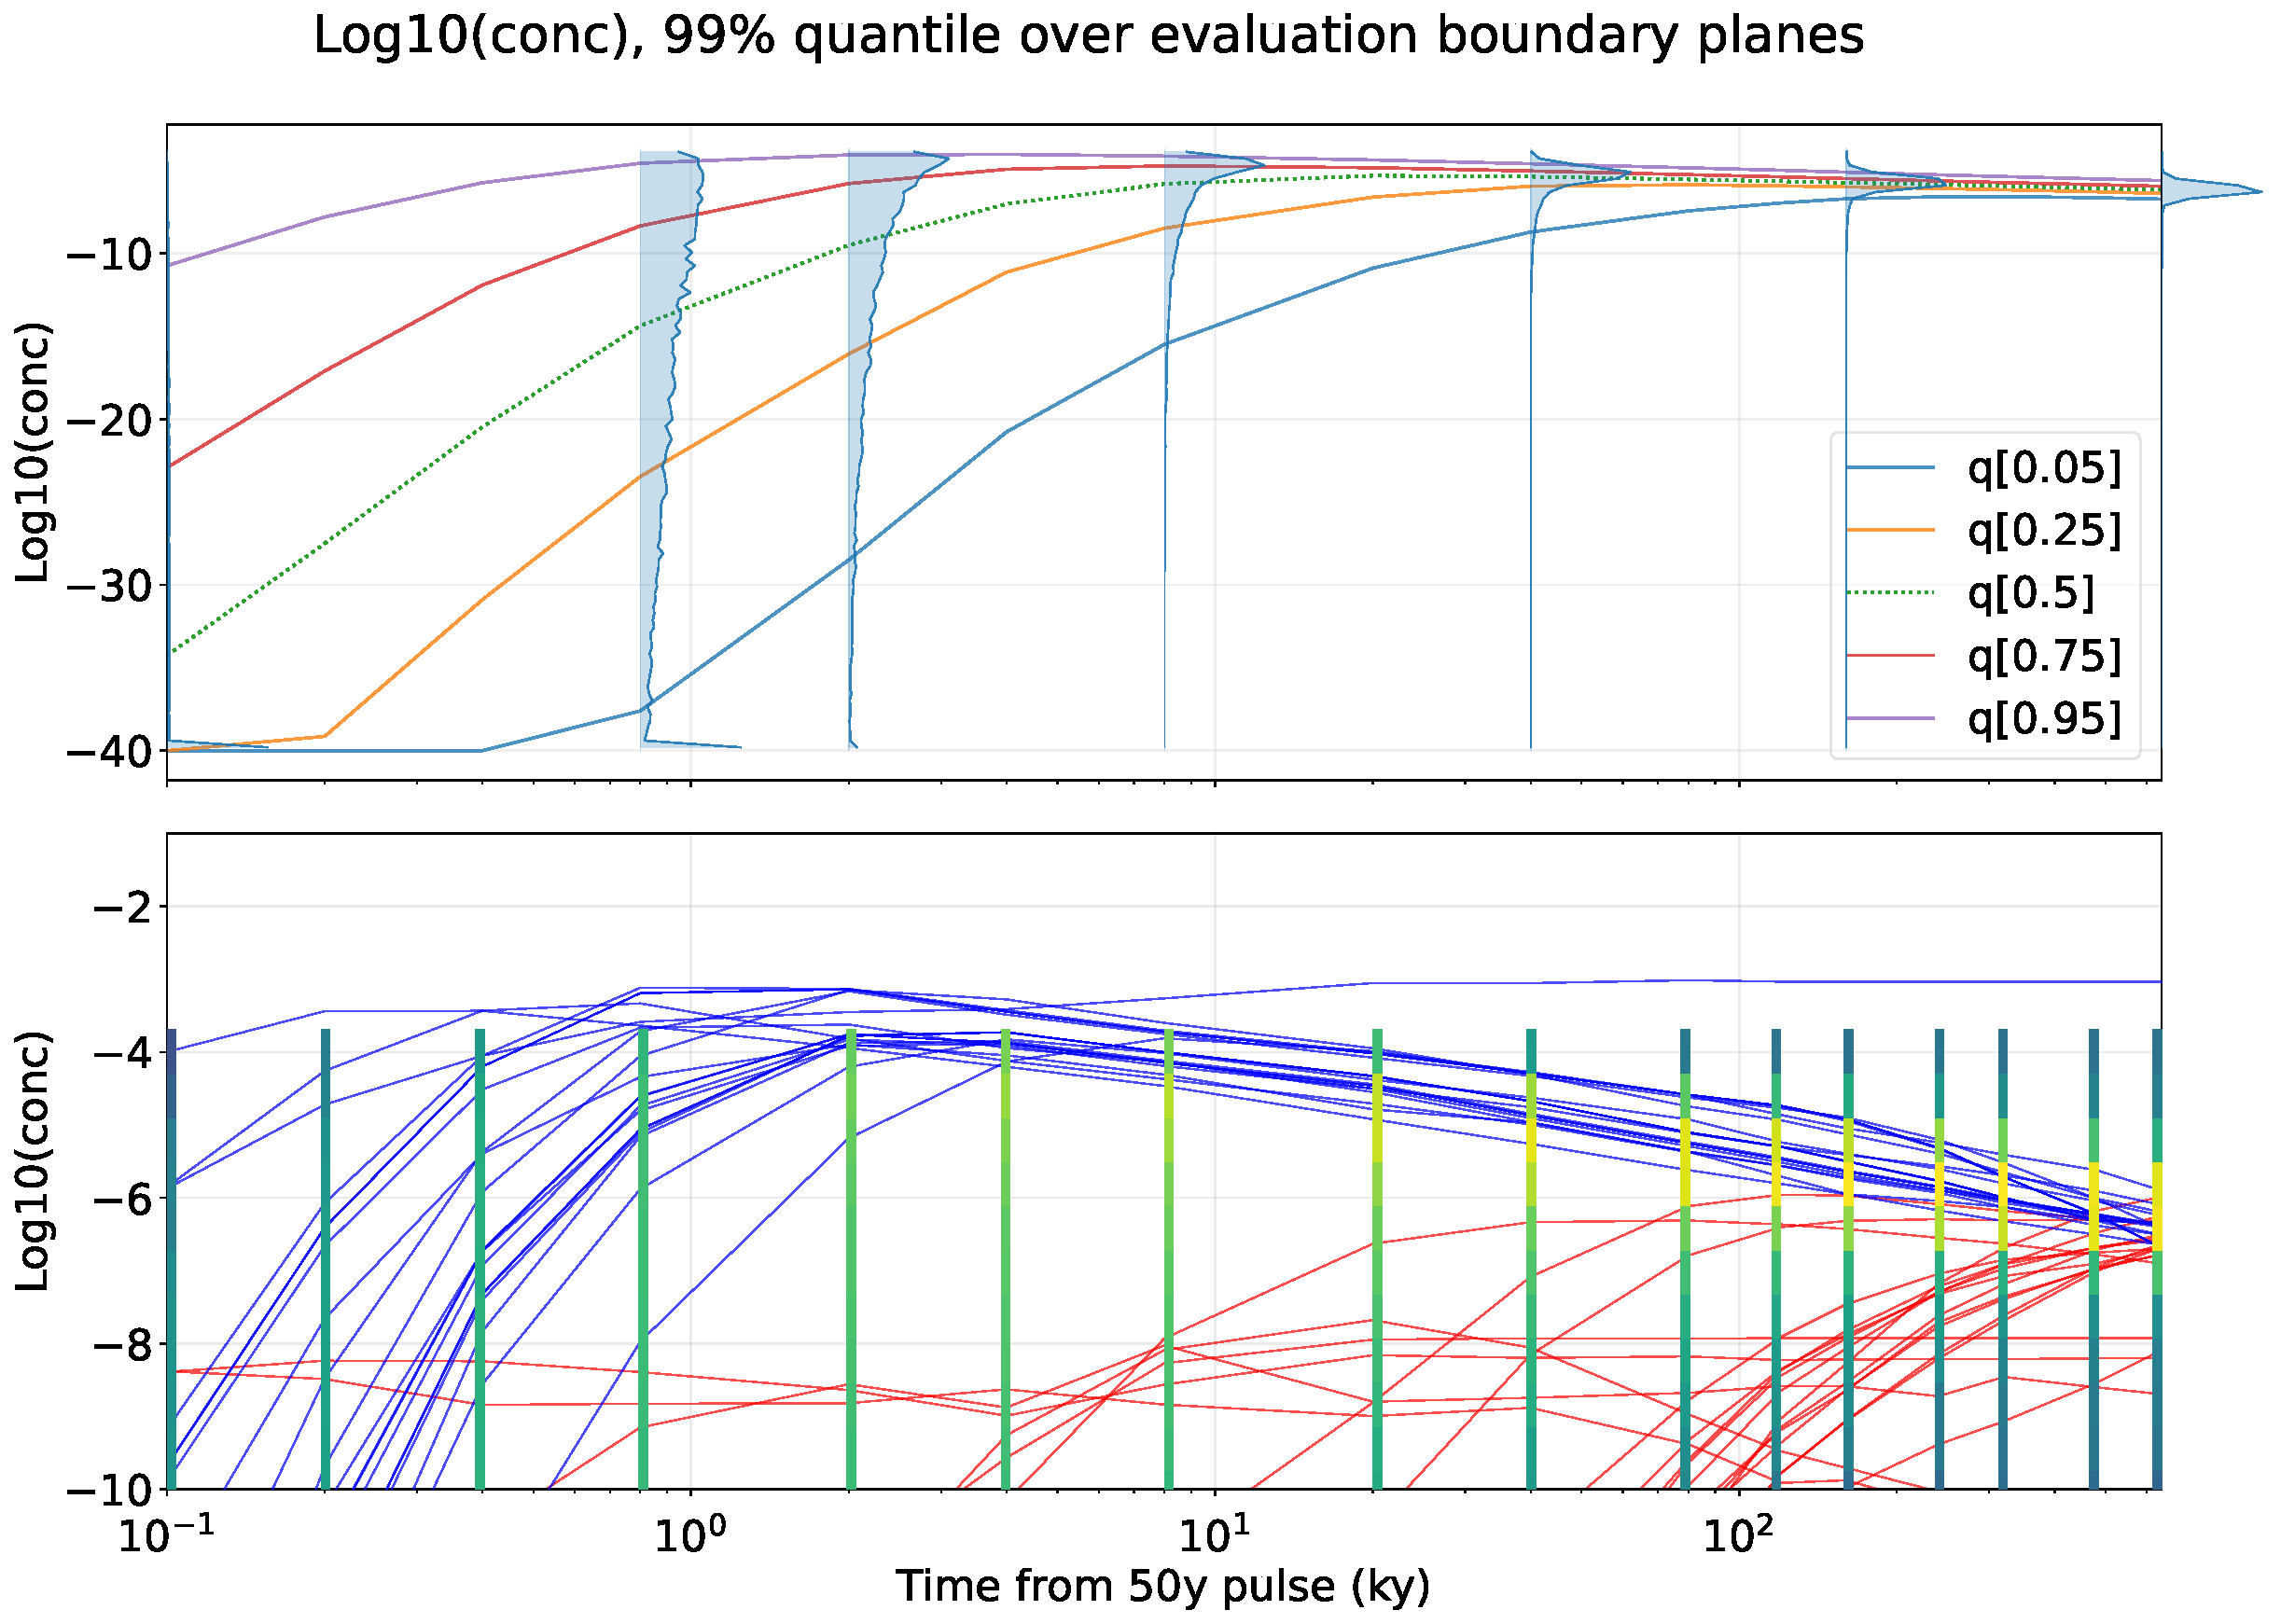
\includegraphics[width=0.9\textwidth]{graphics_tr/results/case_02_hist_conc_over_time.pdf}
    % workdir_42c_test_ot_2048
    \caption{\textbf{Case 2}. Concentration indicator value over time up to $10^6$ years.}\label{fig:case_02_conc}
\end{figure}
\begin{figure}[!htb]
    \centering
    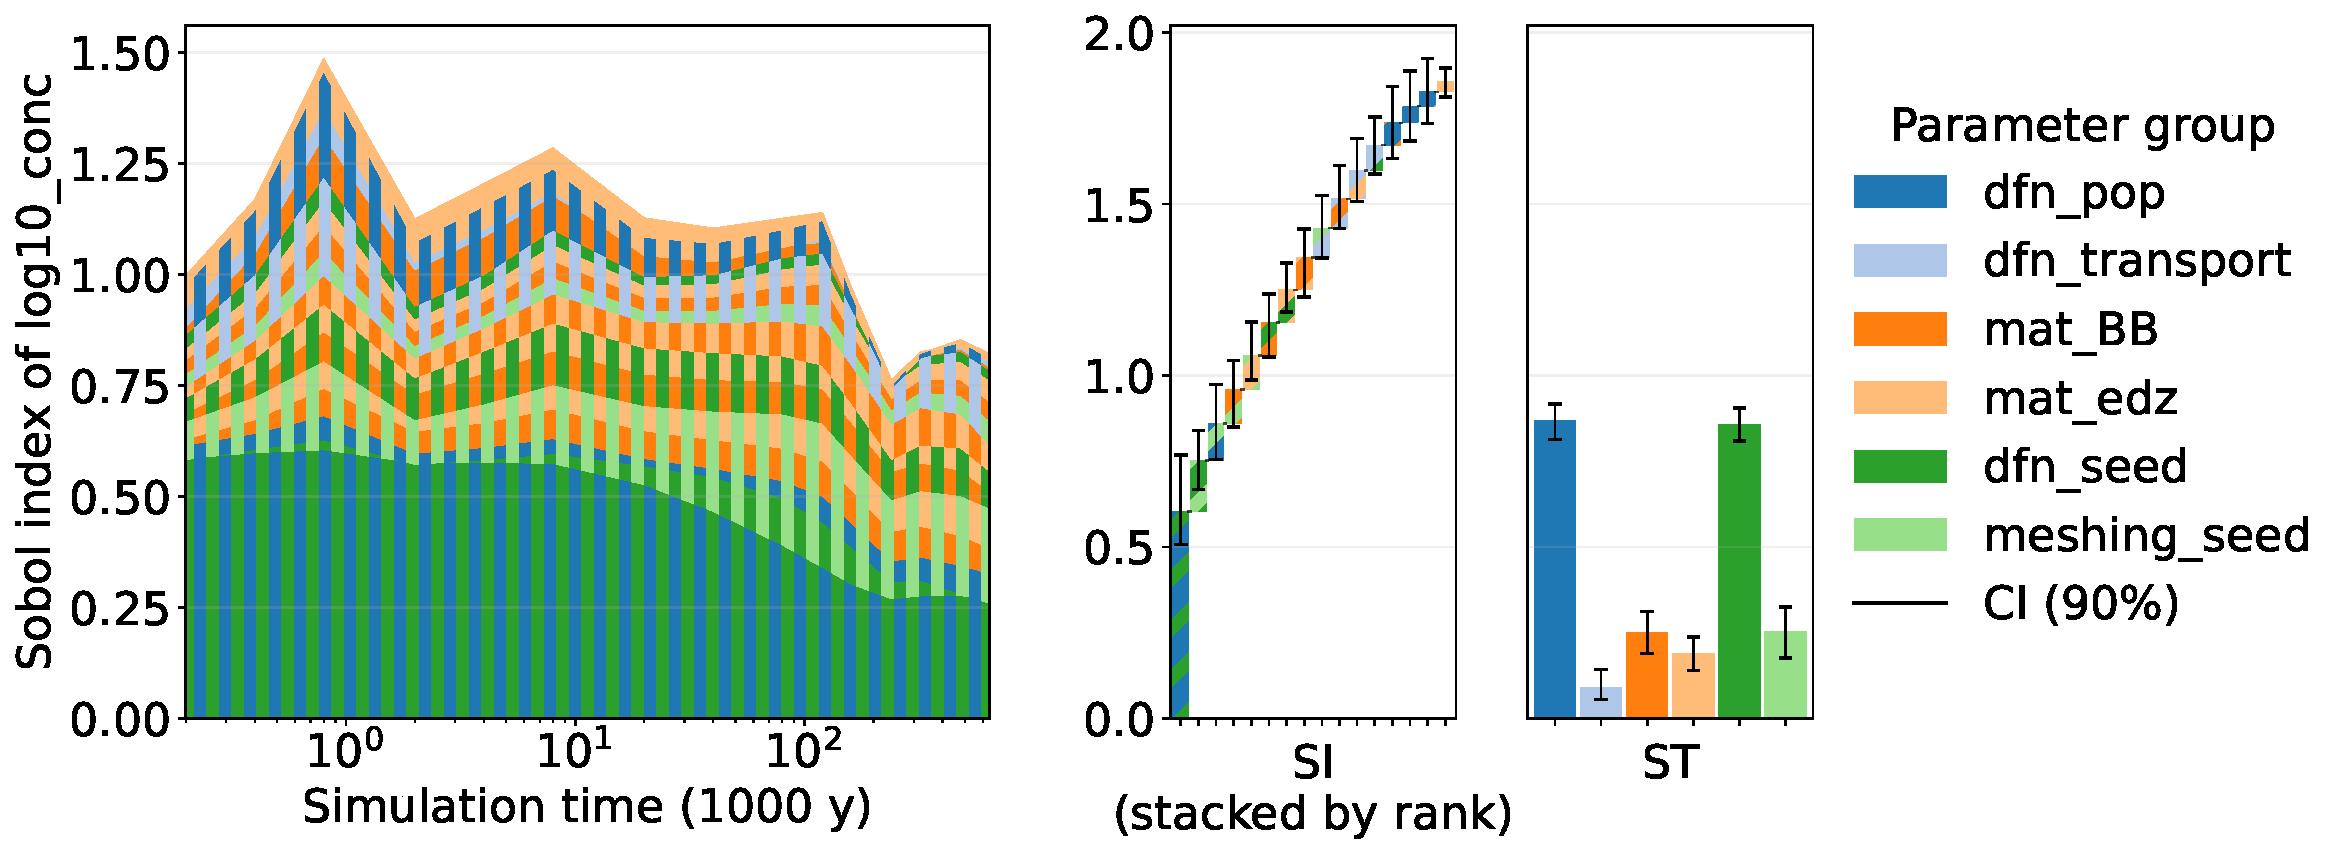
\includegraphics[width=0.9\textwidth]
    {graphics_tr/results/case_02_sobol_agg_over_time.pdf}
    % workdir_42c_test_ot_2048
    \caption{\textbf{Case 2}. Sobol indices for $I(t)$ (left) and for $I=max I(t)$ (right).}\label{fig:case_02_sobol}
\end{figure}
% \begin{figure}[!htb]
%     \centering
%     \includegraphics[width=0.9\textwidth]
%     {graphics_tr/results/var_02b_sobol_agg_table.pdf}
%     % workdir_42c_test_ot_2048
%     \caption{\pe{\textbf{Case 2}. Table of Sobol indices.}}\label{fig:case_02_sobol_table}
% \end{figure}


% {\bf Discussion}
% The estimated Sobol indices suggests strong sensitivity to the interaction between DFN parameters and particular network sample, however the first order (S1) indices are small.
    
% \begin{itemize}

%     \item The estimation error of the interaction Sobol indices is high however and even the provided confidence intervals are
%     rather qualitative. Need a sample size at least $N=4000$ (doable)
%     or even $N=16000$ to get any relevant information about other interactions.
%     \item The numerical uncertainty is indicated by uncertainty due to computational mesh, but could be higher if we account for the effect of time discretization. It is small compared to the main interaction, but still at least comparable to the other uncertainties.  In order to reduce  this error, we should 
%     apply subsampling over different meshes and use average to
%     stabilize the model output. The similar technique could be used to artificially remove effect of other uncertainties to obtain 
%     comparison of the parameters of smaller effect.
% \end{itemize}

%%%%%% Case 3
%%%%%%%%%%%%%%%%%%%%%%%%%%%%%%%%%%%%%%%%%%%%%%%%%%%%%%%%%%%%
\FloatBarrier
\subsubsection{Case 3}

A major limitation of the used transport model is the absence of an explicit representation of small-scale fractures in the size range $0.1$--$1\,\munit{m}$. 
Our \gls{DFM} approach is based on numerical homogenization of these fractures and their representation through an anisotropic, heterogeneous conductivity field using a convolutional neural network (\cite{Spetlik_Convolutional_2026}). However, the integration of the homogenization surrogate models is not yet available for problems involving complex internal geometry or material structure. 

The hydraulic conductivities used in Case~0 could be underestimated due to the missing small-scale fractures. For this reason, the present case (derived from Case~0) assumes elevated hydraulic conductivity, with $GM(k_r)=\num{1e-11}$ and $CIF(k_r)=100$. This range covers values from $\num{1e-13}$ measured on laboratory samples up to $\num{1e-9}$ observed in situ during \gls{WPT}s. Accordingly, the dispersivity, which depends on the variance of hydraulic conductivity, was adjusted to $GM(\alpha_L)=3$ and $CIF(\alpha_L)=3$.


The results are shown in \figref{fig:case_03_conc} and \figref{fig:case_03_sobol}. In contrast to Case~0, the breakthrough times are shorter, allowing the simulations to cover the early phase of the concentration decline. The concentration variability is also substantially higher.
As expected, the influence of DFN-related parameters, including the DFN realization and numerical uncertainty, remains significant. However, the reduction in the Sobol indices of the remaining material-parameter groups is somewhat counterintuitive, and among them only the bulk-rock material group remains clearly significant.

A plausible explanation is that once the background rock conductivity and dispersivity are increased, transport becomes less controlled by contrasts among the engineered-barrier domains and more controlled by the connectivity of the surrounding rock and the realized fracture geometry. In that regime, the backfill and EDZ parameters mainly perturb already efficient pathways, whereas the bulk-rock parameters still affect the overall residence time in the matrix and the strength of matrix-bridge transport between fractures. 


\begin{figure}[!htb]
    \centering
    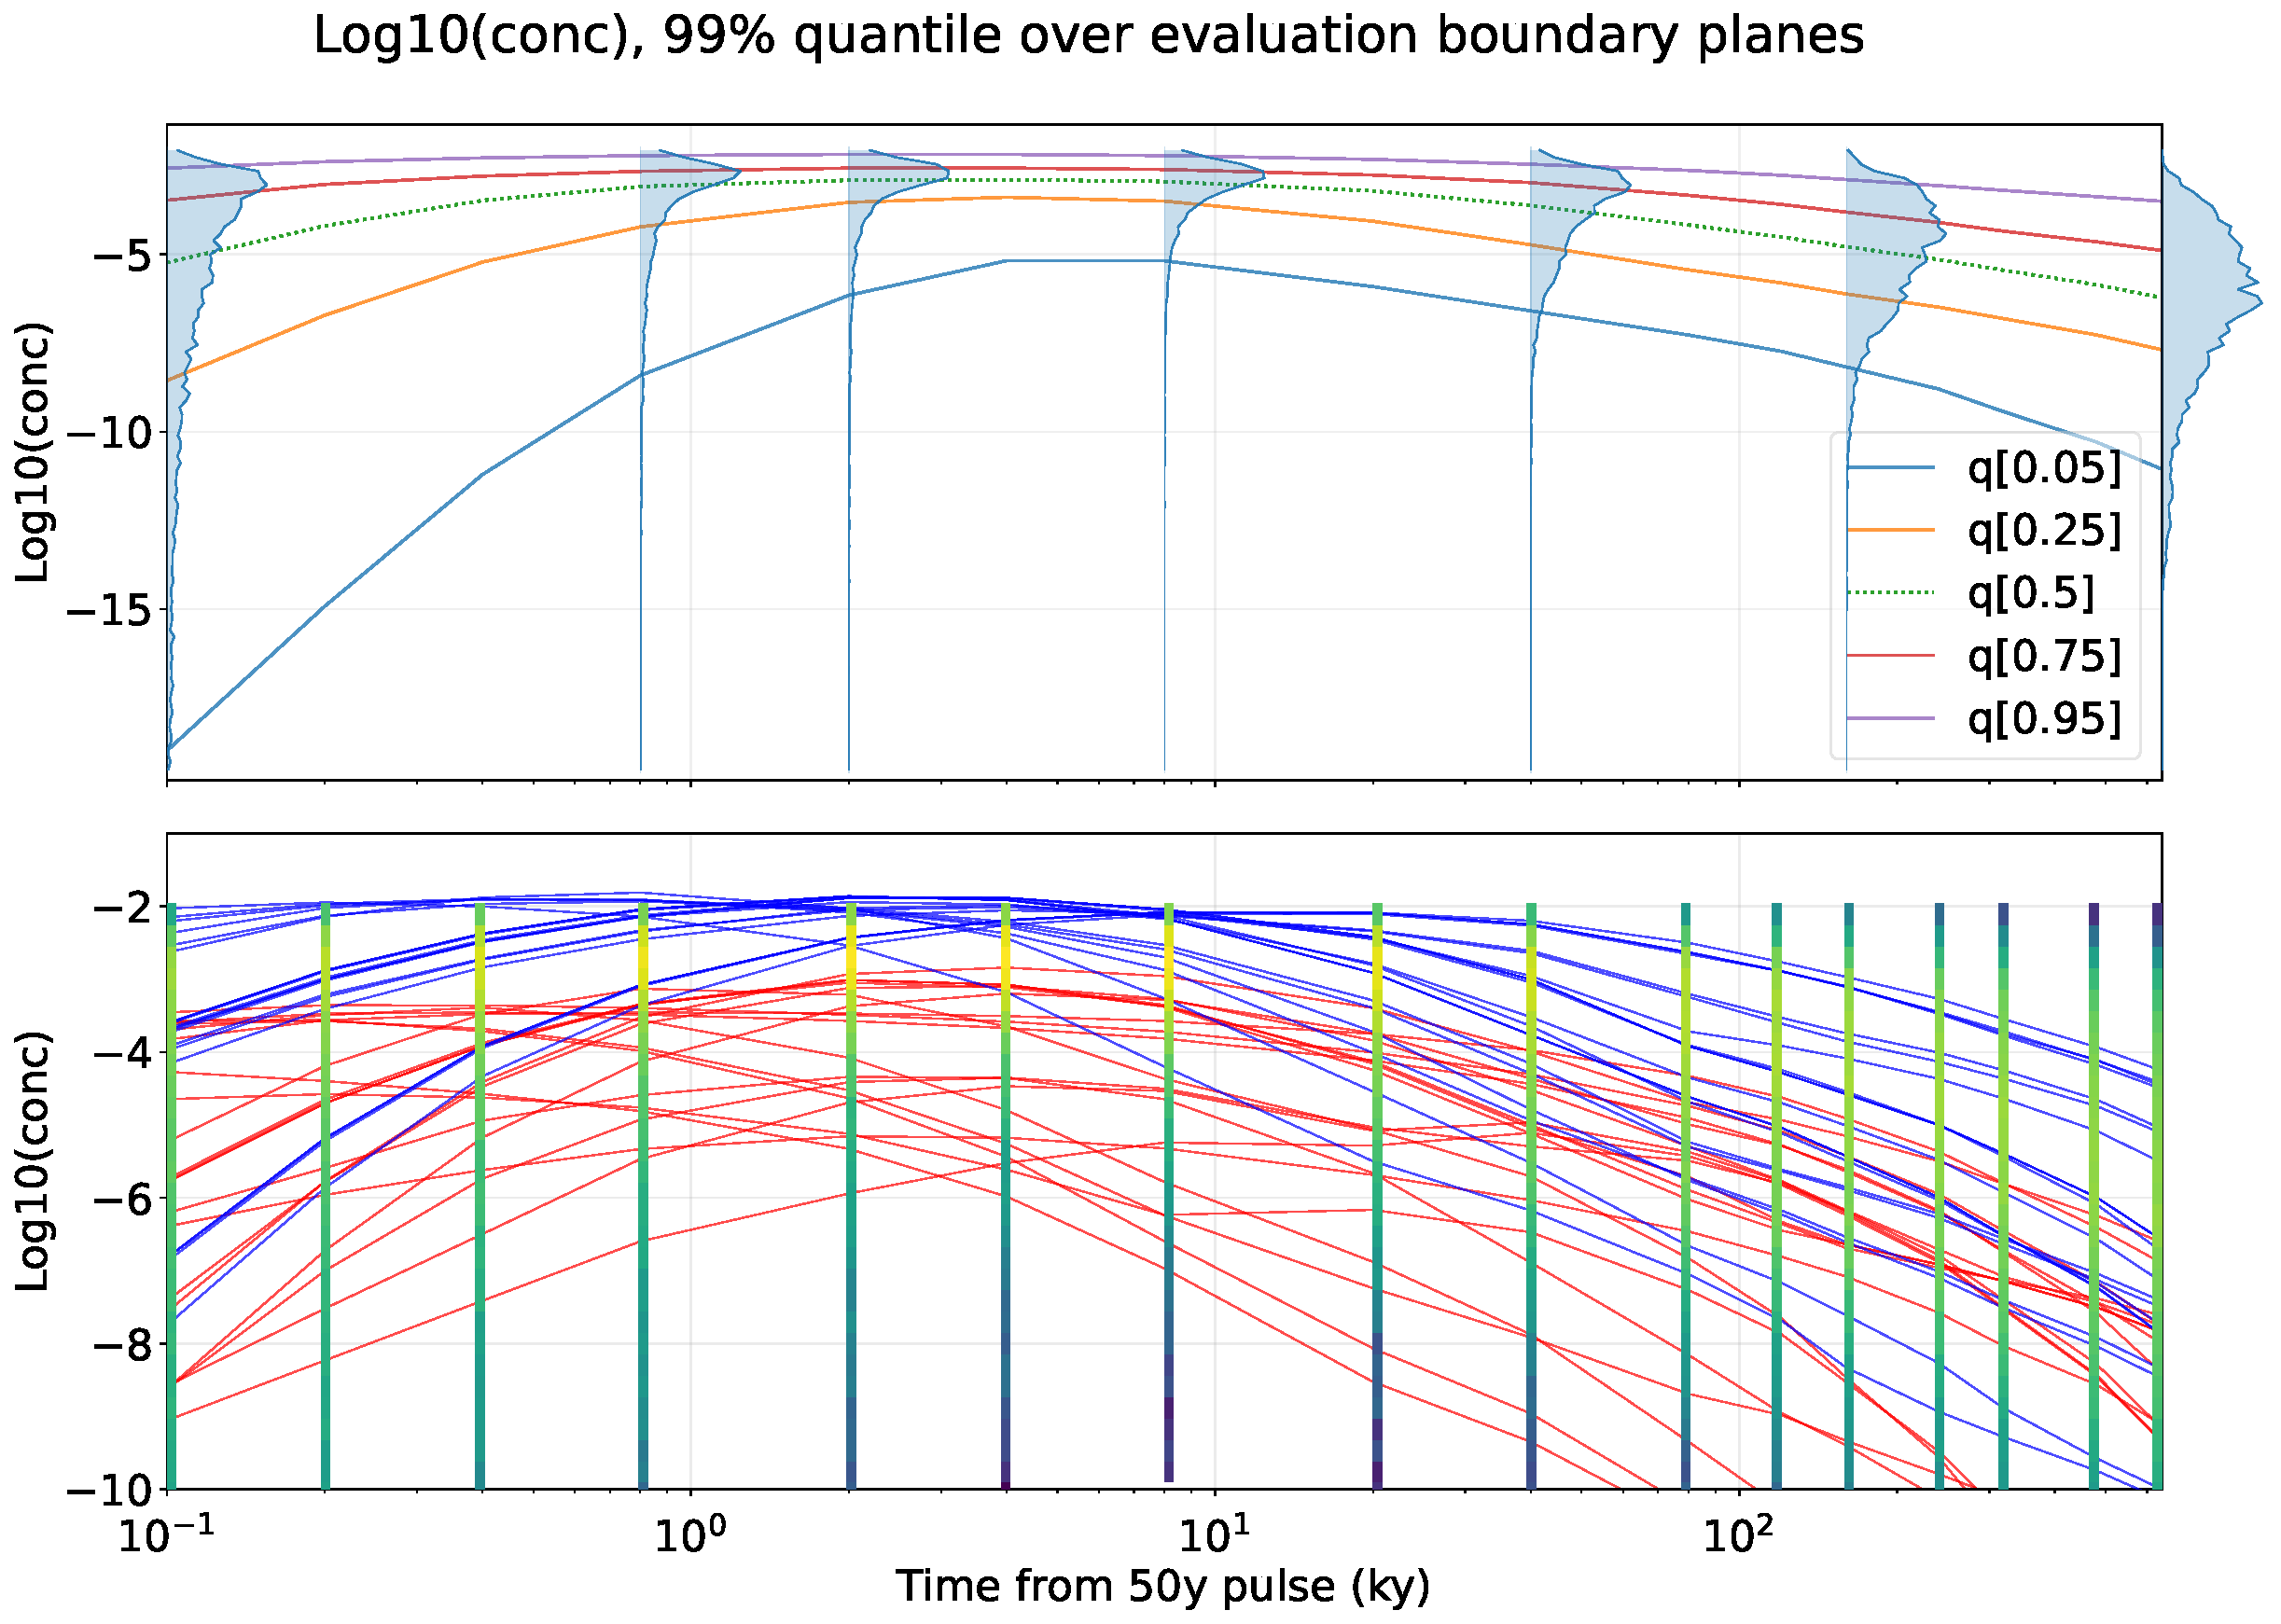
\includegraphics[width=0.9\textwidth]{graphics_tr/results/case_00b_hist_conc_over_time.pdf}
    % workdir_43c_test_ot_2048
    \caption{\textbf{Case 3}. Concentration indicator value over time up to $10^6$ years.}\label{fig:case_03_conc}
\end{figure}
\begin{figure}[!htb]
    \centering
    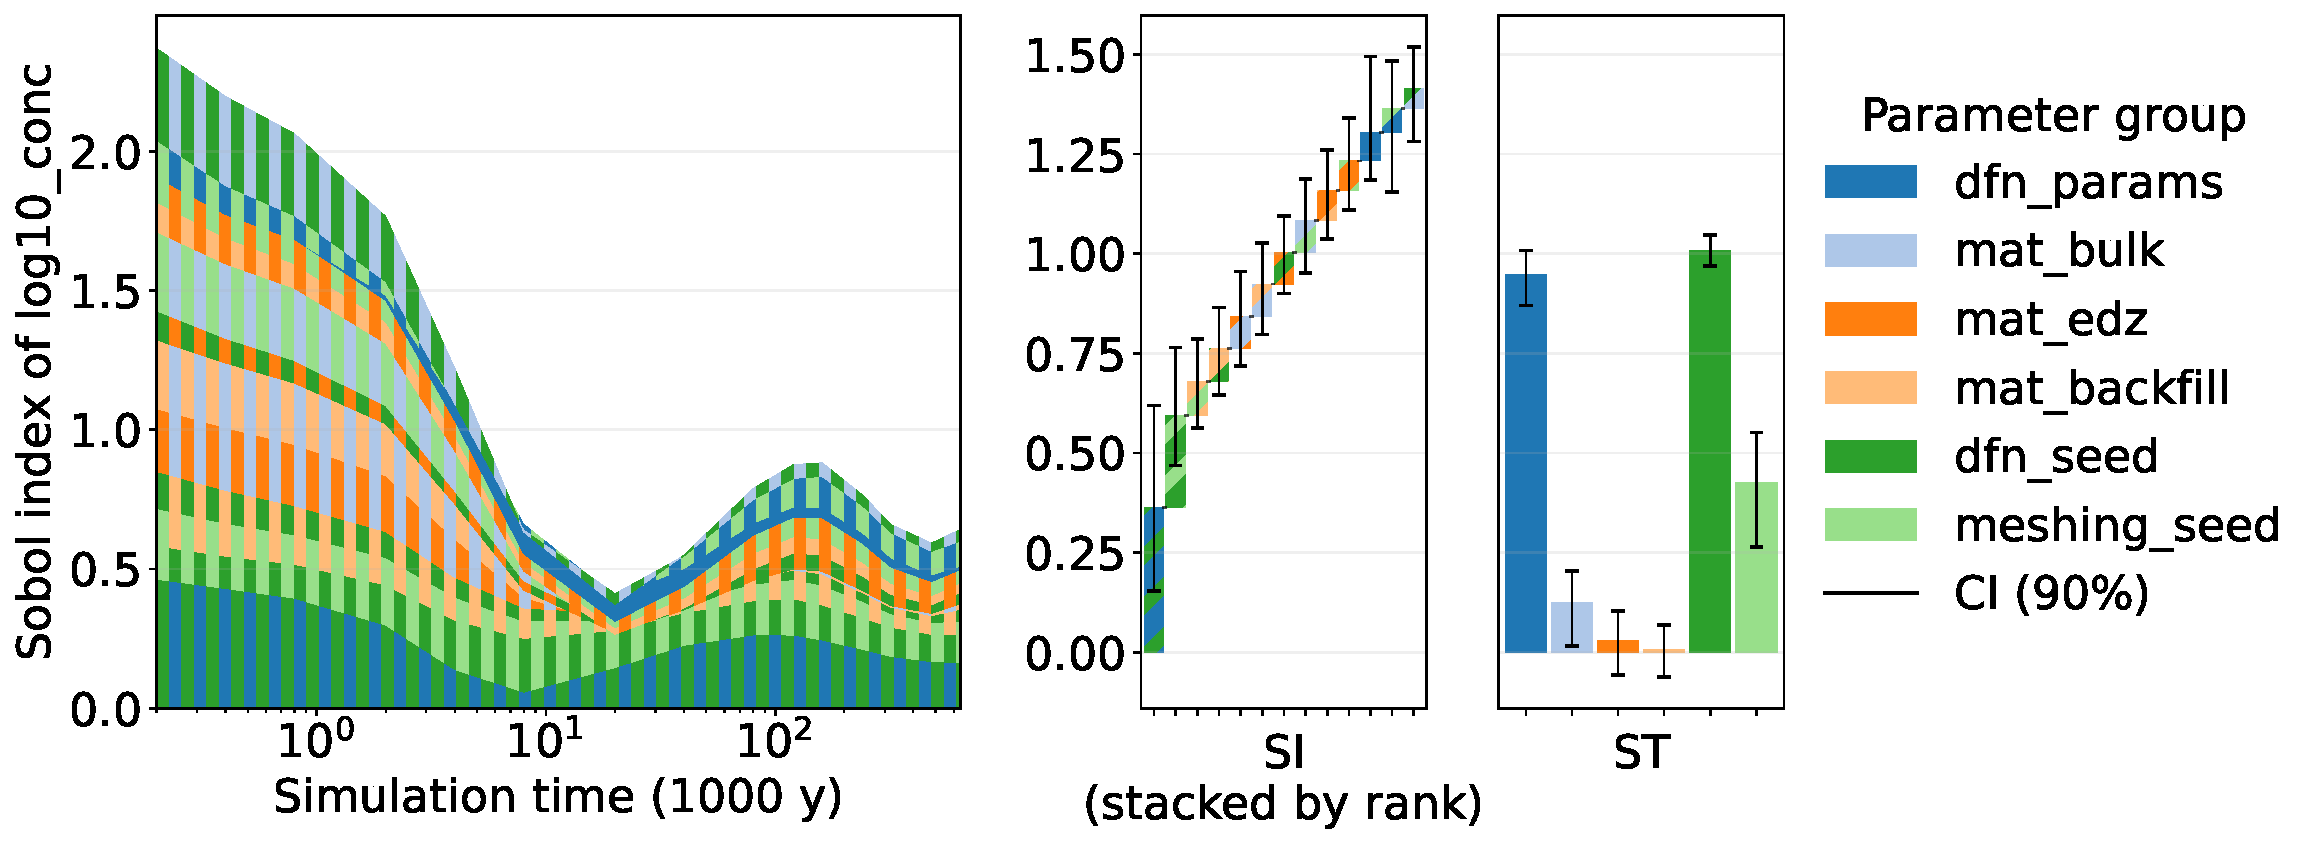
\includegraphics[width=0.9\textwidth]
    {graphics_tr/results/case_00b_sobol_agg_over_time.pdf}
    % workdir_43c_test_ot_2048
    \caption{\textbf{Case 3}. Sobol indices for $I(t)$ (left) and for $I=max I(t)$ (right).}\label{fig:case_03_sobol}
\end{figure}
% \begin{figure}[!htb]
%     \centering
%     \includegraphics[width=0.9\textwidth]
%     {graphics_tr/results/case_00b_sobol_agg_table.pdf}
%     % workdir_43c_test_ot_2048
%     \caption{\pe{\textbf{Case 3}. Table of Sobol indices.}}\label{fig:case_03_sobol_table}
% \end{figure}



\FloatBarrier
\section{Chapter summary}
\label{sec:tr_conclusions}


We have constructed a near-field transport model for a single leaking \gls{WDP} in an access-tunnel segment, explicitly resolving the bentonite/backfill and EDZ domains. Flow and transport in the surrounding rock are represented by a mixed-dimensional \gls{DFM} formulation with a stochastically generated \gls{DFN}. A complementary hydro-mechanical analysis was used to estimate permeability changes induced  by excavation and \gls{DGR} closure. It was used to define uncertainty ranges for EDZ parameters. These model components were combined with a stochastic description of key inputs, enabling a variance-based sensitivity analysis using Sobol indices for parameter groups.

The transport model is diffusion-dominated for the considered parameter ranges. Locally, advection can become more pronounced along major fractures and along short ``matrix bridges'' connecting fractures, but sustained advection-dominated behaviour is unlikely even under substantially higher velocities because increasing velocities also increase hydrodynamic dispersion.



The DFN has a decisive effect on breakthrough. In the nominal fractured scenario (Case~0), the characteristic breakthrough time is on the order of $2\,\munit{ky}$, but with very large variability, ranging from about $0.11\,\munit{ky}$ to several $100\,\munit{ky}$. In contrast, the DFN-free control case (Case~1) delays breakthrough to roughly $100\,\munit{ky}$ and exhibits much smaller variability. Consistent with progressive mixing and the diminishing influence of early-time pathways, the variance of the time-dependent \gls{QoI} $I(t)$ decreases with time; we therefore also interpret results using the aggregated scalar quantity $\max I(t)$, which captures the peak concentration over the full simulation horizon.

The sensitivity analysis shows that, once fractures are present, the dominant contributions to the output variance come from the realized fracture geometry and the DFN parameterization. In Case~0, the DFN realization and DFN parameter group dominate the total-effect indices, while first-order effects remain small and the main influence arises through interactions. The strongest and most robust interaction is between the DFN realization and the DFN parameter group, implying that variance reduction requires improving DFN characterization; however, simply fitting DFN parameters to larger outcrop datasets may be counterproductive unless the nature of the uncertainty is clarified (epistemic vs.\ spatial variability vs.\ aleatory). Numerical uncertainty due to meshing is smaller, but not entirely negligible.

The DFN-free control analysis in Case~1 shows a qualitatively different sensitivity pattern: without fractures, interaction effects and meshing uncertainty are weak, and the dominant contributions come from the bulk-rock and EDZ parameter groups, while the backfill contribution is the least significant. Separating DFN uncertainty into geometric descriptors (\emph{DFN population}) and transmissivity-related parameters (\emph{DFN transport}) in Case~2 shows that geometry remains more influential than fracture transmissivity, but also reveals a small visible contribution of the DFN transport group, on the order of $5~\%$ of the variance. Since the uncertainty assigned to fracture transmissivity is based only on a rough estimate, its role may still be underestimated.

Case~3 explores the possibility that the background rock conductivity in Case~0 is underestimated because unresolved small-scale fractures are not represented explicitly. Under elevated bulk-rock conductivity and dispersivity, the concentration variability increases and the dominant control shifts further toward surrounding-rock connectivity and realized fracture geometry. In this regime, the backfill and EDZ parameters mainly perturb already efficient pathways, whereas among the material groups only the bulk-rock parameters remain clearly significant.

Finally, while the same workflow is transferable to regional-scale transport analyses, the dominant sensitivities may change substantially, in particular due to the expected much larger uncertainty and heterogeneity of rock-matrix properties at regional scales.
